% Options for packages loaded elsewhere
\PassOptionsToPackage{unicode}{hyperref}
\PassOptionsToPackage{hyphens}{url}
%
\documentclass[
]{book}
\usepackage{amsmath,amssymb}
\usepackage{iftex}
\ifPDFTeX
  \usepackage[T1]{fontenc}
  \usepackage[utf8]{inputenc}
  \usepackage{textcomp} % provide euro and other symbols
\else % if luatex or xetex
  \usepackage{unicode-math} % this also loads fontspec
  \defaultfontfeatures{Scale=MatchLowercase}
  \defaultfontfeatures[\rmfamily]{Ligatures=TeX,Scale=1}
\fi
\usepackage{lmodern}
\ifPDFTeX\else
  % xetex/luatex font selection
\fi
% Use upquote if available, for straight quotes in verbatim environments
\IfFileExists{upquote.sty}{\usepackage{upquote}}{}
\IfFileExists{microtype.sty}{% use microtype if available
  \usepackage[]{microtype}
  \UseMicrotypeSet[protrusion]{basicmath} % disable protrusion for tt fonts
}{}
\makeatletter
\@ifundefined{KOMAClassName}{% if non-KOMA class
  \IfFileExists{parskip.sty}{%
    \usepackage{parskip}
  }{% else
    \setlength{\parindent}{0pt}
    \setlength{\parskip}{6pt plus 2pt minus 1pt}}
}{% if KOMA class
  \KOMAoptions{parskip=half}}
\makeatother
\usepackage{xcolor}
\usepackage{color}
\usepackage{fancyvrb}
\newcommand{\VerbBar}{|}
\newcommand{\VERB}{\Verb[commandchars=\\\{\}]}
\DefineVerbatimEnvironment{Highlighting}{Verbatim}{commandchars=\\\{\}}
% Add ',fontsize=\small' for more characters per line
\usepackage{framed}
\definecolor{shadecolor}{RGB}{248,248,248}
\newenvironment{Shaded}{\begin{snugshade}}{\end{snugshade}}
\newcommand{\AlertTok}[1]{\textcolor[rgb]{0.94,0.16,0.16}{#1}}
\newcommand{\AnnotationTok}[1]{\textcolor[rgb]{0.56,0.35,0.01}{\textbf{\textit{#1}}}}
\newcommand{\AttributeTok}[1]{\textcolor[rgb]{0.13,0.29,0.53}{#1}}
\newcommand{\BaseNTok}[1]{\textcolor[rgb]{0.00,0.00,0.81}{#1}}
\newcommand{\BuiltInTok}[1]{#1}
\newcommand{\CharTok}[1]{\textcolor[rgb]{0.31,0.60,0.02}{#1}}
\newcommand{\CommentTok}[1]{\textcolor[rgb]{0.56,0.35,0.01}{\textit{#1}}}
\newcommand{\CommentVarTok}[1]{\textcolor[rgb]{0.56,0.35,0.01}{\textbf{\textit{#1}}}}
\newcommand{\ConstantTok}[1]{\textcolor[rgb]{0.56,0.35,0.01}{#1}}
\newcommand{\ControlFlowTok}[1]{\textcolor[rgb]{0.13,0.29,0.53}{\textbf{#1}}}
\newcommand{\DataTypeTok}[1]{\textcolor[rgb]{0.13,0.29,0.53}{#1}}
\newcommand{\DecValTok}[1]{\textcolor[rgb]{0.00,0.00,0.81}{#1}}
\newcommand{\DocumentationTok}[1]{\textcolor[rgb]{0.56,0.35,0.01}{\textbf{\textit{#1}}}}
\newcommand{\ErrorTok}[1]{\textcolor[rgb]{0.64,0.00,0.00}{\textbf{#1}}}
\newcommand{\ExtensionTok}[1]{#1}
\newcommand{\FloatTok}[1]{\textcolor[rgb]{0.00,0.00,0.81}{#1}}
\newcommand{\FunctionTok}[1]{\textcolor[rgb]{0.13,0.29,0.53}{\textbf{#1}}}
\newcommand{\ImportTok}[1]{#1}
\newcommand{\InformationTok}[1]{\textcolor[rgb]{0.56,0.35,0.01}{\textbf{\textit{#1}}}}
\newcommand{\KeywordTok}[1]{\textcolor[rgb]{0.13,0.29,0.53}{\textbf{#1}}}
\newcommand{\NormalTok}[1]{#1}
\newcommand{\OperatorTok}[1]{\textcolor[rgb]{0.81,0.36,0.00}{\textbf{#1}}}
\newcommand{\OtherTok}[1]{\textcolor[rgb]{0.56,0.35,0.01}{#1}}
\newcommand{\PreprocessorTok}[1]{\textcolor[rgb]{0.56,0.35,0.01}{\textit{#1}}}
\newcommand{\RegionMarkerTok}[1]{#1}
\newcommand{\SpecialCharTok}[1]{\textcolor[rgb]{0.81,0.36,0.00}{\textbf{#1}}}
\newcommand{\SpecialStringTok}[1]{\textcolor[rgb]{0.31,0.60,0.02}{#1}}
\newcommand{\StringTok}[1]{\textcolor[rgb]{0.31,0.60,0.02}{#1}}
\newcommand{\VariableTok}[1]{\textcolor[rgb]{0.00,0.00,0.00}{#1}}
\newcommand{\VerbatimStringTok}[1]{\textcolor[rgb]{0.31,0.60,0.02}{#1}}
\newcommand{\WarningTok}[1]{\textcolor[rgb]{0.56,0.35,0.01}{\textbf{\textit{#1}}}}
\usepackage{longtable,booktabs,array}
\usepackage{calc} % for calculating minipage widths
% Correct order of tables after \paragraph or \subparagraph
\usepackage{etoolbox}
\makeatletter
\patchcmd\longtable{\par}{\if@noskipsec\mbox{}\fi\par}{}{}
\makeatother
% Allow footnotes in longtable head/foot
\IfFileExists{footnotehyper.sty}{\usepackage{footnotehyper}}{\usepackage{footnote}}
\makesavenoteenv{longtable}
\usepackage{graphicx}
\makeatletter
\def\maxwidth{\ifdim\Gin@nat@width>\linewidth\linewidth\else\Gin@nat@width\fi}
\def\maxheight{\ifdim\Gin@nat@height>\textheight\textheight\else\Gin@nat@height\fi}
\makeatother
% Scale images if necessary, so that they will not overflow the page
% margins by default, and it is still possible to overwrite the defaults
% using explicit options in \includegraphics[width, height, ...]{}
\setkeys{Gin}{width=\maxwidth,height=\maxheight,keepaspectratio}
% Set default figure placement to htbp
\makeatletter
\def\fps@figure{htbp}
\makeatother
\setlength{\emergencystretch}{3em} % prevent overfull lines
\providecommand{\tightlist}{%
  \setlength{\itemsep}{0pt}\setlength{\parskip}{0pt}}
\setcounter{secnumdepth}{5}
\usepackage{booktabs}
\ifLuaTeX
  \usepackage{selnolig}  % disable illegal ligatures
\fi
\usepackage[]{natbib}
\bibliographystyle{plainnat}
\IfFileExists{bookmark.sty}{\usepackage{bookmark}}{\usepackage{hyperref}}
\IfFileExists{xurl.sty}{\usepackage{xurl}}{} % add URL line breaks if available
\urlstyle{same}
\hypersetup{
  pdftitle={A Minimal Book Example},
  pdfauthor={John Doe},
  hidelinks,
  pdfcreator={LaTeX via pandoc}}

\title{A Minimal Book Example}
\author{John Doe}
\date{2023-07-01}

\begin{document}
\maketitle

{
\setcounter{tocdepth}{1}
\tableofcontents
}
\hypertarget{about}{%
\chapter{About}\label{about}}

This is a \emph{sample} book written in \textbf{Markdown}. You can use anything that Pandoc's Markdown supports; for example, a math equation \(a^2 + b^2 = c^2\).

\hypertarget{usage}{%
\section{Usage}\label{usage}}

Each \textbf{bookdown} chapter is an .Rmd file, and each .Rmd file can contain one (and only one) chapter. A chapter \emph{must} start with a first-level heading: \texttt{\#\ A\ good\ chapter}, and can contain one (and only one) first-level heading.

Use second-level and higher headings within chapters like: \texttt{\#\#\ A\ short\ section} or \texttt{\#\#\#\ An\ even\ shorter\ section}.

The \texttt{index.Rmd} file is required, and is also your first book chapter. It will be the homepage when you render the book.

\hypertarget{render-book}{%
\section{Render book}\label{render-book}}

You can render the HTML version of this example book without changing anything:

\begin{enumerate}
\def\labelenumi{\arabic{enumi}.}
\item
  Find the \textbf{Build} pane in the RStudio IDE, and
\item
  Click on \textbf{Build Book}, then select your output format, or select ``All formats'' if you'd like to use multiple formats from the same book source files.
\end{enumerate}

Or build the book from the R console:

\begin{Shaded}
\begin{Highlighting}[]
\CommentTok{\# \#\# Render book}
\CommentTok{\# }
\CommentTok{\# You can render the HTML version of this example book without changing anything:}
\CommentTok{\# }
\CommentTok{\# 1. Find the **Build** pane in the RStudio IDE, and}
\CommentTok{\# }
\CommentTok{\# 1. Click on **Build Book**, then select your output format, or select "All formats" if you\textquotesingle{}d like to use multiple formats from the same book source files.}
\CommentTok{\# }
\CommentTok{\# Or build the book from the R console:}

\NormalTok{bookdown}\SpecialCharTok{::}\FunctionTok{render\_book}\NormalTok{()}
\end{Highlighting}
\end{Shaded}

This module provides an overview of the software used in this course, guides you through the installation process, and helps you become familiar with their usage. All the software used in this course is freely available.

\hypertarget{software-overview}{%
\chapter{Software Overview}\label{software-overview}}

This course makes use of various software tools and programming languages that are essential for conducting economic analyses. The following software and programming languages will be used:

\begin{enumerate}
\def\labelenumi{\arabic{enumi}.}
\item
  \textbf{R}: R is a programming language designed for statistical computing and graphics. This language is widely used by data scientists and researchers for a range of tasks such as data processing, visualization, model estimation, and performing predictive or causal inference. For instance, one can use R to import GDP data, plot the data, compute the GDP growth rate from this data, and finally, apply time-series modeling techniques to predict future GDP growth.
\item
  \textbf{LaTeX}: LaTeX is a powerful document preparation system widely used for typesetting scientific and technical documents. Similar to Microsoft Word, LaTeX is a text formatting software, but it offers advanced support for mathematical equations, cross-references, bibliographies, and more. LaTeX is particularly useful for creating professional-looking PDF documents with complex mathematical notation.
\item
  \textbf{Markdown}: Markdown is designed for simple and easy formatting of plain text documents. It uses plain text characters and a simple syntax to add formatting elements such as headings, lists, emphasis, links, images, and code blocks. Markdown allows for quick and readable content creation without the need for complex formatting options. It is often used for creating documentation, writing blog posts, and formatting text in online forums. Markdown documents can be easily converted to other formats, making it highly portable.
\item
  \textbf{R Markdown}: R Markdown combines R with Markdown, LaTeX, and Microsoft Word. This fusion creates an environment where data scientists and researchers can combine text and R code within the same document, eliminating the process of creating graphs in R and then transferring them to a Word or LaTeX document. An R Markdown document can be converted into several formats, including HTML, PDF, or Word. To generate a PDF, R Markdown initially crafts a LaTeX file which it then executes in the background. Thanks to the embedded R code in the R Markdown document, it's possible to automate data downloading and updating to ensure a financial report remains up-to-date. In fact, the text you're reading now was crafted with R Markdown.
\item
  \textbf{RStudio}: RStudio is an \textbf{Integrated Development Environment (IDE)} for R. An IDE is a software application that combines multiple programs into a single, user-friendly platform. Think of RStudio as the all-in-one tool you'll use in this course - it will handle all tasks, running R, Markdown, and LaTeX in the background for you. However, for RStudio to work, R, R Markdown, and a LaTeX processor must be installed on your computer, so that RStudio can use these programs in the background.
\item
  \textbf{R packages}: R provides a rich set of basic functions that can be extended with R packages. These packages are a collection of functions written by contributors for specific tasks. For example, the \texttt{quantmod} package provides functions for financial quantitative modeling.
\end{enumerate}

These are all \textbf{open-source} programs, meaning they are freely available to users and their development is driven by a community of developers who voluntarily contribute their expertise to improve their functionalities.

By gaining proficiency in these software tools and programming languages, you will have a solid foundation for performing data analysis, creating reproducible reports, and effectively communicating your findings in a professional manner.

\hypertarget{software-installation}{%
\chapter{Software Installation}\label{software-installation}}

For this course, you will only use RStudio for writing code and text. However, as RStudio is an IDE rather than a standalone program, it relies on the presence of R, R Markdown, and a LaTeX processor on your computer. RStudio interacts with these programs in the background to generate an output. Below, you will find the installation instructions for each of these programs. Additionally, a set of 18 steps is provided to help you verify whether R, RStudio, R Markdown, and LaTeX have been installed correctly.

\hypertarget{install-r}{%
\section{Install R}\label{install-r}}

To install \href{https://www.r-project.org/}{\texttt{R}} on your computer, follow the instructions below:

\hypertarget{for-macos}{%
\subsubsection*{For MacOS:}\label{for-macos}}
\addcontentsline{toc}{subsubsection}{For MacOS:}

\begin{enumerate}
\def\labelenumi{\arabic{enumi}.}
\tightlist
\item
  To download \href{https://www.r-project.org/}{\texttt{R}} for MacOS, visit the R project website: \href{https://www.r-project.org/}{www.r-project.org}.
\item
  Click \href{https://cran.r-project.org/mirrors.html}{CRAN mirror} and choose your preferred mirror. It doesn't really matter which mirror you choose, simply choose a location close to you, e.g.~\href{https://mirrors.nics.utk.edu/cran/}{National Institute for Computational Sciences, Oak Ridge, TN}.
\item
  Select \href{https://mirrors.nics.utk.edu/cran/}{Download R for macOS}.
\item
  Under ``Latest release'', read the first paragraph to check whether the program is compatible with your operating system (OS) and processor. To find your computer's OS and processor, click the top left Apple icon, and click ``About this Mac.'' Under ``macOS'', you will see both the name (e.g.~``Ventura'', ``Catalina'', ``Monterey'') and the number (e.g.~``Version 13.4.1'') of the OS, and under ``Processor'' you will either see that your computer is run by an Intel processor or an Apple silicon (M1/M2) processor.
\item
  If the operating system (OS) and the processor are compatible, click on the first \href{https://mirrors.nics.utk.edu/cran/bin/macosx/big-sur-x86_64/base/R-4.3.1-x86_64.pkg}{\texttt{R-X.X.X.pkg}} (where \texttt{X} represents the R version numbers). Otherwise, if you have an older OS or an Intel processor, click on a version further down that is compatible with your system.
\item
  Once the file has downloaded, click it to proceed to installation, leaving all default settings as they are.
\end{enumerate}

\hypertarget{for-windows}{%
\subsubsection*{For Windows:}\label{for-windows}}
\addcontentsline{toc}{subsubsection}{For Windows:}

\begin{enumerate}
\def\labelenumi{\arabic{enumi}.}
\tightlist
\item
  To download \href{https://www.r-project.org/}{\texttt{R}} for Windows, visit the R project website: \href{https://www.r-project.org/}{www.r-project.org}.
\item
  Click \href{https://cran.r-project.org/mirrors.html}{CRAN mirror} and choose your preferred mirror. It doesn't really matter which mirror you choose, simply choose a location close to you, e.g.~\href{https://cran.microsoft.com/}{Revolution Analytics, Dallas, TX}.
\item
  Select \href{https://cran.microsoft.com/bin/windows/}{Download R for Windows}.
\item
  Select ``\href{https://cran.microsoft.com/bin/windows/base/}{base}'', and read whether the program is compatible with your Windows version.
\item
  If it is compatible, click \href{https://cran.microsoft.com/bin/windows/base/}{Download \texttt{R-X.X.X} for Windows} (\texttt{X} are numbers), and otherwise click \href{https://support.microsoft.com/en-us/topic/update-for-universal-c-runtime-in-windows-c0514201-7fe6-95a3-b0a5-287930f3560c}{here} for older versions.
\item
  Once the file has downloaded, click it to proceed to installation, leaving all default settings as they are.
\end{enumerate}

\hypertarget{install-rstudio}{%
\section{Install RStudio}\label{install-rstudio}}

\begin{enumerate}
\def\labelenumi{\arabic{enumi}.}
\tightlist
\item
  Visit the \href{https://rstudio.com/}{\texttt{RStudio}} website: \href{https://www.rstudio.com/}{www.rstudio.com} and navigate to the download page.
\item
  Click \href{https://www.rstudio.com/products/rstudio/download/}{DOWNLOAD}.
\item
  Scroll down to ``All Installers'' section.
\item
  Choose the download that matches your computer. If you have a Mac, it's most likely ``macOS 10.15+''; then click the download link (e.g.~``\href{https://www.rstudio.com/products/rstudio/download/\#download}{RStudio-2022.07.1-554.dmg}''). If you have a Windows, it's most likely ``Windows 10/11'' and click the download link (e.g.~``\href{https://www.rstudio.com/products/rstudio/download/\#download}{RStudio-2022.07.1-554.exe}'').
\item
  Open the file when it has downloaded, and install with the default settings.
\end{enumerate}

\hypertarget{install-r-markdown}{%
\section{Install R Markdown}\label{install-r-markdown}}

\href{https://rmarkdown.rstudio.com/}{\texttt{R\ Markdown}} can be installed from inside the \href{https://rstudio.com/}{\texttt{RStudio}} IDE.

\begin{enumerate}
\def\labelenumi{\arabic{enumi}.}
\tightlist
\item
  To download \href{https://rmarkdown.rstudio.com/}{\texttt{R\ Markdown}}, open \href{https://rstudio.com/}{\texttt{RStudio}}, after you have successfully installed \href{https://www.r-project.org/}{\texttt{R}} and \href{https://rstudio.com/}{\texttt{RStudio}}.
\item
  In RStudio, find the ``Console'' window.
\item
  Type the command \texttt{install.packages("rmarkdown")} in the console and press Enter.
\end{enumerate}

\hypertarget{install-latex}{%
\section{Install LaTeX}\label{install-latex}}

When it comes to installing LaTeX, there are several software options available. While most options work well, I recommend using \href{https://yihui.org/tinytex/}{\texttt{TinyTeX}}. \href{https://yihui.org/tinytex/}{\texttt{TinyTeX}} as it is an easy-to-maintain LaTeX distribution. Other good alternatives include \href{https://www.tug.org/mactex/}{\texttt{MacTeX}} and \href{https://miktex.org/}{\texttt{MiKTeX}}. LaTeX is the underlying program responsible for word processing and generating PDF reports within RStudio.

To install \href{https://yihui.org/tinytex/}{\texttt{TinyTeX}} using \href{https://rstudio.com/}{\texttt{RStudio}}, follow these steps:

\begin{enumerate}
\def\labelenumi{\arabic{enumi}.}
\tightlist
\item
  Open \href{https://rstudio.com/}{\texttt{RStudio}} after successfully installing \href{https://www.r-project.org/}{\texttt{R}}, \href{https://rstudio.com/}{\texttt{RStudio}}, and \href{https://rmarkdown.rstudio.com/}{\texttt{R\ Markdown}}.
\item
  Locate the ``Console'' window within RStudio.
\item
  Type \texttt{install.packages("tinytex")} and press Enter.
\item
  Type \texttt{tinytex::install\_tinytex()} and press Enter.
\item
  Type \texttt{install.packages("knitr")} and press Enter.
\end{enumerate}

\hypertarget{install-r-packages}{%
\section{Install R Packages}\label{install-r-packages}}

R provides a set of basic functions that can be extended using packages. To install a package (e.g., \texttt{quantmod}), follow these steps:

\begin{enumerate}
\def\labelenumi{\arabic{enumi}.}
\tightlist
\item
  Open RStudio.
\item
  In the RStudio window, find the ``Console'' window.
\item
  Type the command \texttt{install.packages("quantmod")} in the console and press Enter.
\item
  Wait for the installation process to complete. R will download and install the package from the appropriate repository.
\end{enumerate}

After installation, you can use the package in your script by including the line \texttt{library("quantmod")} at the beginning. Remember to execute the \texttt{library("quantmod")} command each time you want to use functions from the \texttt{quantmod} package in your code.

It is common practice to load the necessary packages at the beginning of your script, even if you don't use all of them immediately. This ensures that all the required functions and tools are available when needed and promotes a consistent and organized approach to package management in your code.

As a side note, the \texttt{quantmod} package includes the \texttt{getSymbols} function, which is commonly used to download financial data, such as the S\&P 500 index (\href{https://finance.yahoo.com/quote/\%5EGSPC/}{GSPC}):

\begin{Shaded}
\begin{Highlighting}[]
\FunctionTok{library}\NormalTok{(}\StringTok{"quantmod"}\NormalTok{)}
\end{Highlighting}
\end{Shaded}

\begin{verbatim}
## Loading required package: xts
\end{verbatim}

\begin{verbatim}
## Loading required package: zoo
\end{verbatim}

\begin{verbatim}
## 
## Attaching package: 'zoo'
\end{verbatim}

\begin{verbatim}
## The following objects are masked from 'package:base':
## 
##     as.Date, as.Date.numeric
\end{verbatim}

\begin{verbatim}
## Loading required package: TTR
\end{verbatim}

\begin{verbatim}
## Registered S3 method overwritten by 'quantmod':
##   method            from
##   as.zoo.data.frame zoo
\end{verbatim}

\begin{Shaded}
\begin{Highlighting}[]
\FunctionTok{getSymbols}\NormalTok{(}\AttributeTok{Symbols=}\StringTok{"\^{}GSPC"}\NormalTok{)}
\end{Highlighting}
\end{Shaded}

\begin{verbatim}
## [1] "GSPC"
\end{verbatim}

\begin{Shaded}
\begin{Highlighting}[]
\FunctionTok{head}\NormalTok{(GSPC)}
\end{Highlighting}
\end{Shaded}

\begin{verbatim}
##            GSPC.Open GSPC.High GSPC.Low GSPC.Close GSPC.Volume GSPC.Adjusted
## 2007-01-03   1418.03   1429.42  1407.86    1416.60  3429160000       1416.60
## 2007-01-04   1416.60   1421.84  1408.43    1418.34  3004460000       1418.34
## 2007-01-05   1418.34   1418.34  1405.75    1409.71  2919400000       1409.71
## 2007-01-08   1409.26   1414.98  1403.97    1412.84  2763340000       1412.84
## 2007-01-09   1412.84   1415.61  1405.42    1412.11  3038380000       1412.11
## 2007-01-10   1408.70   1415.99  1405.32    1414.85  2764660000       1414.85
\end{verbatim}

Here, the \texttt{getSymbols} function retrieves the historical data for the S\&P 500 index from Yahoo Finance, and stores it in the \texttt{GSPC} object. The \texttt{head} function then displays the first few rows of the downloaded data.

R packages provide a wealth of specialized functions for specific tasks. To use a function from a particular package, you can indicate the package by preceding the function with the package name followed by a double colon \texttt{::}. For example, \texttt{quantmod::getSymbols()} specifies the \texttt{getSymbols()} function from the \texttt{quantmod} package. This practice helps to avoid conflicts when multiple packages provide functions with the same name. It also allows users to easily identify the package associated with the function, promoting clarity and reproducibility in code.

\hypertarget{step-test}{%
\section{18-Step Test}\label{step-test}}

To ensure that \href{https://www.r-project.org/}{\texttt{R}}, \href{https://rstudio.com/}{\texttt{RStudio}}, \href{https://rmarkdown.rstudio.com/}{\texttt{R\ Markdown}}, and \href{https://www.latex-project.org/}{\texttt{LaTeX}} are installed properly, you can follow the 18-step test provided in the module. This test will help verify the functionality of the installed programs and identify any potential issues or errors.

During this process, you may encounter the following issues:

\begin{itemize}
\item
  \textbf{Issue with Generating PDF}: If you are unable to generate a PDF file in step 15, it is likely due to an issue with the installation of \href{https://www.latex-project.org/}{LaTeX}. In such cases, please revisit the instructions for installing LaTeX in Section \ref{install-latex} and ensure you have followed them correctly. Alternatively, you can consider installing \href{https://www.tug.org/mactex/}{MacTeX} or \href{https://miktex.org/}{MiKTeX} instead of \href{https://yihui.org/tinytex/}{TinyTeX}.
\item
  \textbf{Non-Latin Alphabet Language}: If your computer language is not based on the Latin alphabet (e.g., Chinese, Arabic, Farsi, Russian, etc.), additional instructions may be required. You can refer to this video for specific guidance: \href{https://youtu.be/pX_fy2fyM30}{youtu.be/pX\_fy2fyM30}.
\end{itemize}

I encourage you to persist and do your best to install all the required software, even if it takes some time. Downloading and installing programs is a critical skill that is essential in almost every profession today. This is an excellent opportunity to acquire this skill.

Keep going and don't hesitate to seek additional support or resources if needed. It's common to encounter challenges when installing software, and resources like \href{http://google.com}{google.com} and \href{http://stackoverflow.com/questions/tagged/r}{stackoverflow.com} can provide helpful answers and suggestions. If you encounter an error, simply copy and paste the error message into a search engine, and you'll likely find solutions and guidance from the community.

If you fail to install R, RStudio, and LaTeX, I recommend using \href{https://rstudio.cloud/}{RStudio Cloud}, an online platform where you can perform all the necessary tasks directly in your web browser. You can access RStudio Cloud at \href{https://rstudio.cloud/}{rstudio.cloud}. While signing up is free, please note that some features may require a fee.

\hypertarget{make-a-plot}{%
\subsubsection*{Make a Plot}\label{make-a-plot}}
\addcontentsline{toc}{subsubsection}{Make a Plot}

To continue with the test, make sure you have \href{https://www.r-project.org/}{\texttt{R}}, \href{https://rstudio.com/}{\texttt{RStudio}}, \href{https://rmarkdown.rstudio.com/}{\texttt{R\ Markdown}}, and \href{https://www.latex-project.org/}{\texttt{LaTeX}} installed and are connected to the internet. Follow the steps below in RStudio:

\begin{enumerate}
\def\labelenumi{\arabic{enumi}.}
\tightlist
\item
  Type and execute \texttt{install.packages("quantmod")} in the RStudio console.
\item
  Click on the top-left plus sign 
\includegraphics{files/icons-rstudio/plus.png} then click \texttt{R\ Script}.
\item
  Click \texttt{File} - \texttt{Save\ As...} then choose a familiar folder.
\item
  Copy and paste the following R code into your R Script:
\end{enumerate}

\begin{Shaded}
\begin{Highlighting}[]
\FunctionTok{library}\NormalTok{(}\StringTok{"quantmod"}\NormalTok{)}
\NormalTok{treasury10y }\OtherTok{\textless{}{-}} \FunctionTok{getSymbols}\NormalTok{(}\AttributeTok{Symbols =} \StringTok{"GS10"}\NormalTok{, }\AttributeTok{src =} \StringTok{"FRED"}\NormalTok{, }\AttributeTok{auto.assign =} \ConstantTok{FALSE}\NormalTok{)}
\FunctionTok{plot}\NormalTok{(treasury10y, }\AttributeTok{main =} \StringTok{"10{-}Year Treasury Rate"}\NormalTok{)}
\end{Highlighting}
\end{Shaded}

\begin{figure}
\centering
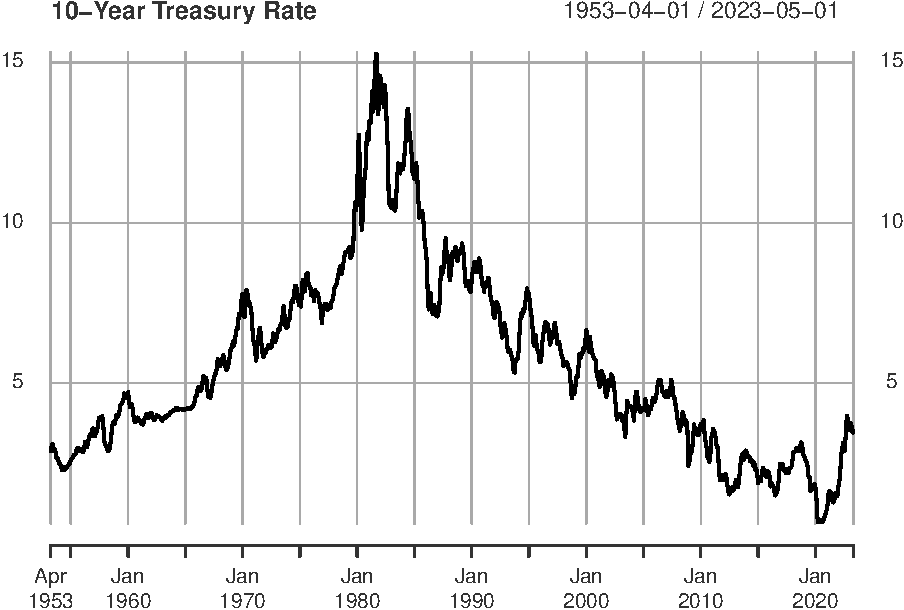
\includegraphics{_main_files/figure-latex/r-plot-1.pdf}
\caption{\label{fig:r-plot}R Plot}
\end{figure}

\begin{enumerate}
\def\labelenumi{\arabic{enumi}.}
\setcounter{enumi}{4}
\tightlist
\item
  Click on \texttt{Source}: 
\includegraphics{files/icons-rstudio/source.png} (or use the shortcut Ctrl+Shift+Enter or Cmd+Shift+Return).
\end{enumerate}

You should now see a plot of the 10-year Treasury rate on your screen. Compare it to the rate displayed on \href{https://fred.stlouisfed.org/series/GS10}{fred.stlouisfed.org/series/GS10}.

\hypertarget{save-plot-as-pdf}{%
\subsubsection*{Save Plot as PDF}\label{save-plot-as-pdf}}
\addcontentsline{toc}{subsubsection}{Save Plot as PDF}

Continue with the following steps in RStudio:

\begin{enumerate}
\def\labelenumi{\arabic{enumi}.}
\setcounter{enumi}{5}
\tightlist
\item
  Add the line: \texttt{pdf(file="myplot.pdf",width=6,height=4)} before the plot function, and add \texttt{dev.off()} after the plot:
\end{enumerate}

\begin{Shaded}
\begin{Highlighting}[]
\FunctionTok{library}\NormalTok{(}\StringTok{"quantmod"}\NormalTok{)}
\NormalTok{treasury10y }\OtherTok{\textless{}{-}} \FunctionTok{getSymbols}\NormalTok{(}\AttributeTok{Symbols =} \StringTok{"GS10"}\NormalTok{, }\AttributeTok{src =} \StringTok{"FRED"}\NormalTok{, }\AttributeTok{auto.assign =} \ConstantTok{FALSE}\NormalTok{)}
\FunctionTok{pdf}\NormalTok{(}\AttributeTok{file =} \StringTok{"myplot.pdf"}\NormalTok{, }\AttributeTok{width =} \DecValTok{6}\NormalTok{, }\AttributeTok{height =} \DecValTok{4}\NormalTok{)}
\FunctionTok{plot}\NormalTok{(treasury10y, }\AttributeTok{main =} \StringTok{"10{-}Year Treasury Rate"}\NormalTok{)}
\FunctionTok{dev.off}\NormalTok{()}
\end{Highlighting}
\end{Shaded}

\begin{enumerate}
\def\labelenumi{\arabic{enumi}.}
\setcounter{enumi}{6}
\tightlist
\item
  Click on \texttt{Source}: 
\includegraphics{files/icons-rstudio/source.png} (or use the shortcut Ctrl+Shift+Enter or Cmd+Shift+Return).
\item
  Now navigate to the same folder on your computer where you saved the R script.
\item
  There should be a file called \texttt{myplot.pdf} - open it.
\end{enumerate}

You should now see the PDF version of the plot displaying the Treasury rate. If you encounter no error message but cannot locate the \texttt{myplot.pdf} file, it's possible that R saved it in a different folder than where the R script is located. To check where R saves the plot, type \texttt{getwd()} in the console, which stands for ``get working directory.'' If you want to change the working directory and have R save the files in a different folder, type \texttt{setwd("/Users/.../...")}, replacing \texttt{"/Users/.../..."} with the path to the desired folder.

\hypertarget{run-marked-code}{%
\subsubsection*{Run Marked Code}\label{run-marked-code}}
\addcontentsline{toc}{subsubsection}{Run Marked Code}

To run only one line or one variable, mark it and then click \texttt{Run}: 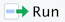
\includegraphics{files/icons-rstudio/run.png} (or use the shortcut Ctrl+Enter or Cmd+Return). Follow these steps in RStudio:

\begin{enumerate}
\def\labelenumi{\arabic{enumi}.}
\setcounter{enumi}{9}
\tightlist
\item
  Mark the variable \texttt{treasury10y}:
\end{enumerate}

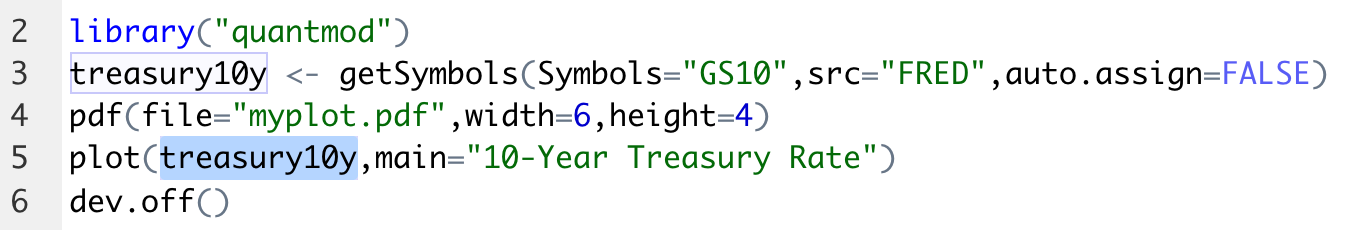
\includegraphics[width=0.7\textwidth,height=\textheight]{files/icons-rstudio/markvariable.png}

\begin{enumerate}
\def\labelenumi{\arabic{enumi}.}
\setcounter{enumi}{10}
\tightlist
\item
  Click \texttt{Run}: 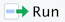
\includegraphics{files/icons-rstudio/run.png} (or use shortcut Ctrl+Enter or Cmd+Return)
\end{enumerate}

You should see the data displayed in your console, ending with 2023-05-01 3.57.

\hypertarget{create-pdf-with-r-markdown}{%
\subsubsection*{Create PDF with R Markdown}\label{create-pdf-with-r-markdown}}
\addcontentsline{toc}{subsubsection}{Create PDF with R Markdown}

Next, let's ensure that \href{https://rmarkdown.rstudio.com/}{\texttt{R\ Markdown}} is working. If you have installed \href{https://www.latex-project.org/}{\texttt{LaTeX}} and \texttt{knitr}, follow these steps in RStudio:

\begin{enumerate}
\def\labelenumi{\arabic{enumi}.}
\setcounter{enumi}{11}
\tightlist
\item
  Click on the top-left plus sign 
\includegraphics{files/icons-rstudio/plus.png} then click \texttt{R\ Markdown...}
\item
  A dialog box will appear - select \texttt{Document} and choose \texttt{PDF}, then click \texttt{OK}:
\end{enumerate}

\begin{figure}
\centering
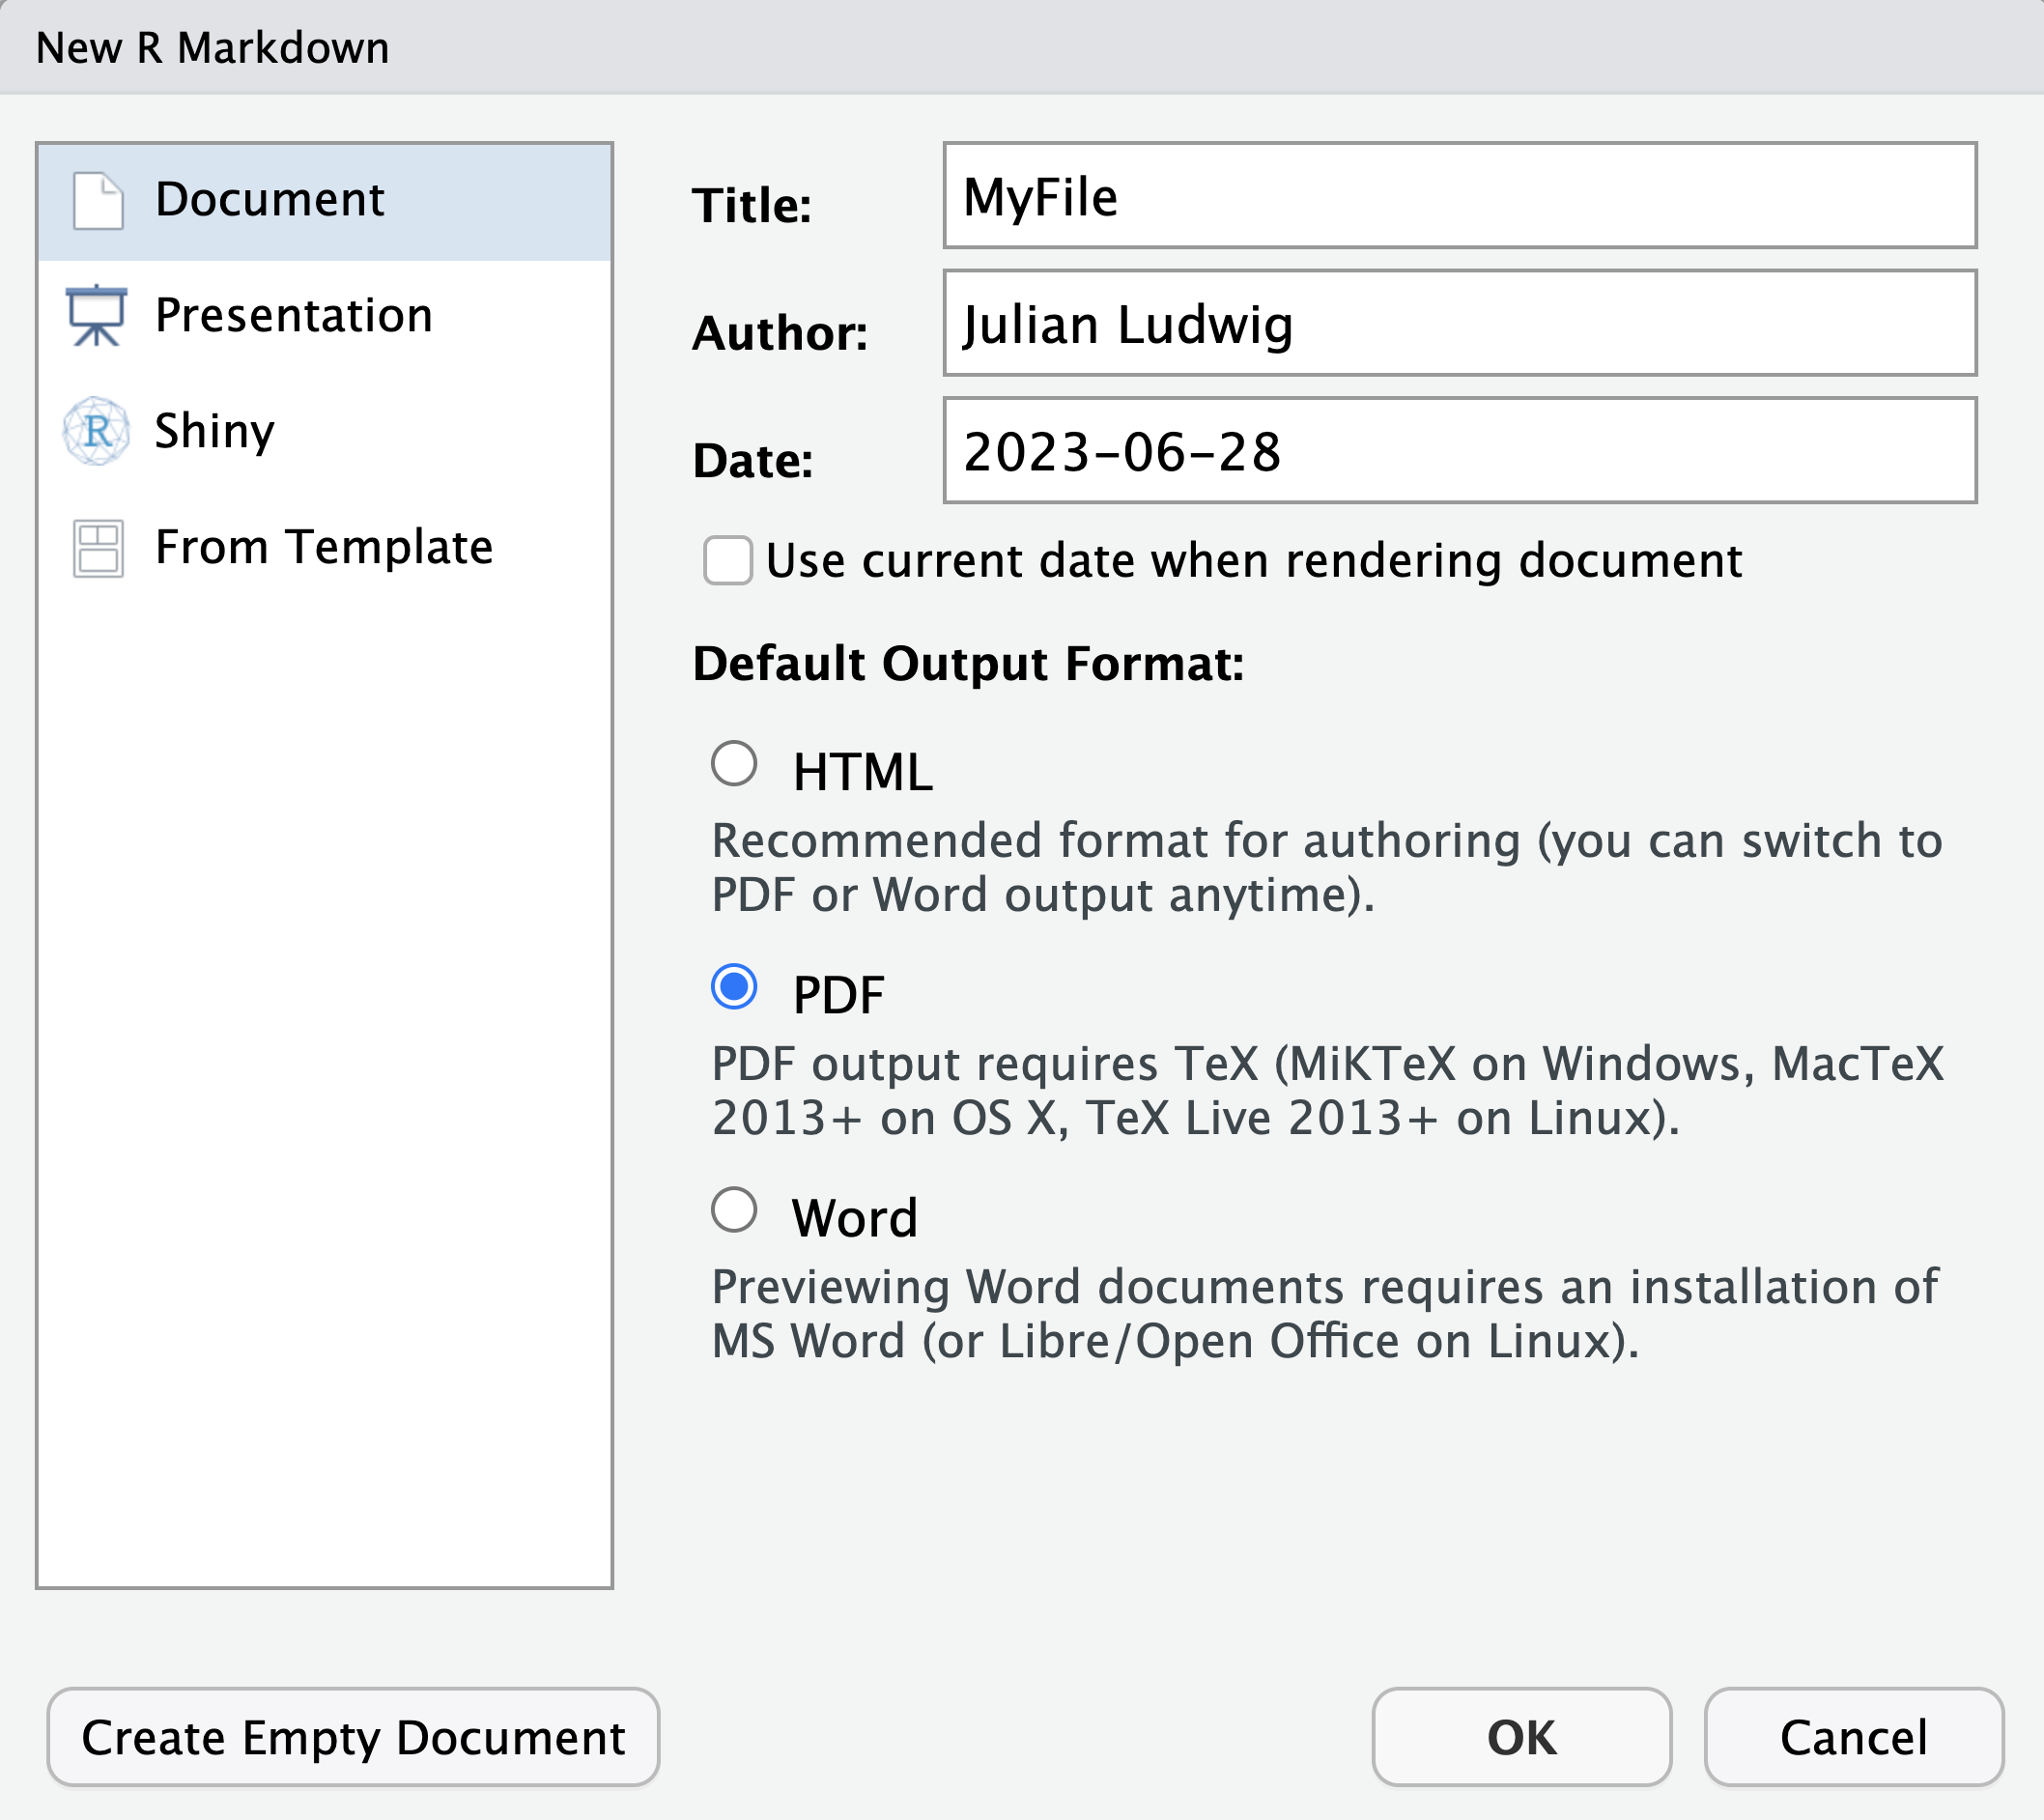
\includegraphics{files/icons-rstudio/openrmarkdown-big.png}
\caption{\label{fig:new-rmarkdown}New R Markdown}
\end{figure}

You should now see a file with text and code.

\begin{enumerate}
\def\labelenumi{\arabic{enumi}.}
\setcounter{enumi}{13}
\tightlist
\item
  Click \texttt{File} - \texttt{Save\ As...} and choose a familiar folder to save the file.
\item
  Click \texttt{Knit}: 
\includegraphics{files/icons-rstudio/knit.png} (or use the shortcut Ctrl+Shift+K or Cmd+Shift+K).
\end{enumerate}

A PDF file should appear on your screen and also in your chosen folder.

\begin{enumerate}
\def\labelenumi{\arabic{enumi}.}
\setcounter{enumi}{15}
\tightlist
\item
  Next, locate the following lines:
\end{enumerate}

\begin{Shaded}
\begin{Highlighting}[]
\DecValTok{16} \StringTok{\textasciigrave{}\textasciigrave{}\textasciigrave{}}\AttributeTok{\{r cars\}}
\AttributeTok{17 summary(cars)}
\AttributeTok{18 }\StringTok{\textasciigrave{}\textasciigrave{}\textasciigrave{}}
\end{Highlighting}
\end{Shaded}

\begin{enumerate}
\def\labelenumi{\arabic{enumi}.}
\setcounter{enumi}{16}
\tightlist
\item
  Replace these lines with the following (do not copy the line numbers):
\end{enumerate}

\begin{Shaded}
\begin{Highlighting}[]
\DecValTok{16} \StringTok{\textasciigrave{}\textasciigrave{}\textasciigrave{}}\AttributeTok{\{r, message=FALSE,warning=FALSE,echo=FALSE\}}
\AttributeTok{17 library("quantmod")}
\AttributeTok{18 treasury10y \textless{}{-} getSymbols(Symbols="GS10",src="FRED",auto.assign=FALSE)}
\AttributeTok{19 plot(treasury10y,main="10{-}Year Treasury Rate")}
\AttributeTok{20 }\StringTok{\textasciigrave{}\textasciigrave{}\textasciigrave{}}
\end{Highlighting}
\end{Shaded}

\begin{enumerate}
\def\labelenumi{\arabic{enumi}.}
\setcounter{enumi}{17}
\tightlist
\item
  Click \texttt{Knit}: 
\includegraphics{files/icons-rstudio/knit.png} (or use the shortcut Ctrl+Shift+K or Cmd+Shift+K).
\end{enumerate}

You should now see a file that looks similar to this:

\begin{figure}
\centering
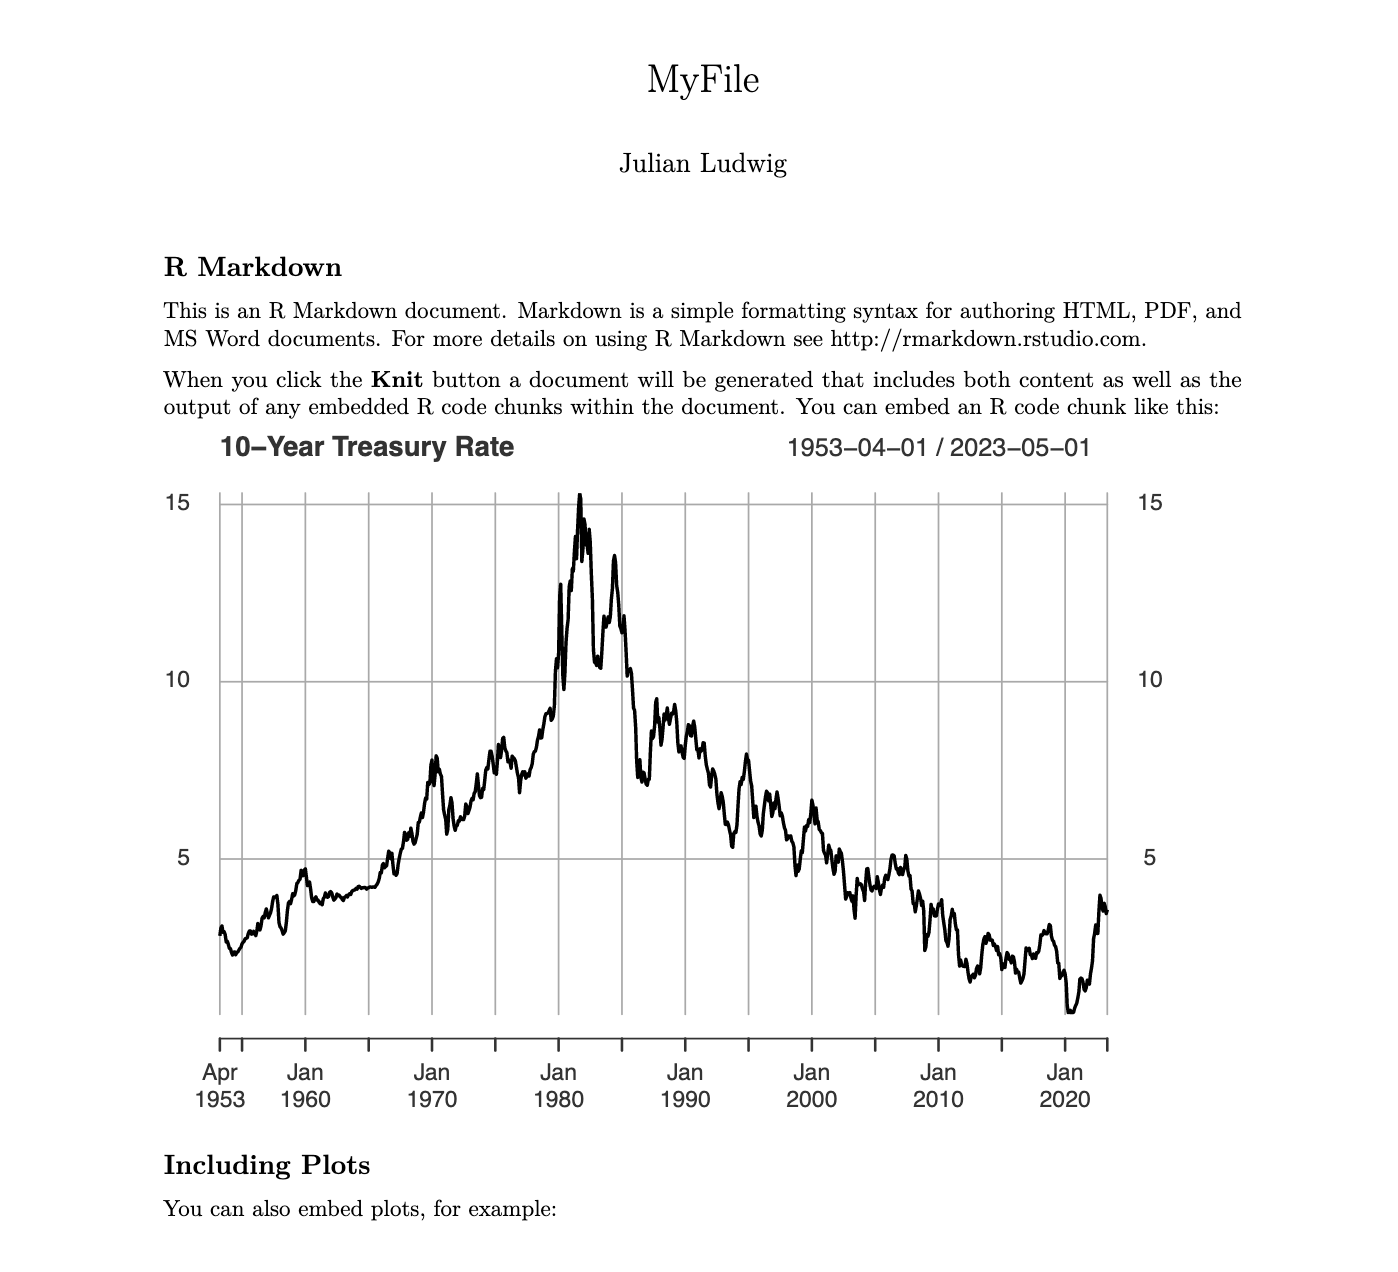
\includegraphics{files/icons-rstudio/example_rmarkdown_medium.png}
\caption{\label{fig:example-rmarkdown}PDF File Produced with R Markdown}
\end{figure}

Hint: You can set \texttt{echo=TRUE} to include R code in your report.

You can now change the title of the file and the text to create a professional report. If you click the arrow next to \texttt{Knit}: 
\includegraphics{files/icons-rstudio/knitdown.png} you have options to export your file as an HTML or Word document instead of a PDF document, which is convenient when designing a website or writing an app:

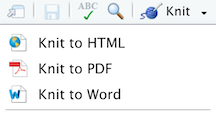
\includegraphics[width=\textwidth,height=0.85\textheight]{files/icons-rstudio/knitdownoptions.png}

\hypertarget{troubleshooting}{%
\subsubsection*{Troubleshooting}\label{troubleshooting}}
\addcontentsline{toc}{subsubsection}{Troubleshooting}

That's it! If everything worked as expected, you're good to go. If not, continue troubleshooting until it works.

\hypertarget{getting-started}{%
\chapter{Getting Started}\label{getting-started}}

R is a programming language and free software environment for statistical computing and graphics supported by the R Foundation for Statistical Computing.

\hypertarget{rstudio-interface}{%
\section{RStudio Interface}\label{rstudio-interface}}

After launching RStudio on your computer, navigate to the menu bar and select ``File,'' then choose ``New File,'' and finally click on ``R Script.'' Alternatively, you can use the keyboard shortcut Ctrl+Shift+N (Windows/Linux) or Cmd+Shift+N (Mac) to create a new R script directly.

\begin{figure}
\centering
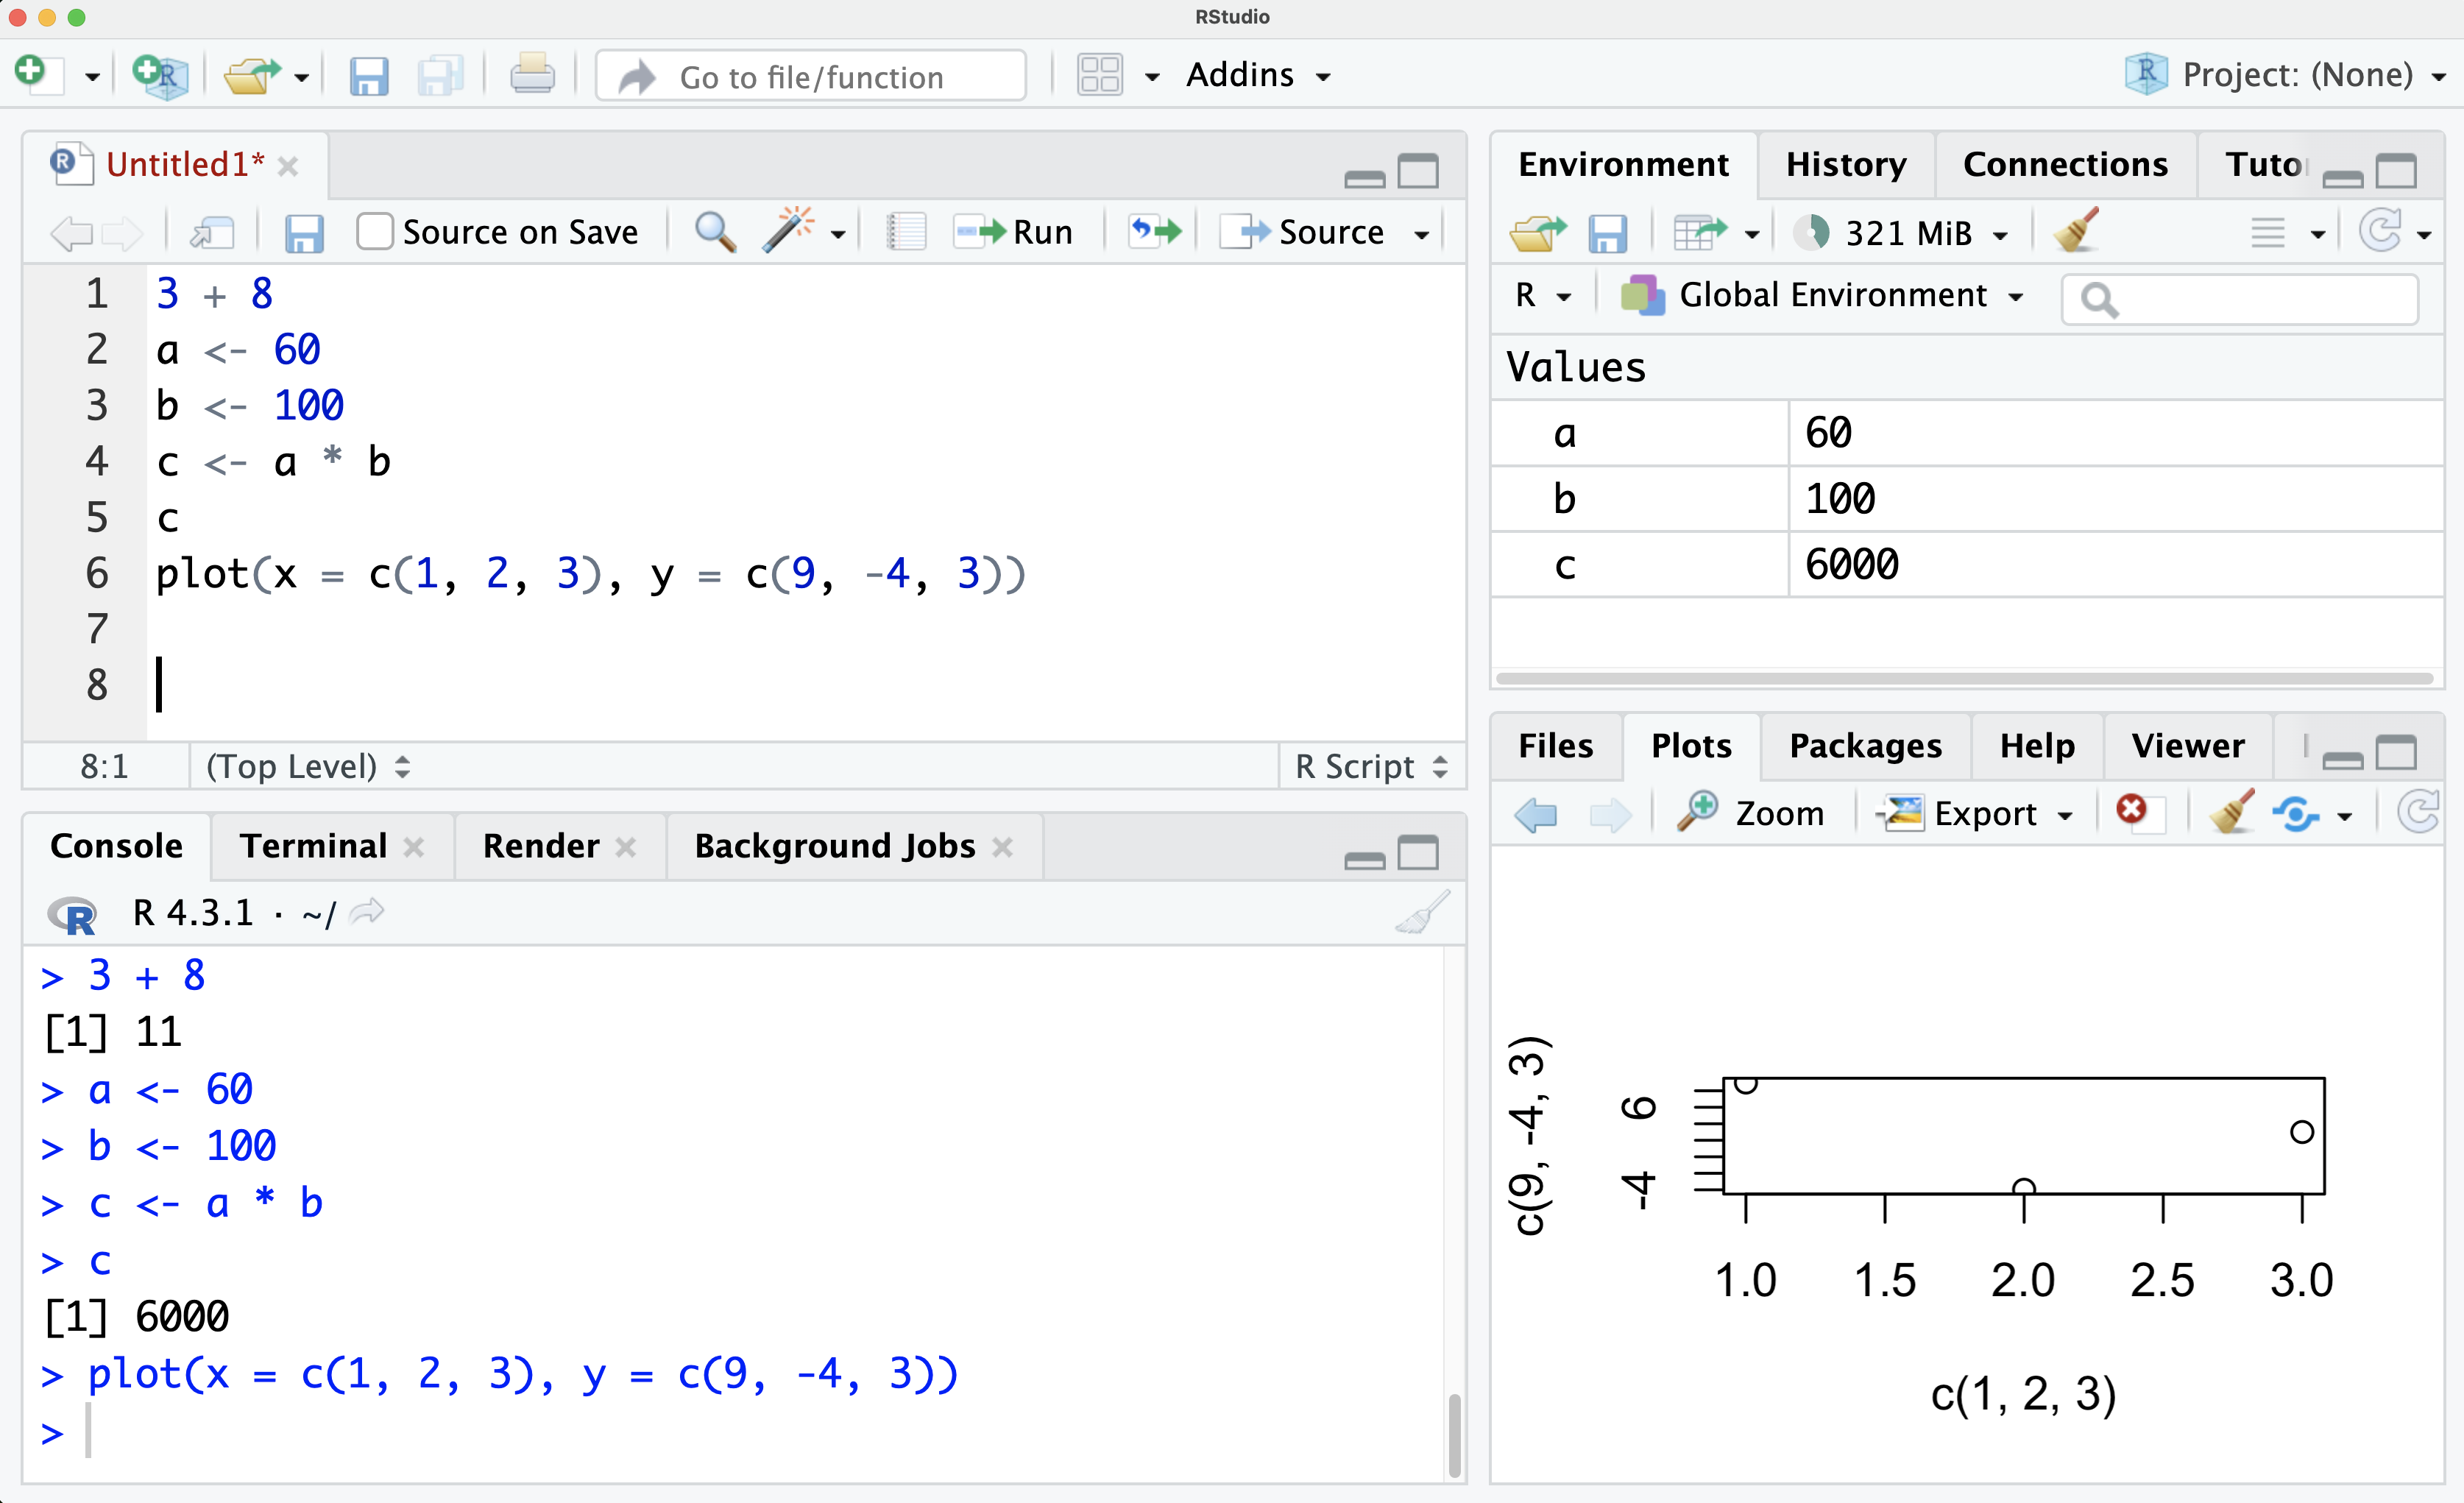
\includegraphics{files/icons-rstudio/rstudio-rscript-code.png}
\caption{\label{fig:rstudio-rscript-code}RStudio Interface}
\end{figure}

Once you have opened a new R script, you will notice that RStudio consists of four main sections:

\begin{enumerate}
\def\labelenumi{\arabic{enumi}.}
\item
  \textbf{Source} (top-left): This section is where you write your R scripts. Also known as \textbf{do-files}, R scripts are files that contain a sequence of commands which can be executed either wholly or partially. To run a single line in your script, click on that line with your cursor and press the 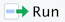
\includegraphics{files/icons-rstudio/run.png} button. However, to streamline your workflow, I recommend using the keyboard shortcut Ctrl+Enter (Windows/Linux) or Cmd+Enter (Mac) to run the line without reaching for the mouse. If you want to execute only a specific portion of a line, select that part and then press Ctrl+Enter or Cmd+Enter. To run all the commands in your R script, use the 
\includegraphics{files/icons-rstudio/source.png} button or the keyboard shortcut Ctrl+Shift+Enter (Windows/Linux) or Cmd+Shift+Enter (Mac).
\item
  \textbf{Console} (bottom-left): Located below the Source section, the Console is where R executes your commands. You can also directly type commands into the Console and see their output immediately. However, it is advisable to write commands in the R Script instead of the Console. By doing so, you can save the commands for future reference, enabling you to reproduce your results at a later time.
\item
  \textbf{Environment} (top-right): In the upper-right section, the Environment tab displays the current objects stored in memory, providing an overview of your variables, functions, and data frames. To create a variable, you can use the assignment operator \texttt{\textless{}-} (reversed arrow). Once a variable is created and assigned a numeric value, it can be utilized in arithmetic operations. For example:
\end{enumerate}

\begin{Shaded}
\begin{Highlighting}[]
\NormalTok{a }\OtherTok{\textless{}{-}} \DecValTok{60}
\NormalTok{a }\SpecialCharTok{+} \DecValTok{20}
\end{Highlighting}
\end{Shaded}

\begin{verbatim}
## [1] 80
\end{verbatim}

\begin{enumerate}
\def\labelenumi{\arabic{enumi}.}
\setcounter{enumi}{3}
\tightlist
\item
  \textbf{Files/Plots/Packages/Help/Viewer} (bottom-right): The bottom-right panel contains multiple tabs:

  \begin{itemize}
  \tightlist
  \item
    Files: displays your files and folders
  \item
    Plots: displays your graphs
  \item
    Packages: lets you manage your R packages
  \item
    Help: provides help documentation
  \item
    Viewer: lets you view local web content
  \end{itemize}
\end{enumerate}

These four main sections of RStudio provide a comprehensive environment for writing, executing, and managing your R code efficiently.

\hypertarget{r-scripts}{%
\subsubsection*{R Scripts}\label{r-scripts}}
\addcontentsline{toc}{subsubsection}{R Scripts}

An R script is a text file that contains your R code. You can execute parts of the script by selecting a subset of commands and pressing Ctrl+Enter or Cmd+Enter, or run the entire script by pressing Ctrl+Shift+Enter.

Any text written after a hashtag (\texttt{\#}) in an R Script is considered comments and is not executed as code. Comments are valuable for providing explanations or annotations for your commands, enhancing the readability and comprehensibility of your code.

\begin{Shaded}
\begin{Highlighting}[]
\CommentTok{\# This is a comment in an R script}
\NormalTok{x }\OtherTok{\textless{}{-}} \DecValTok{10}  \CommentTok{\# Assign the value 10 to x}
\NormalTok{y }\OtherTok{\textless{}{-}} \DecValTok{20}  \CommentTok{\# Assign the value 20 to y}
\NormalTok{z }\OtherTok{\textless{}{-}}\NormalTok{ x }\SpecialCharTok{+}\NormalTok{ y  }\CommentTok{\# Add x and y and assign the result to z}
\FunctionTok{print}\NormalTok{(z)  }\CommentTok{\# Print the value of z}
\end{Highlighting}
\end{Shaded}

\begin{verbatim}
## [1] 30
\end{verbatim}

The output displayed after two hashtags (\texttt{\#\#}) in the example above: \texttt{\#\#\ {[}1{]}\ 30}, is not part of the actual R Script. Instead, it represents a line you would observe in your console when running the R Script. It showcases the result or value of the variable \texttt{z} in this case.

To facilitate working with lengthy R scripts, it is recommended to use a separate window. You can open a separate window by selecting 
\includegraphics{files/icons-rstudio/show-in-new-window.png} in the top-left corner.

\begin{figure}
\centering
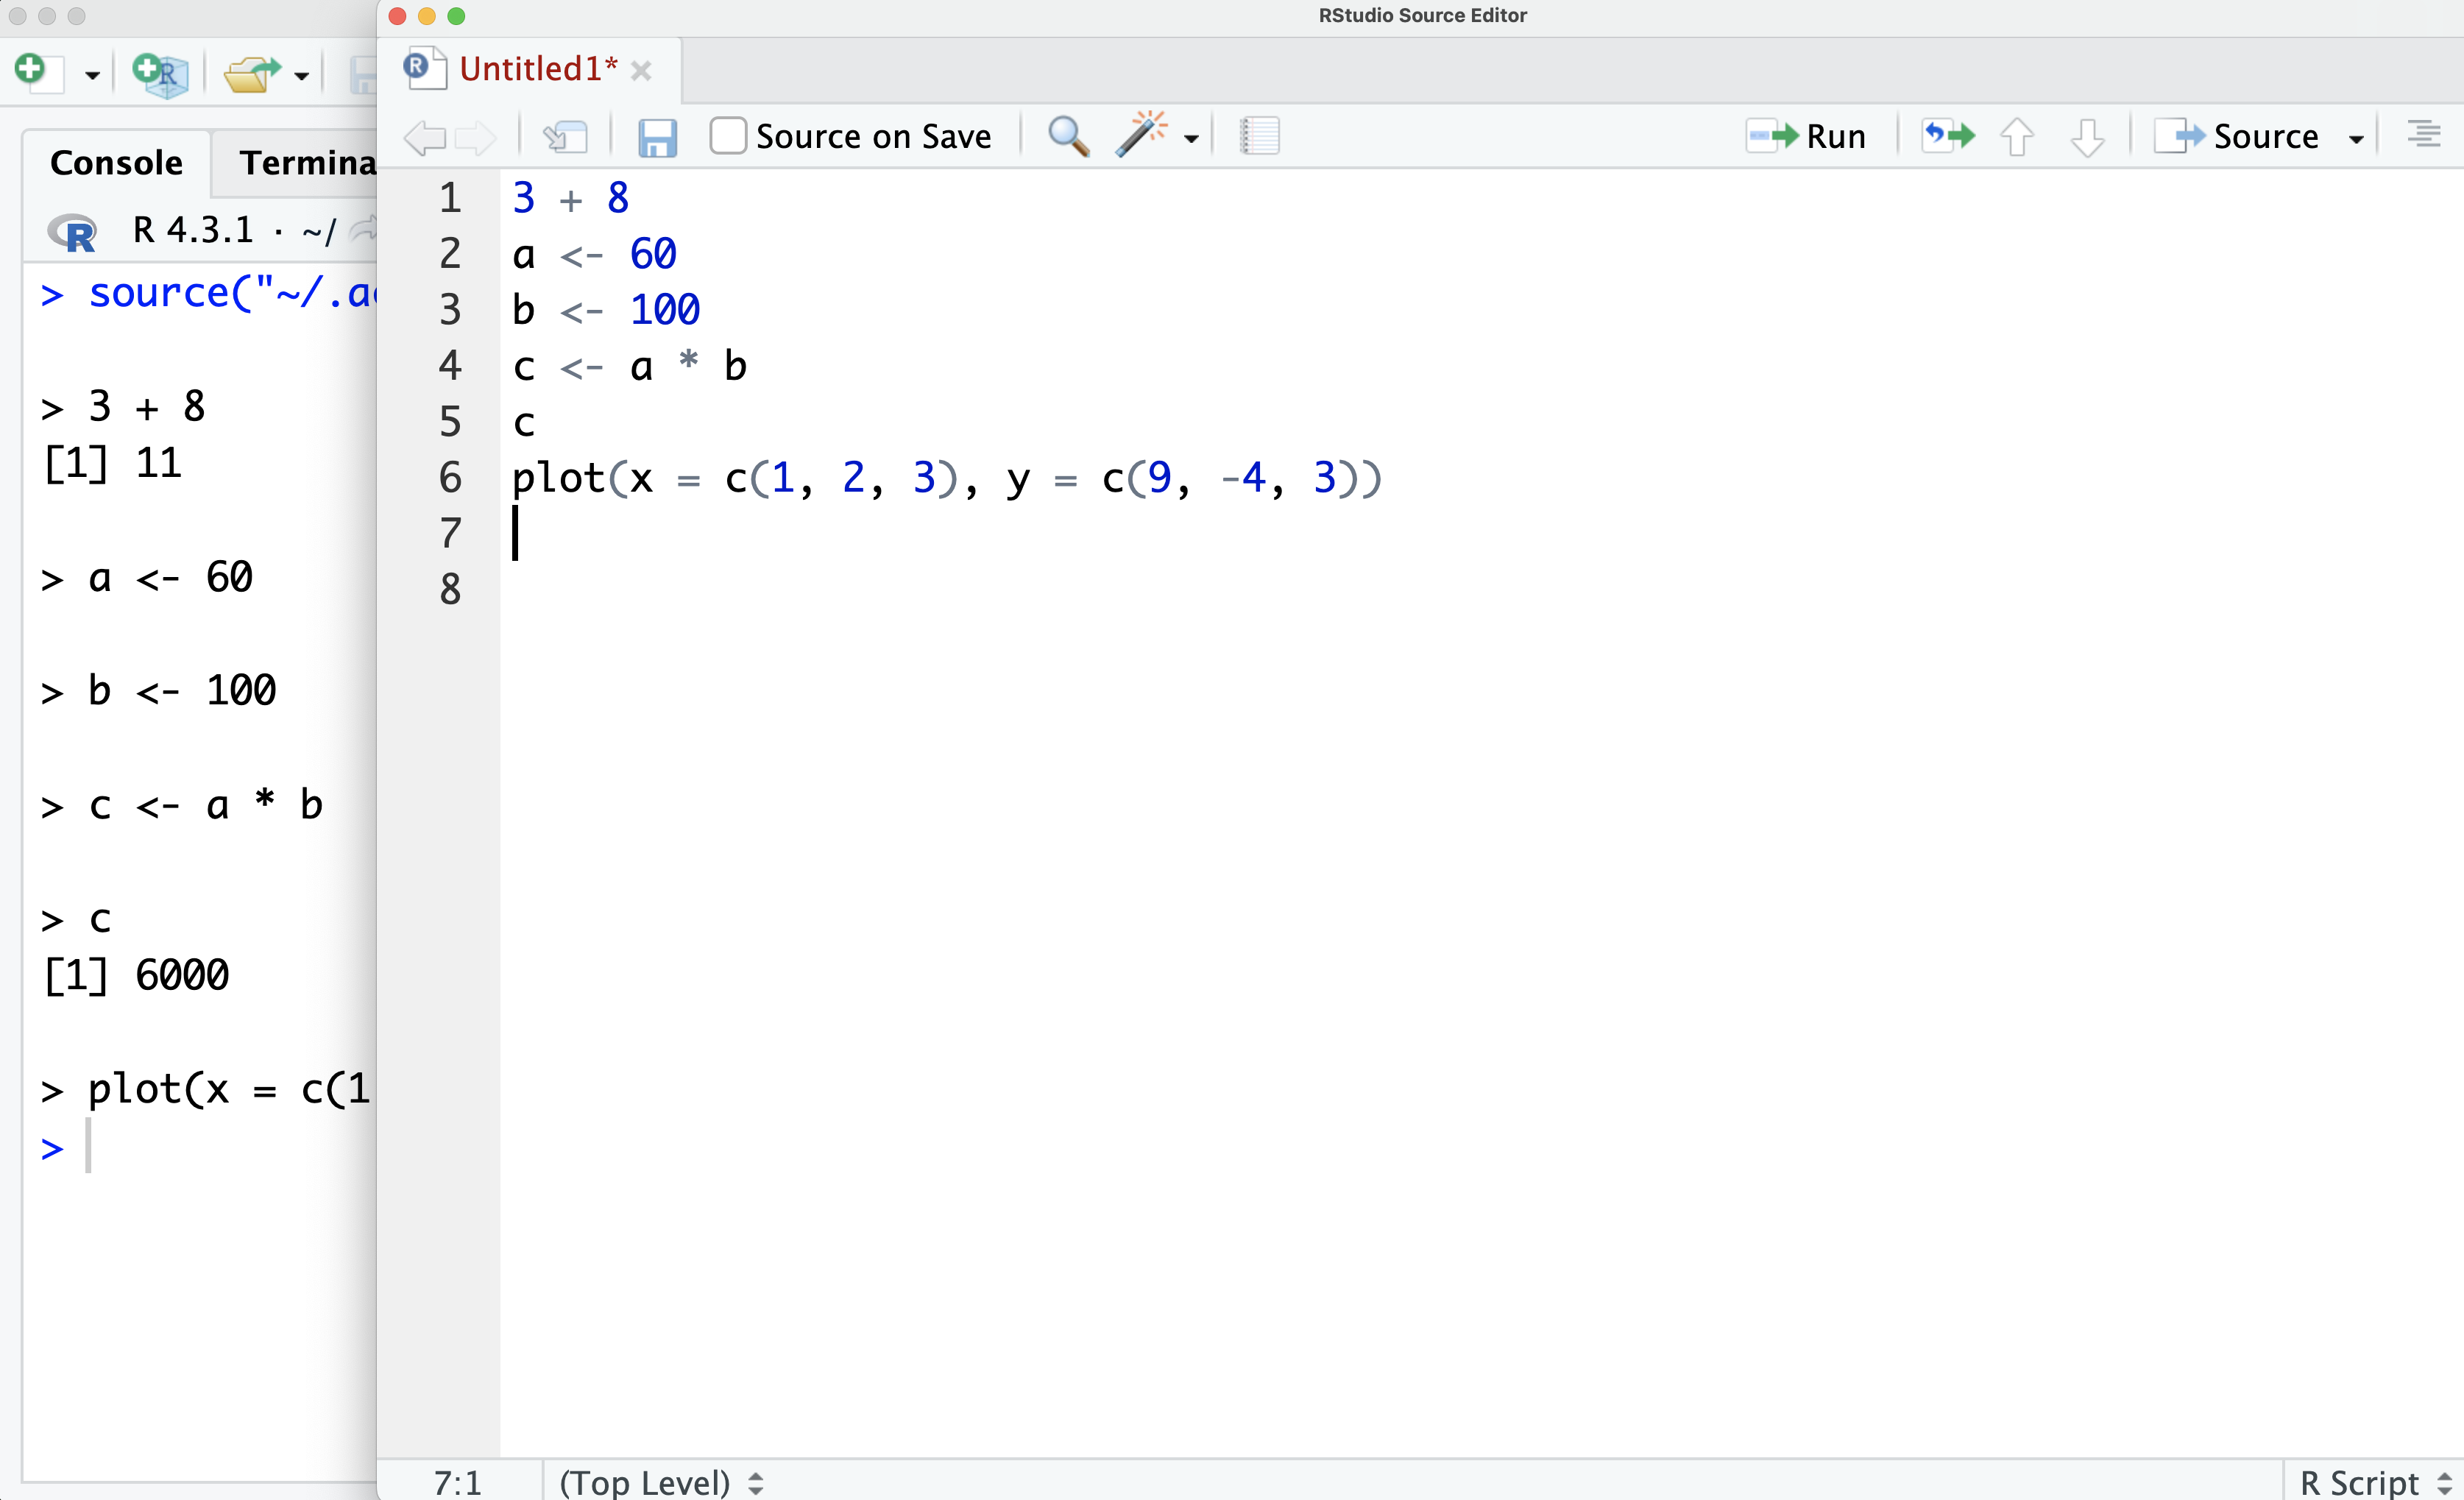
\includegraphics{files/icons-rstudio/rstudio-rscript-separate.png}
\caption{\label{fig:rstudio-rscript-separate}RStudio Interface with Separate R Script Window}
\end{figure}

When the R Script is in a separate window, you can easily switch between the R Script window and the Console/Environment/Plot Window by pressing Ctrl+Tab or Cmd+Tab. This allows for convenient navigation between different RStudio windows.

\hypertarget{r-data-types-and-structures}{%
\section{R Data Types and Structures}\label{r-data-types-and-structures}}

The R language supports a broad array of operations such as mathematical calculations, logical analyses, and text manipulation. However, the applicability of a function to a variable depends on the variable's data type. For instance, an arithmetic function to add two variables won't work if the variables store text.

R supports various data types, including numeric (\texttt{x\ \textless{}-\ 15}), character (\texttt{x\ \textless{}-\ "Hello!"}), and logical (\texttt{x\ \textless{}-\ TRUE} or \texttt{x\ \textless{}-\ FALSE}). In addition to single values (scalars), R allows variables to hold collections of numbers or strings using vectors, matrices, lists, or data frames. Advanced data structures such as tibbles, data tables, and \texttt{xts} objects provide additional features beyond traditional data frames.

In this section, we will explore the following data types:

\begin{enumerate}
\def\labelenumi{\arabic{enumi}.}
\tightlist
\item
  \textbf{Scalar}: A single data element, such as a number or a character string.
\item
  \textbf{Vector}: A one-dimensional array that contains elements of the same type.
\item
  \textbf{Matrix} (\texttt{matrix}): A two-dimensional array with elements of the same type.
\item
  \textbf{List} (\texttt{list}): A one-dimensional array capable of storing various data types.
\item
  \textbf{Data Frame} (\texttt{data.frame}): A two-dimensional array that can accommodate columns of different types.
\item
  \textbf{Tibble} (\texttt{tibble}): An enhanced version of data frames, offering user-friendly features.
\item
  \textbf{Data Table} (\texttt{data.table}): An optimized data frame extension designed for speed and handling large datasets.
\item
  \textbf{Extensible Time Series} (\texttt{xts}): A time-indexed data frame specifically designed for time series data.
\end{enumerate}

Understanding the data type of variables is crucial because it determines the operations and functions that can be applied to them.

It's worth noting that R provides so-called \textbf{wrapper functions}, which are functions that have the same name but perform different actions depending on the data object. These wrapper functions adapt their behavior based on the input data type, allowing for more flexible and intuitive programming. For example, the \texttt{summary()} function in R is a wrapper function. When applied to a numeric vector, it provides statistical summaries such as mean, median, and quartiles. However, when applied to a data frame, it gives a summary of each variable, including the minimum, maximum, and quartiles for numerical variables, as well as counts and levels for categorical variables.

\hypertarget{scalar}{%
\subsection{Scalar}\label{scalar}}

Scalars in R are variables holding single objects. You can determine an object's type by applying the \texttt{class()} function to the variable.

\hypertarget{numbers-characters-and-logical-values}{%
\subsubsection*{Numbers, Characters, and Logical Values}\label{numbers-characters-and-logical-values}}
\addcontentsline{toc}{subsubsection}{Numbers, Characters, and Logical Values}

\begin{Shaded}
\begin{Highlighting}[]
\CommentTok{\# Numeric (a.k.a. Double)}
\NormalTok{w }\OtherTok{\textless{}{-}} \FloatTok{5.5}  \CommentTok{\# w is a decimal number.}
\FunctionTok{class}\NormalTok{(w)  }\CommentTok{\# Returns "numeric".}

\CommentTok{\# Integer}
\NormalTok{x }\OtherTok{\textless{}{-}}\NormalTok{ 10L  }\CommentTok{\# The L tells R to store x as an integer instead of a decimal number.}
\FunctionTok{class}\NormalTok{(x)  }\CommentTok{\# Returns "integer".}

\CommentTok{\# Complex}
\NormalTok{u }\OtherTok{\textless{}{-}} \DecValTok{3} \SpecialCharTok{+}\NormalTok{ 4i }\CommentTok{\# u is a complex number, where 3 is real and 4 is imaginary.}
\FunctionTok{class}\NormalTok{(u)  }\CommentTok{\# Returns "complex".}

\CommentTok{\# Character}
\NormalTok{y }\OtherTok{\textless{}{-}} \StringTok{"Hello, World!"}  \CommentTok{\# y is a character string.}
\FunctionTok{class}\NormalTok{(y)  }\CommentTok{\# Returns "character".}

\CommentTok{\# Logical}
\NormalTok{z }\OtherTok{\textless{}{-}} \ConstantTok{TRUE}  \CommentTok{\# z is a logical value.}
\FunctionTok{class}\NormalTok{(z)  }\CommentTok{\# Returns "logical".}
\end{Highlighting}
\end{Shaded}

\begin{verbatim}
## [1] "numeric"
## [1] "integer"
## [1] "complex"
## [1] "character"
## [1] "logical"
\end{verbatim}

An object's type dictates which functions can be applied. For example, mathematical functions are applicable to numbers but not characters:

\begin{Shaded}
\begin{Highlighting}[]
\CommentTok{\# Mathematical operations}
\DecValTok{2} \SpecialCharTok{+} \DecValTok{2}  \CommentTok{\# Results in 4.}
\DecValTok{3} \SpecialCharTok{*} \DecValTok{5}  \CommentTok{\# Results in 15.}
\NormalTok{(}\DecValTok{1} \SpecialCharTok{+} \DecValTok{2}\NormalTok{) }\SpecialCharTok{*} \DecValTok{3}  \CommentTok{\# Results in 9 (parentheses take precedence).}

\CommentTok{\# Logical operations}
\ConstantTok{TRUE} \SpecialCharTok{\&} \ConstantTok{FALSE}  \CommentTok{\# Results in FALSE (logical AND).}
\ConstantTok{TRUE} \SpecialCharTok{|} \ConstantTok{FALSE}  \CommentTok{\# Results in TRUE (logical OR).}

\CommentTok{\# String operations}
\FunctionTok{paste}\NormalTok{(}\StringTok{"Hello"}\NormalTok{, }\StringTok{"World!"}\NormalTok{)  }\CommentTok{\# Concatenates strings, results in "Hello World!".}
\FunctionTok{nchar}\NormalTok{(}\StringTok{"Hello"}\NormalTok{)  }\CommentTok{\# Counts characters in a string, results in 5.}
\end{Highlighting}
\end{Shaded}

\begin{verbatim}
## [1] 4
## [1] 15
## [1] 9
## [1] FALSE
## [1] TRUE
## [1] "Hello World!"
## [1] 5
\end{verbatim}

\hypertarget{dates-and-times}{%
\subsubsection*{Dates and Times}\label{dates-and-times}}
\addcontentsline{toc}{subsubsection}{Dates and Times}

In this course, we also deal with data types specifically designed for storing date and time information:

\begin{Shaded}
\begin{Highlighting}[]
\CommentTok{\# Date}
\NormalTok{v }\OtherTok{\textless{}{-}} \FunctionTok{as.Date}\NormalTok{(}\StringTok{"2023{-}06{-}30"}\NormalTok{)  }\CommentTok{\# v is a Date.}
\CommentTok{\# The default input format is \%Y{-}\%m{-}\%d, where}
\CommentTok{\# {-} \%Y is year in 4 digits,}
\CommentTok{\# {-} \%m is month with 2 digits, and }
\CommentTok{\# {-} \%d is day with 2 digits.}
\FunctionTok{class}\NormalTok{(v)  }\CommentTok{\# Returns "Date".}
\end{Highlighting}
\end{Shaded}

\begin{verbatim}
## [1] "Date"
\end{verbatim}

\begin{Shaded}
\begin{Highlighting}[]
\CommentTok{\# POSIXct (Time)}
\NormalTok{t }\OtherTok{\textless{}{-}} \FunctionTok{as.POSIXct}\NormalTok{(}\StringTok{"2023{-}06{-}30 18:47:10"}\NormalTok{, }\AttributeTok{tz =} \StringTok{"CDT"}\NormalTok{)  }\CommentTok{\# t is a POSIXct.}
\end{Highlighting}
\end{Shaded}

\begin{verbatim}
## Warning in strptime(xx, f, tz = tz): unknown timezone 'CDT'
\end{verbatim}

\begin{verbatim}
## Warning in as.POSIXct.POSIXlt(x): unknown timezone 'CDT'
\end{verbatim}

\begin{verbatim}
## Warning in strptime(x, f, tz = tz): unknown timezone 'CDT'
\end{verbatim}

\begin{verbatim}
## Warning in as.POSIXct.POSIXlt(as.POSIXlt(x, tz, ...), tz, ...): unknown
## timezone 'CDT'
\end{verbatim}

\begin{Shaded}
\begin{Highlighting}[]
\CommentTok{\# The default input format is \%Y{-}\%m{-}\%d \%H:\%M:\%S, where}
\CommentTok{\# {-} \%H is hour out of 24,}
\CommentTok{\# {-} \%M is minute out of 60, and}
\CommentTok{\# {-} \%S is second out of 60.}
\CommentTok{\# The tz input is the time zone, where CDT = Central Daylight Time.}
\FunctionTok{class}\NormalTok{(t)  }\CommentTok{\# Returns "POSIXct".}
\end{Highlighting}
\end{Shaded}

\begin{verbatim}
## [1] "POSIXct" "POSIXt"
\end{verbatim}

The default input format, \texttt{\%Y-\%m-\%d} or \texttt{\%Y-\%m-\%d\ \%H:\%M:\%S}, can be changed by specifying a format input. The output format can be adjusted by applying the \texttt{format()} function to the object:

\begin{Shaded}
\begin{Highlighting}[]
\CommentTok{\# Date with custom input format:}
\NormalTok{v }\OtherTok{\textless{}{-}} \FunctionTok{as.Date}\NormalTok{(}\StringTok{"April 6 {-}{-} 23"}\NormalTok{, }\AttributeTok{format =} \StringTok{"\%B \%d {-}{-} \%y"}\NormalTok{)}
\NormalTok{v  }\CommentTok{\# Returns default output format: \%Y{-}\%m{-}\%d.}
\end{Highlighting}
\end{Shaded}

\begin{verbatim}
## [1] "2023-04-06"
\end{verbatim}

\begin{Shaded}
\begin{Highlighting}[]
\FunctionTok{format}\NormalTok{(v, }\AttributeTok{format =} \StringTok{"\%B \%d, \%Y"}\NormalTok{)  }\CommentTok{\# Returns a custom output format: "\%B \%d, \%Y".}
\end{Highlighting}
\end{Shaded}

\begin{verbatim}
## [1] "April 06, 2023"
\end{verbatim}

The syntax for different date formats can be found by typing \texttt{?strptime} in the R console. Some of the most commonly used formats are outlined in the table below:

\begin{tabular}{l|l|l}
\hline
Specification & Description & Example\\
\hline
\%a & Abbreviated weekday & Sun, Thu\\
\hline
\%A & Full weekday & Sunday, Thursday\\
\hline
\%b or \%h & Abbreviated month & May, Jul\\
\hline
\%B & Full month & May, July\\
\hline
\%d & Day of the month, 0-31 & 27, 07\\
\hline
\%j & Day of the year, 001-366 & 148, 188\\
\hline
\%m & Month, 01-12 & 05, 07\\
\hline
\%U & Week, 01-53, with Sunday as first day of the week & 22, 27\\
\hline
\%w & Weekday, 0-6, Sunday is 0 & 0, 4\\
\hline
\%W & Week, 00-53, with Monday as first day of the week & 21, 27\\
\hline
\%x & Date, locale-specific & \\
\hline
\%y & Year without century, 00-99 & 84, 05\\
\hline
\%Y & Year with century, on input: 00 to 68 prefixed by 20, 69 to 99 prefixed by 19 & 1984, 2005\\
\hline
\%C & Century & 19, 20\\
\hline
\%D & Date formatted \%m/\%d/\%y & 5/27/84\\
\hline
\%u & Weekday, 1-7, Monday is 1 & 7, 4\\
\hline
\%n & Newline on output or arbitrary whitespace on input & \\
\hline
\%t & Tab on output or arbitrary whitespace on input & \\
\hline
\end{tabular}

Here are some example operations for \texttt{Date} objects:

\begin{Shaded}
\begin{Highlighting}[]
\CommentTok{\# Date Operations}
\NormalTok{date1 }\OtherTok{\textless{}{-}} \FunctionTok{as.Date}\NormalTok{(}\StringTok{"2023{-}06{-}30"}\NormalTok{)}
\NormalTok{date2 }\OtherTok{\textless{}{-}} \FunctionTok{as.Date}\NormalTok{(}\StringTok{"2023{-}01{-}01"}\NormalTok{)}

\CommentTok{\# Subtract dates to get the number of days between}
\NormalTok{days\_between }\OtherTok{\textless{}{-}}\NormalTok{ date1 }\SpecialCharTok{{-}}\NormalTok{ date2}
\NormalTok{days\_between}
\end{Highlighting}
\end{Shaded}

\begin{verbatim}
## Time difference of 180 days
\end{verbatim}

\begin{Shaded}
\begin{Highlighting}[]
\CommentTok{\# Add days to a date}
\NormalTok{date\_in\_future }\OtherTok{\textless{}{-}}\NormalTok{ date1 }\SpecialCharTok{+} \DecValTok{30}
\NormalTok{date\_in\_future}
\end{Highlighting}
\end{Shaded}

\begin{verbatim}
## [1] "2023-07-30"
\end{verbatim}

\hypertarget{vector}{%
\subsection{Vector}\label{vector}}

In R, a vector is a homogeneous sequence of elements, meaning they must all be of the same basic type. As such, a vector can hold multiple numbers, but it cannot mix types, such as having both numbers and words. The function \texttt{c()} (for combine) can be used to create a vector:

\begin{Shaded}
\begin{Highlighting}[]
\CommentTok{\# Numeric vector}
\NormalTok{numeric\_vector }\OtherTok{\textless{}{-}} \FunctionTok{c}\NormalTok{(}\DecValTok{1}\NormalTok{, }\DecValTok{2}\NormalTok{, }\DecValTok{3}\NormalTok{, }\DecValTok{4}\NormalTok{, }\DecValTok{5}\NormalTok{)}
\FunctionTok{class}\NormalTok{(numeric\_vector)  }\CommentTok{\# Returns "numeric".}

\CommentTok{\# Character vector}
\NormalTok{character\_vector }\OtherTok{\textless{}{-}} \FunctionTok{c}\NormalTok{(}\StringTok{"Hello"}\NormalTok{, }\StringTok{"World"}\NormalTok{, }\StringTok{"!"}\NormalTok{)}
\FunctionTok{class}\NormalTok{(character\_vector)  }\CommentTok{\# Returns "character".}

\CommentTok{\# Logical vector}
\NormalTok{logical\_vector }\OtherTok{\textless{}{-}} \FunctionTok{c}\NormalTok{(}\ConstantTok{TRUE}\NormalTok{, }\ConstantTok{FALSE}\NormalTok{, }\ConstantTok{TRUE}\NormalTok{)}
\FunctionTok{class}\NormalTok{(logical\_vector)  }\CommentTok{\# Returns "logical".}
\end{Highlighting}
\end{Shaded}

\begin{verbatim}
## [1] "numeric"
## [1] "character"
## [1] "logical"
\end{verbatim}

The function \texttt{c()} can also be used to add elements to a vector:

\begin{Shaded}
\begin{Highlighting}[]
\CommentTok{\# Add elements to existing vector:}
\NormalTok{x }\OtherTok{\textless{}{-}} \FunctionTok{c}\NormalTok{(}\DecValTok{1}\NormalTok{, }\DecValTok{2}\NormalTok{, }\DecValTok{3}\NormalTok{)}
\NormalTok{x }\OtherTok{\textless{}{-}} \FunctionTok{c}\NormalTok{(x, }\DecValTok{4}\NormalTok{, }\DecValTok{5}\NormalTok{, }\DecValTok{6}\NormalTok{)}
\NormalTok{x}
\end{Highlighting}
\end{Shaded}

\begin{verbatim}
## [1] 1 2 3 4 5 6
\end{verbatim}

The \texttt{sec()} function creates a sequence of numbers or dates:

\begin{Shaded}
\begin{Highlighting}[]
\CommentTok{\# Create a sequence of numbers:}
\NormalTok{x }\OtherTok{\textless{}{-}} \FunctionTok{seq}\NormalTok{(}\AttributeTok{from =} \DecValTok{1}\NormalTok{, }\AttributeTok{to =} \FloatTok{1.5}\NormalTok{, }\AttributeTok{by =} \FloatTok{0.1}\NormalTok{)}
\NormalTok{x}
\end{Highlighting}
\end{Shaded}

\begin{verbatim}
## [1] 1.0 1.1 1.2 1.3 1.4 1.5
\end{verbatim}

\begin{Shaded}
\begin{Highlighting}[]
\CommentTok{\# Create a sequence of dates:}
\NormalTok{x }\OtherTok{\textless{}{-}} \FunctionTok{seq}\NormalTok{(}\AttributeTok{from =} \FunctionTok{as.Date}\NormalTok{(}\StringTok{"2004{-}05{-}01"}\NormalTok{), }\AttributeTok{to =} \FunctionTok{as.Date}\NormalTok{(}\StringTok{"2004{-}12{-}01"}\NormalTok{), }\AttributeTok{by =} \StringTok{"month"}\NormalTok{)}
\NormalTok{x}
\end{Highlighting}
\end{Shaded}

\begin{verbatim}
## [1] "2004-05-01" "2004-06-01" "2004-07-01" "2004-08-01" "2004-09-01"
## [6] "2004-10-01" "2004-11-01" "2004-12-01"
\end{verbatim}

Missing data is represented as \texttt{NA} (not available). The function \texttt{is.na()} indicates the elements that are missing and \texttt{anyNA()} returns TRUE if the vector contains any missing values:

\begin{Shaded}
\begin{Highlighting}[]
\NormalTok{x }\OtherTok{\textless{}{-}} \FunctionTok{c}\NormalTok{(}\DecValTok{1}\NormalTok{, }\DecValTok{2}\NormalTok{, }\ConstantTok{NA}\NormalTok{, }\ConstantTok{NA}\NormalTok{, }\DecValTok{4}\NormalTok{, }\DecValTok{9}\NormalTok{, }\DecValTok{12}\NormalTok{, }\DecValTok{5}\NormalTok{, }\DecValTok{4}\NormalTok{, }\ConstantTok{NA}\NormalTok{)}
\FunctionTok{is.na}\NormalTok{(x)}
\end{Highlighting}
\end{Shaded}

\begin{verbatim}
##  [1] FALSE FALSE  TRUE  TRUE FALSE FALSE FALSE FALSE FALSE  TRUE
\end{verbatim}

\begin{Shaded}
\begin{Highlighting}[]
\FunctionTok{anyNA}\NormalTok{(x)}
\end{Highlighting}
\end{Shaded}

\begin{verbatim}
## [1] TRUE
\end{verbatim}

A generalization of logical vectors are \textbf{factors}, which are vectors that restrict entries to be one of predefined categories:

\begin{Shaded}
\begin{Highlighting}[]
\CommentTok{\# Unordered factors, e.g. categories "Male" and "Female":}
\NormalTok{gender\_vector }\OtherTok{\textless{}{-}} \FunctionTok{c}\NormalTok{(}\StringTok{"Male"}\NormalTok{, }\StringTok{"Female"}\NormalTok{, }\StringTok{"Male"}\NormalTok{, }\StringTok{"Male"}\NormalTok{, }\StringTok{"Male"}\NormalTok{, }\StringTok{"Female"}\NormalTok{, }\StringTok{"Male"}\NormalTok{)}
\NormalTok{factor\_gender\_vector }\OtherTok{\textless{}{-}} \FunctionTok{factor}\NormalTok{(gender\_vector)}
\NormalTok{factor\_gender\_vector}
\end{Highlighting}
\end{Shaded}

\begin{verbatim}
## [1] Male   Female Male   Male   Male   Female Male  
## Levels: Female Male
\end{verbatim}

\begin{Shaded}
\begin{Highlighting}[]
\CommentTok{\# Ordered factors, e.g. categories with ordering Low \textless{} Medium \textless{} High:}
\NormalTok{temperature\_vector }\OtherTok{\textless{}{-}} \FunctionTok{c}\NormalTok{(}\StringTok{"High"}\NormalTok{, }\StringTok{"Low"}\NormalTok{, }\StringTok{"Low"}\NormalTok{, }\StringTok{"Low"}\NormalTok{, }\StringTok{"Medium"}\NormalTok{, }\StringTok{"Low"}\NormalTok{, }\StringTok{"Low"}\NormalTok{)}
\NormalTok{factor\_temperature\_vector }\OtherTok{\textless{}{-}} \FunctionTok{factor}\NormalTok{(temperature\_vector, }
                                    \AttributeTok{order =} \ConstantTok{TRUE}\NormalTok{, }
                                    \AttributeTok{levels =} \FunctionTok{c}\NormalTok{(}\StringTok{"Low"}\NormalTok{, }\StringTok{"Medium"}\NormalTok{, }\StringTok{"High"}\NormalTok{))}
\NormalTok{factor\_temperature\_vector}
\end{Highlighting}
\end{Shaded}

\begin{verbatim}
## [1] High   Low    Low    Low    Medium Low    Low   
## Levels: Low < Medium < High
\end{verbatim}

\hypertarget{matrix-matrix}{%
\subsection{\texorpdfstring{Matrix (\texttt{matrix})}{Matrix (matrix)}}\label{matrix-matrix}}

A matrix in R (\texttt{matrix}) is a two-dimensional array that extends atomic vectors, containing both rows and columns. The elements within a matrix must be of the same data type.

\begin{Shaded}
\begin{Highlighting}[]
\CommentTok{\# Create a 3x3 numeric matrix, column{-}wise:}
\NormalTok{numeric\_matrix }\OtherTok{\textless{}{-}} \FunctionTok{matrix}\NormalTok{(}\DecValTok{1}\SpecialCharTok{:}\DecValTok{9}\NormalTok{, }\AttributeTok{nrow =} \DecValTok{3}\NormalTok{, }\AttributeTok{ncol =} \DecValTok{3}\NormalTok{)}
\NormalTok{numeric\_matrix}
\end{Highlighting}
\end{Shaded}

\begin{verbatim}
##      [,1] [,2] [,3]
## [1,]    1    4    7
## [2,]    2    5    8
## [3,]    3    6    9
\end{verbatim}

\begin{Shaded}
\begin{Highlighting}[]
\FunctionTok{class}\NormalTok{(numeric\_matrix)  }\CommentTok{\# Returns "matrix".}
\end{Highlighting}
\end{Shaded}

\begin{verbatim}
## [1] "matrix" "array"
\end{verbatim}

\begin{Shaded}
\begin{Highlighting}[]
\FunctionTok{typeof}\NormalTok{(numeric\_matrix)  }\CommentTok{\# Returns "numeric".}
\end{Highlighting}
\end{Shaded}

\begin{verbatim}
## [1] "integer"
\end{verbatim}

\begin{Shaded}
\begin{Highlighting}[]
\CommentTok{\# Create a 2x3 character matrix, row{-}wise:}
\NormalTok{character\_matrix }\OtherTok{\textless{}{-}} \FunctionTok{matrix}\NormalTok{(letters[}\DecValTok{1}\SpecialCharTok{:}\DecValTok{6}\NormalTok{], }\AttributeTok{nrow =} \DecValTok{2}\NormalTok{, }\AttributeTok{ncol =} \DecValTok{3}\NormalTok{, }\AttributeTok{byrow =} \ConstantTok{TRUE}\NormalTok{)}
\NormalTok{character\_matrix}
\end{Highlighting}
\end{Shaded}

\begin{verbatim}
##      [,1] [,2] [,3]
## [1,] "a"  "b"  "c" 
## [2,] "d"  "e"  "f"
\end{verbatim}

\begin{Shaded}
\begin{Highlighting}[]
\FunctionTok{class}\NormalTok{(character\_matrix)  }\CommentTok{\# Returns "matrix".}
\end{Highlighting}
\end{Shaded}

\begin{verbatim}
## [1] "matrix" "array"
\end{verbatim}

\begin{Shaded}
\begin{Highlighting}[]
\FunctionTok{typeof}\NormalTok{(character\_matrix)  }\CommentTok{\# Returns "character".}
\end{Highlighting}
\end{Shaded}

\begin{verbatim}
## [1] "character"
\end{verbatim}

To select specific elements, rows, or columns within a matrix, square brackets are used. The \texttt{cbind()} and \texttt{rbind()} functions enable the combination of columns and rows, respectively.

\begin{Shaded}
\begin{Highlighting}[]
\CommentTok{\# Print element in the second row and first column:}
\NormalTok{character\_matrix[}\DecValTok{2}\NormalTok{, }\DecValTok{1}\NormalTok{]}
\end{Highlighting}
\end{Shaded}

\begin{verbatim}
## [1] "d"
\end{verbatim}

\begin{Shaded}
\begin{Highlighting}[]
\CommentTok{\# Print the second row:}
\NormalTok{character\_matrix[}\DecValTok{2}\NormalTok{, ]}
\end{Highlighting}
\end{Shaded}

\begin{verbatim}
## [1] "d" "e" "f"
\end{verbatim}

\begin{Shaded}
\begin{Highlighting}[]
\CommentTok{\# Combine matrices:}
\NormalTok{x }\OtherTok{\textless{}{-}} \FunctionTok{matrix}\NormalTok{(}\DecValTok{1}\SpecialCharTok{:}\DecValTok{4}\NormalTok{, }\AttributeTok{nrow =} \DecValTok{2}\NormalTok{, }\AttributeTok{ncol =} \DecValTok{2}\NormalTok{)}
\NormalTok{y }\OtherTok{\textless{}{-}} \FunctionTok{matrix}\NormalTok{(}\DecValTok{101}\SpecialCharTok{:}\DecValTok{104}\NormalTok{, }\AttributeTok{nrow =} \DecValTok{2}\NormalTok{, }\AttributeTok{ncol =} \DecValTok{2}\NormalTok{)}
\FunctionTok{rbind}\NormalTok{(x, y)  }\CommentTok{\# Combines matrices x and y row{-}wise.}
\end{Highlighting}
\end{Shaded}

\begin{verbatim}
##      [,1] [,2]
## [1,]    1    3
## [2,]    2    4
## [3,]  101  103
## [4,]  102  104
\end{verbatim}

\begin{Shaded}
\begin{Highlighting}[]
\FunctionTok{cbind}\NormalTok{(x, y)  }\CommentTok{\# Combines matrices x and y column{-}wise.}
\end{Highlighting}
\end{Shaded}

\begin{verbatim}
##      [,1] [,2] [,3] [,4]
## [1,]    1    3  101  103
## [2,]    2    4  102  104
\end{verbatim}

\hypertarget{list-list}{%
\subsection{\texorpdfstring{List (\texttt{list})}{List (list)}}\label{list-list}}

A list (\texttt{list}) in R serve as an ordered collection of objects. In contrast to vectors, elements within a list are not required to be of the same type. Moreover, some list elements may store multiple sub-elements, allowing for complex nested structures. For instance, a single element of a list might itself be a matrix or another list.

\begin{Shaded}
\begin{Highlighting}[]
\CommentTok{\# List}
\NormalTok{my\_list }\OtherTok{\textless{}{-}} \FunctionTok{list}\NormalTok{(}\DecValTok{1}\NormalTok{, }\StringTok{"a"}\NormalTok{, }\ConstantTok{TRUE}\NormalTok{, }\DecValTok{1}\SpecialCharTok{+}\NormalTok{4i, }
                \FunctionTok{c}\NormalTok{(}\DecValTok{1}\NormalTok{, }\DecValTok{2}\NormalTok{, }\DecValTok{3}\NormalTok{), }\FunctionTok{matrix}\NormalTok{(}\DecValTok{1}\SpecialCharTok{:}\DecValTok{8}\NormalTok{, }\DecValTok{2}\NormalTok{, }\DecValTok{4}\NormalTok{), }\FunctionTok{list}\NormalTok{(}\StringTok{"c"}\NormalTok{,}\DecValTok{4}\NormalTok{))}
\FunctionTok{names}\NormalTok{(my\_list) }\OtherTok{\textless{}{-}} \FunctionTok{c}\NormalTok{(}\StringTok{"num\_1"}\NormalTok{, }\StringTok{"char\_a"}\NormalTok{, }\StringTok{"log\_T"}\NormalTok{, }\StringTok{"complex\_1p4i"}\NormalTok{,}
                    \StringTok{"vec"}\NormalTok{, }\StringTok{"mat"}\NormalTok{, }\StringTok{"list"}\NormalTok{)}
\NormalTok{my\_list}
\end{Highlighting}
\end{Shaded}

\begin{verbatim}
## $num_1
## [1] 1
## 
## $char_a
## [1] "a"
## 
## $log_T
## [1] TRUE
## 
## $complex_1p4i
## [1] 1+4i
## 
## $vec
## [1] 1 2 3
## 
## $mat
##      [,1] [,2] [,3] [,4]
## [1,]    1    3    5    7
## [2,]    2    4    6    8
## 
## $list
## $list[[1]]
## [1] "c"
## 
## $list[[2]]
## [1] 4
\end{verbatim}

\begin{Shaded}
\begin{Highlighting}[]
\FunctionTok{class}\NormalTok{(my\_list)  }\CommentTok{\# Returns "list".}
\end{Highlighting}
\end{Shaded}

\begin{verbatim}
## [1] "list"
\end{verbatim}

The content of elements can be retrieved by using double square brackets:

\begin{Shaded}
\begin{Highlighting}[]
\CommentTok{\# Select second element:}
\NormalTok{my\_list[[}\DecValTok{2}\NormalTok{]]}
\end{Highlighting}
\end{Shaded}

\begin{verbatim}
## [1] "a"
\end{verbatim}

\begin{Shaded}
\begin{Highlighting}[]
\CommentTok{\# Select element named "mat":}
\NormalTok{my\_list[[}\StringTok{"mat"}\NormalTok{]]}
\end{Highlighting}
\end{Shaded}

\begin{verbatim}
##      [,1] [,2] [,3] [,4]
## [1,]    1    3    5    7
## [2,]    2    4    6    8
\end{verbatim}

\hypertarget{data-frame-data.frame}{%
\subsection{\texorpdfstring{Data Frame (\texttt{data.frame})}{Data Frame (data.frame)}}\label{data-frame-data.frame}}

A data frame (\texttt{data.frame}) in R resembles a matrix in its two-dimensional, rectangular structure. However, unlike a matrix, a data frame allows each column to contain a different data type. Therefore, within each column (or vector), the elements must be homogeneous, but different columns can accommodate distinct types. Typically, when importing data into R, the default object type used is a data frame.

\begin{Shaded}
\begin{Highlighting}[]
\CommentTok{\# Vectors}
\NormalTok{student\_names }\OtherTok{\textless{}{-}} \FunctionTok{c}\NormalTok{(}\StringTok{"Anna"}\NormalTok{, }\StringTok{"Ella"}\NormalTok{, }\StringTok{"Sophia"}\NormalTok{)}
\NormalTok{student\_ages }\OtherTok{\textless{}{-}} \FunctionTok{c}\NormalTok{(}\DecValTok{23}\NormalTok{, }\DecValTok{21}\NormalTok{, }\DecValTok{25}\NormalTok{)}
\NormalTok{student\_grades }\OtherTok{\textless{}{-}} \FunctionTok{c}\NormalTok{(}\StringTok{"A"}\NormalTok{, }\StringTok{"B"}\NormalTok{, }\StringTok{"A"}\NormalTok{)}
\NormalTok{student\_major }\OtherTok{\textless{}{-}} \FunctionTok{c}\NormalTok{(}\StringTok{"Math"}\NormalTok{, }\StringTok{"Biology"}\NormalTok{, }\StringTok{"Physics"}\NormalTok{)}

\CommentTok{\# Data frame}
\NormalTok{students\_df }\OtherTok{\textless{}{-}} \FunctionTok{data.frame}\NormalTok{(}\AttributeTok{name =}\NormalTok{ student\_names, }
                          \AttributeTok{age =}\NormalTok{ student\_ages, }
                          \AttributeTok{grade =}\NormalTok{ student\_grades, }
                          \AttributeTok{major =}\NormalTok{ student\_major)}
\NormalTok{students\_df}
\end{Highlighting}
\end{Shaded}

\begin{verbatim}
##     name age grade   major
## 1   Anna  23     A    Math
## 2   Ella  21     B Biology
## 3 Sophia  25     A Physics
\end{verbatim}

\begin{Shaded}
\begin{Highlighting}[]
\FunctionTok{class}\NormalTok{(students\_df)  }\CommentTok{\# Returns "data.frame".}
\end{Highlighting}
\end{Shaded}

\begin{verbatim}
## [1] "data.frame"
\end{verbatim}

Data frames are frequently used for data storage and manipulation in R. The following illustrates some common functions used on data frames:

\begin{Shaded}
\begin{Highlighting}[]
\CommentTok{\# Access a column in the data frame}
\NormalTok{students\_df}\SpecialCharTok{$}\NormalTok{name}

\CommentTok{\# Alternative way to access a column:}
\NormalTok{students\_df[[}\StringTok{"name"}\NormalTok{]]}

\CommentTok{\# Access second row in third column:}
\NormalTok{students\_df[}\DecValTok{2}\NormalTok{, }\DecValTok{3}\NormalTok{]}
\end{Highlighting}
\end{Shaded}

\begin{verbatim}
## [1] "Anna"   "Ella"   "Sophia"
## [1] "Anna"   "Ella"   "Sophia"
## [1] "B"
\end{verbatim}

\begin{Shaded}
\begin{Highlighting}[]
\CommentTok{\# When selecting just one column, data frame produces a vector}
\FunctionTok{class}\NormalTok{(students\_df[, }\DecValTok{3}\NormalTok{])}

\CommentTok{\# To avoid this, add drop = FALSE}
\FunctionTok{class}\NormalTok{(students\_df[, }\DecValTok{3}\NormalTok{ , }\AttributeTok{drop =} \ConstantTok{FALSE}\NormalTok{])}
\end{Highlighting}
\end{Shaded}

\begin{verbatim}
## [1] "character"
## [1] "data.frame"
\end{verbatim}

\begin{Shaded}
\begin{Highlighting}[]
\CommentTok{\# Add a column to the data frame}
\NormalTok{students\_df}\SpecialCharTok{$}\NormalTok{gpa }\OtherTok{\textless{}{-}} \FunctionTok{c}\NormalTok{(}\FloatTok{3.8}\NormalTok{, }\FloatTok{3.5}\NormalTok{, }\FloatTok{3.9}\NormalTok{)}
\NormalTok{students\_df}
\end{Highlighting}
\end{Shaded}

\begin{verbatim}
##     name age grade   major gpa
## 1   Anna  23     A    Math 3.8
## 2   Ella  21     B Biology 3.5
## 3 Sophia  25     A Physics 3.9
\end{verbatim}

\begin{Shaded}
\begin{Highlighting}[]
\CommentTok{\# Subset the data frame}
\NormalTok{students\_df[students\_df}\SpecialCharTok{$}\NormalTok{age }\SpecialCharTok{\textgreater{}} \DecValTok{22} \SpecialCharTok{\&}\NormalTok{ students\_df}\SpecialCharTok{$}\NormalTok{gpa }\SpecialCharTok{\textgreater{}} \FloatTok{3.6}\NormalTok{, ]}
\end{Highlighting}
\end{Shaded}

\begin{verbatim}
##     name age grade   major gpa
## 1   Anna  23     A    Math 3.8
## 3 Sophia  25     A Physics 3.9
\end{verbatim}

\begin{Shaded}
\begin{Highlighting}[]
\CommentTok{\# Number of columns and rows}
\FunctionTok{ncol}\NormalTok{(students\_df)}
\FunctionTok{nrow}\NormalTok{(students\_df)}

\CommentTok{\# Column and row names}
\FunctionTok{colnames}\NormalTok{(students\_df)}
\FunctionTok{rownames}\NormalTok{(students\_df)}
\end{Highlighting}
\end{Shaded}

\begin{verbatim}
## [1] 5
## [1] 3
## [1] "name"  "age"   "grade" "major" "gpa"  
## [1] "1" "2" "3"
\end{verbatim}

\begin{Shaded}
\begin{Highlighting}[]
\CommentTok{\# Change column names}
\FunctionTok{colnames}\NormalTok{(students\_df) }\OtherTok{\textless{}{-}} \FunctionTok{c}\NormalTok{(}\StringTok{"Name"}\NormalTok{, }\StringTok{"Age"}\NormalTok{, }\StringTok{"Grade"}\NormalTok{, }\StringTok{"Major"}\NormalTok{, }\StringTok{"GPA"}\NormalTok{)}
\NormalTok{students\_df}
\end{Highlighting}
\end{Shaded}

\begin{verbatim}
##     Name Age Grade   Major GPA
## 1   Anna  23     A    Math 3.8
## 2   Ella  21     B Biology 3.5
## 3 Sophia  25     A Physics 3.9
\end{verbatim}

\begin{Shaded}
\begin{Highlighting}[]
\CommentTok{\# Take a look at the data type of each column}
\FunctionTok{str}\NormalTok{(students\_df)}
\end{Highlighting}
\end{Shaded}

\begin{verbatim}
## 'data.frame':    3 obs. of  5 variables:
##  $ Name : chr  "Anna" "Ella" "Sophia"
##  $ Age  : num  23 21 25
##  $ Grade: chr  "A" "B" "A"
##  $ Major: chr  "Math" "Biology" "Physics"
##  $ GPA  : num  3.8 3.5 3.9
\end{verbatim}

\begin{Shaded}
\begin{Highlighting}[]
\CommentTok{\# Take a look at the data in a separate window}
\FunctionTok{View}\NormalTok{(students\_df)}
\end{Highlighting}
\end{Shaded}

These examples illustrate just a few of the operations you can perform with data frames in R. With additional libraries like \texttt{dplyr}, \texttt{tidyr}, and \texttt{data.table}, more complex manipulations are possible.

\hypertarget{tibble}{%
\subsection{\texorpdfstring{Tibble (\texttt{tbl\_df})}{Tibble (tbl\_df)}}\label{tibble}}

A tibble (\texttt{tbl\_df}) is a more convenient version of a data frame. It is part of the \texttt{tibble} package in the \texttt{tidyverse} collection of R packages. To use tibbles, you need to install the \texttt{tibble} package by executing \texttt{install.packages("tibble")} in your console. Don't forget to include \texttt{library("tibble")} at the beginning of your R script.

To create a tibble, you can use the \texttt{tibble()} function. Here's an example:

\begin{Shaded}
\begin{Highlighting}[]
\CommentTok{\# Load R package}
\FunctionTok{library}\NormalTok{(}\StringTok{"tibble"}\NormalTok{)}

\CommentTok{\# Create a new tibble}
\NormalTok{tib }\OtherTok{\textless{}{-}} \FunctionTok{tibble}\NormalTok{(}\AttributeTok{name =}\NormalTok{ letters[}\DecValTok{1}\SpecialCharTok{:}\DecValTok{3}\NormalTok{], }
              \AttributeTok{id =} \FunctionTok{sample}\NormalTok{(}\DecValTok{1}\SpecialCharTok{:}\DecValTok{5}\NormalTok{, }\DecValTok{3}\NormalTok{),}
              \AttributeTok{age =} \FunctionTok{sample}\NormalTok{(}\DecValTok{18}\SpecialCharTok{:}\DecValTok{70}\NormalTok{, }\DecValTok{3}\NormalTok{),}
              \AttributeTok{sex =} \FunctionTok{factor}\NormalTok{(}\FunctionTok{c}\NormalTok{(}\StringTok{"M"}\NormalTok{, }\StringTok{"F"}\NormalTok{, }\StringTok{"F"}\NormalTok{)))}
\NormalTok{tib}
\end{Highlighting}
\end{Shaded}

\begin{verbatim}
## # A tibble: 3 x 4
##   name     id   age sex  
##   <chr> <int> <int> <fct>
## 1 a         2    37 M    
## 2 b         5    54 F    
## 3 c         1    51 F
\end{verbatim}

\begin{Shaded}
\begin{Highlighting}[]
\FunctionTok{class}\NormalTok{(tib)}
\end{Highlighting}
\end{Shaded}

\begin{verbatim}
## [1] "tbl_df"     "tbl"        "data.frame"
\end{verbatim}

One advantage of tibbles is that they make it easy to calculate and create new columns. Here's an example:

\begin{Shaded}
\begin{Highlighting}[]
\NormalTok{tib }\OtherTok{\textless{}{-}} \FunctionTok{tibble}\NormalTok{(tib, }\AttributeTok{idvage =}\NormalTok{ id}\SpecialCharTok{/}\NormalTok{age)}
\NormalTok{tib}
\end{Highlighting}
\end{Shaded}

\begin{verbatim}
## # A tibble: 3 x 5
##   name     id   age sex   idvage
##   <chr> <int> <int> <fct>  <dbl>
## 1 a         2    37 M     0.0541
## 2 b         5    54 F     0.0926
## 3 c         1    51 F     0.0196
\end{verbatim}

Unlike regular data frames, tibbles allow non-standard column names. You can use special characters or numbers as column names. Here's an example:

\begin{Shaded}
\begin{Highlighting}[]
\FunctionTok{tibble}\NormalTok{(}\StringTok{\textasciigrave{}}\AttributeTok{:)}\StringTok{\textasciigrave{}} \OtherTok{=} \StringTok{"smile"}\NormalTok{, }\StringTok{\textasciigrave{}}\AttributeTok{ }\StringTok{\textasciigrave{}} \OtherTok{=} \StringTok{"space"}\NormalTok{, }\StringTok{\textasciigrave{}}\AttributeTok{2000}\StringTok{\textasciigrave{}} \OtherTok{=} \StringTok{"number"}\NormalTok{)}
\end{Highlighting}
\end{Shaded}

\begin{verbatim}
## # A tibble: 1 x 3
##   `:)`  ` `   `2000`
##   <chr> <chr> <chr> 
## 1 smile space number
\end{verbatim}

Another way to create a tibble is with the \texttt{tribble()} function. It allows you to define column headings using formulas starting with \textasciitilde{} and separate entries with commas. Here's an example:

\begin{Shaded}
\begin{Highlighting}[]
\FunctionTok{tribble}\NormalTok{(}
    \SpecialCharTok{\textasciitilde{}}\NormalTok{x, }\SpecialCharTok{\textasciitilde{}}\NormalTok{y, }\SpecialCharTok{\textasciitilde{}}\NormalTok{z,}
    \StringTok{"a"}\NormalTok{, }\DecValTok{2}\NormalTok{, }\FloatTok{3.6}\NormalTok{,}
    \StringTok{"b"}\NormalTok{, }\DecValTok{1}\NormalTok{, }\FloatTok{8.5}
\NormalTok{)}
\end{Highlighting}
\end{Shaded}

\begin{verbatim}
## # A tibble: 2 x 3
##   x         y     z
##   <chr> <dbl> <dbl>
## 1 a         2   3.6
## 2 b         1   8.5
\end{verbatim}

For additional functions and a helpful cheat sheet on \texttt{tibble} and \texttt{dplyr}, you can refer to this \href{https://github.com/rstudio/cheatsheets/raw/master/data-transformation.pdf}{cheat sheet}.

\hypertarget{tidyverse}{%
\subsubsection*{Tidyverse}\label{tidyverse}}
\addcontentsline{toc}{subsubsection}{Tidyverse}

The \texttt{tibble} package is part of the \texttt{tidyverse} environment, which is a collection of R packages with a shared design philosophy, grammar, and data structures. To install \texttt{tidyverse}, execute \texttt{install.packages("tidyverse")}, which includes \texttt{tibble}, \texttt{readr}, \texttt{dplyr}, \texttt{tidyr}, \texttt{ggplot2}, and more. Key functions in the \texttt{tidyverse} include \texttt{select()}, \texttt{filter()}, \texttt{mutate()}, \texttt{arrange()}, \texttt{count()}, \texttt{group\_by()}, and \texttt{summarize()}. An interesting operator in the \texttt{tidyverse} is the \href{https://www.datacamp.com/community/tutorials/pipe-r-tutorial}{pipe operator} \texttt{\%\textgreater{}\%}, which allows you to chain functions together in a readable and sequential manner. With the pipe operator, you can order the functions as they are applied, making your code more expressive and easier to understand. Here's an example:

\begin{Shaded}
\begin{Highlighting}[]
\FunctionTok{library}\NormalTok{(}\StringTok{"tidyverse"}\NormalTok{)}
\end{Highlighting}
\end{Shaded}

\begin{verbatim}
## -- Attaching core tidyverse packages ------------------------ tidyverse 2.0.0 --
## v dplyr     1.1.2     v purrr     1.0.1
## v forcats   1.0.0     v readr     2.1.4
## v ggplot2   3.4.2     v stringr   1.5.0
## v lubridate 1.9.2     v tidyr     1.3.0
## -- Conflicts ------------------------------------------ tidyverse_conflicts() --
## x dplyr::filter() masks stats::filter()
## x dplyr::first()  masks xts::first()
## x dplyr::lag()    masks stats::lag()
## x dplyr::last()   masks xts::last()
## i Use the conflicted package (<http://conflicted.r-lib.org/>) to force all conflicts to become errors
\end{verbatim}

\begin{Shaded}
\begin{Highlighting}[]
\NormalTok{x }\OtherTok{\textless{}{-}} \FunctionTok{c}\NormalTok{(}\FloatTok{0.109}\NormalTok{, }\FloatTok{0.359}\NormalTok{, }\FloatTok{0.63}\NormalTok{, }\FloatTok{0.996}\NormalTok{, }\FloatTok{0.515}\NormalTok{, }\FloatTok{0.142}\NormalTok{, }\FloatTok{0.017}\NormalTok{, }\FloatTok{0.829}\NormalTok{, }\FloatTok{0.907}\NormalTok{)}

\CommentTok{\# Apply several functions to x:}
\NormalTok{y }\OtherTok{\textless{}{-}} \FunctionTok{round}\NormalTok{(}\FunctionTok{exp}\NormalTok{(}\FunctionTok{diff}\NormalTok{(}\FunctionTok{log}\NormalTok{(x))), }\DecValTok{1}\NormalTok{)}
\NormalTok{y}
\end{Highlighting}
\end{Shaded}

\begin{verbatim}
## [1]  3.3  1.8  1.6  0.5  0.3  0.1 48.8  1.1
\end{verbatim}

\begin{Shaded}
\begin{Highlighting}[]
\CommentTok{\# Perform the same computations using pipe operators:}
\NormalTok{y }\OtherTok{\textless{}{-}}\NormalTok{ x }\SpecialCharTok{\%\textgreater{}\%} \FunctionTok{log}\NormalTok{() }\SpecialCharTok{\%\textgreater{}\%} \FunctionTok{diff}\NormalTok{() }\SpecialCharTok{\%\textgreater{}\%} \FunctionTok{exp}\NormalTok{() }\SpecialCharTok{\%\textgreater{}\%} \FunctionTok{round}\NormalTok{(}\DecValTok{1}\NormalTok{)}
\NormalTok{y}
\end{Highlighting}
\end{Shaded}

\begin{verbatim}
## [1]  3.3  1.8  1.6  0.5  0.3  0.1 48.8  1.1
\end{verbatim}

By using the \texttt{\%\textgreater{}\%} operator, each function is applied to the previous result, simplifying the code and improving its readability.

To delve deeper into the tidyverse, explore their official website: \href{https://www.tidyverse.org}{www.tidyverse.org}. Another resource is the R-Bootcamp, available at \href{https://r-bootcamp.netlify.app/}{r-bootcamp.netlify.app}. Additionally, \href{https://learn.datacamp.com/}{DataCamp} provides a comprehensive skill track devoted to the tidyverse, named \href{https://learn.datacamp.com/skill-tracks/tidyverse-fundamentals}{Tidyverse Fundamentals with R}.

\hypertarget{data-table-data.table}{%
\subsection{\texorpdfstring{Data Table (\texttt{data.table})}{Data Table (data.table)}}\label{data-table-data.table}}

A data table (\texttt{data.table}) is similar to a data frame but with more advanced features for data manipulation. In fact, \texttt{data.table} and \texttt{tibble} can be considered competitors, with each offering enhancements over the standard data frame. While data tables offer high-speed functions and are optimized for large datasets, tibbles from the \texttt{tidyverse} are slower but are more user-friendly. The syntax used in \texttt{data.table} functions may seem esoteric, differing from that used in \texttt{tidyverse}. Like tibble, \texttt{data.table} is not a part of base R. It requires the installation of the \texttt{data.table} package via \texttt{install.packages("data.table")}, followed by \texttt{library("data.table")} at the beginning of your script.

To create a data table, you can use the \texttt{data.table()} function. Here's an example:

\begin{Shaded}
\begin{Highlighting}[]
\CommentTok{\# Load R package}
\FunctionTok{library}\NormalTok{(}\StringTok{"data.table"}\NormalTok{)}
\end{Highlighting}
\end{Shaded}

\begin{verbatim}
## 
## Attaching package: 'data.table'
\end{verbatim}

\begin{verbatim}
## The following objects are masked from 'package:lubridate':
## 
##     hour, isoweek, mday, minute, month, quarter, second, wday, week,
##     yday, year
\end{verbatim}

\begin{verbatim}
## The following objects are masked from 'package:dplyr':
## 
##     between, first, last
\end{verbatim}

\begin{verbatim}
## The following object is masked from 'package:purrr':
## 
##     transpose
\end{verbatim}

\begin{verbatim}
## The following objects are masked from 'package:xts':
## 
##     first, last
\end{verbatim}

\begin{Shaded}
\begin{Highlighting}[]
\CommentTok{\# Create a new data.table:}
\NormalTok{dt }\OtherTok{\textless{}{-}} \FunctionTok{data.table}\NormalTok{(}\AttributeTok{name =}\NormalTok{ letters[}\DecValTok{1}\SpecialCharTok{:}\DecValTok{3}\NormalTok{], }
                 \AttributeTok{id =} \FunctionTok{sample}\NormalTok{(}\DecValTok{1}\SpecialCharTok{:}\DecValTok{5}\NormalTok{,}\DecValTok{3}\NormalTok{),}
                 \AttributeTok{age =} \FunctionTok{sample}\NormalTok{(}\DecValTok{18}\SpecialCharTok{:}\DecValTok{70}\NormalTok{,}\DecValTok{3}\NormalTok{), }
                 \AttributeTok{sex =} \FunctionTok{factor}\NormalTok{(}\FunctionTok{c}\NormalTok{(}\StringTok{"M"}\NormalTok{, }\StringTok{"F"}\NormalTok{, }\StringTok{"F"}\NormalTok{)))}
\NormalTok{dt}
\end{Highlighting}
\end{Shaded}

\begin{verbatim}
##    name id age sex
## 1:    a  4  54   M
## 2:    b  5  46   F
## 3:    c  3  31   F
\end{verbatim}

\begin{Shaded}
\begin{Highlighting}[]
\FunctionTok{class}\NormalTok{(dt)}
\end{Highlighting}
\end{Shaded}

\begin{verbatim}
## [1] "data.table" "data.frame"
\end{verbatim}

Columns in a data table can be referenced directly, and new variables can be created using the \texttt{:=} operator:

\begin{Shaded}
\begin{Highlighting}[]
\CommentTok{\# Selection with data frame vs. data table:}
\NormalTok{df }\OtherTok{\textless{}{-}} \FunctionTok{as.data.frame}\NormalTok{(dt) }\CommentTok{\# create a data frame for comparison}
\NormalTok{df[df}\SpecialCharTok{$}\NormalTok{sex }\SpecialCharTok{==} \StringTok{"M"}\NormalTok{, ] }\CommentTok{\# select with data frame}
\end{Highlighting}
\end{Shaded}

\begin{verbatim}
##   name id age sex
## 1    a  4  54   M
\end{verbatim}

\begin{Shaded}
\begin{Highlighting}[]
\NormalTok{dt[sex }\SpecialCharTok{==} \StringTok{"M"}\NormalTok{, ] }\CommentTok{\# select with data table}
\end{Highlighting}
\end{Shaded}

\begin{verbatim}
##    name id age sex
## 1:    a  4  54   M
\end{verbatim}

\begin{Shaded}
\begin{Highlighting}[]
\CommentTok{\# Variable assignment with data frame vs. data table:}
\NormalTok{df}\SpecialCharTok{$}\NormalTok{id\_over\_age }\OtherTok{\textless{}{-}}\NormalTok{ df}\SpecialCharTok{$}\NormalTok{id }\SpecialCharTok{/}\NormalTok{ df}\SpecialCharTok{$}\NormalTok{age }\CommentTok{\# assign with data frame}
\NormalTok{dt[, id\_over\_age }\SpecialCharTok{:=}\NormalTok{ id }\SpecialCharTok{/}\NormalTok{ age] }\CommentTok{\# assign with data table}
\end{Highlighting}
\end{Shaded}

You can select multiple variables with a list:

\begin{Shaded}
\begin{Highlighting}[]
\NormalTok{dt[, }\FunctionTok{list}\NormalTok{(sex, age)]}
\end{Highlighting}
\end{Shaded}

\begin{verbatim}
##    sex age
## 1:   M  54
## 2:   F  46
## 3:   F  31
\end{verbatim}

Multiple variables can be assigned simultaneously, where the LHS of the \texttt{:=} operator is a character vector of new variable names, and the RHS is a list of operations:

\begin{Shaded}
\begin{Highlighting}[]
\NormalTok{dt[, }\FunctionTok{c}\NormalTok{(}\StringTok{"id\_times\_age"}\NormalTok{, }\StringTok{"id\_plus\_age"}\NormalTok{) }\SpecialCharTok{:=} \FunctionTok{list}\NormalTok{(id }\SpecialCharTok{*}\NormalTok{ age, id }\SpecialCharTok{+}\NormalTok{ age)]}
\NormalTok{dt}
\end{Highlighting}
\end{Shaded}

\begin{verbatim}
##    name id age sex id_over_age id_times_age id_plus_age
## 1:    a  4  54   M  0.07407407          216          58
## 2:    b  5  46   F  0.10869565          230          51
## 3:    c  3  31   F  0.09677419           93          34
\end{verbatim}

Many operations in data analysis need to be done by group (e.g.~calculating average unemployment by year). In such cases, data table introduces a third dimension to perform these operations. Specifically, the data table syntax is \texttt{DT{[}i,j,by{]}} with options to

\begin{itemize}
\tightlist
\item
  subset rows using \texttt{i} (which rows?),
\item
  manipulate columns with \texttt{j} (what to do?), and
\item
  group according to \texttt{by} (grouped by what?).
\end{itemize}

Here is an example:

\begin{Shaded}
\begin{Highlighting}[]
\CommentTok{\# Produce table with average age by sex:}
\NormalTok{dt[, }\FunctionTok{mean}\NormalTok{(age), by }\OtherTok{=}\NormalTok{ sex]}
\end{Highlighting}
\end{Shaded}

\begin{verbatim}
##    sex   V1
## 1:   M 54.0
## 2:   F 38.5
\end{verbatim}

\begin{Shaded}
\begin{Highlighting}[]
\CommentTok{\# Do the same but name the columns "Gender" and "Age by Gender":}
\NormalTok{dt[, }\FunctionTok{list}\NormalTok{(}\StringTok{\textasciigrave{}}\AttributeTok{Age by Gender}\StringTok{\textasciigrave{}} \OtherTok{=} \FunctionTok{mean}\NormalTok{(age)), by }\OtherTok{=} \FunctionTok{list}\NormalTok{(}\AttributeTok{Gender =}\NormalTok{ sex)]}
\end{Highlighting}
\end{Shaded}

\begin{verbatim}
##    Gender Age by Gender
## 1:      M          54.0
## 2:      F          38.5
\end{verbatim}

\begin{Shaded}
\begin{Highlighting}[]
\CommentTok{\# Assign a new variable with average age by sex named "age\_by\_sex":}
\NormalTok{dt[, age\_by\_sex }\SpecialCharTok{:=} \FunctionTok{mean}\NormalTok{(age), by }\OtherTok{=}\NormalTok{ sex]}
\NormalTok{dt}
\end{Highlighting}
\end{Shaded}

\begin{verbatim}
##    name id age sex id_over_age id_times_age id_plus_age age_by_sex
## 1:    a  4  54   M  0.07407407          216          58       54.0
## 2:    b  5  46   F  0.10869565          230          51       38.5
## 3:    c  3  31   F  0.09677419           93          34       38.5
\end{verbatim}

For additional information about data tables and their powerful features, check out the \href{https://cran.r-project.org/web/packages/data.table/vignettes/datatable-intro.html}{Intro to Data Table} documentation and this \href{https://s3.amazonaws.com/assets.datacamp.com/blog_assets/datatable_Cheat_Sheet_R.pdf}{cheat sheet} for \texttt{data.table} functions. Furthermore, \href{https://learn.datacamp.com/}{DataCamp} provides several courses on \texttt{data.table}, such as:

\begin{itemize}
\tightlist
\item
  \href{https://learn.datacamp.com/courses/data-manipulation-with-datatable-in-r}{Data Manipulation with data.table in R}
\item
  \href{https://learn.datacamp.com/courses/joining-data-with-datatable-in-r}{Joining Data with data.table in R}
\item
  \href{https://learn.datacamp.com/courses/time-series-with-datatable-in-r}{Time Series with data.table in R}
\end{itemize}

\hypertarget{extensible-time-series-xts}{%
\subsection{\texorpdfstring{Extensible Time Series (\texttt{xts})}{Extensible Time Series (xts)}}\label{extensible-time-series-xts}}

\texttt{xts} (e\textbf{x}tensible \textbf{t}ime \textbf{s}eries) objects are specialized data structures designed for time series data. These are datasets where each observation corresponds to a specific timestamp. \texttt{xts} objects attach an index to the data, aligning each data point with its associated time. This functionality simplifies data manipulation and minimizes potential errors:

\begin{figure}
\centering
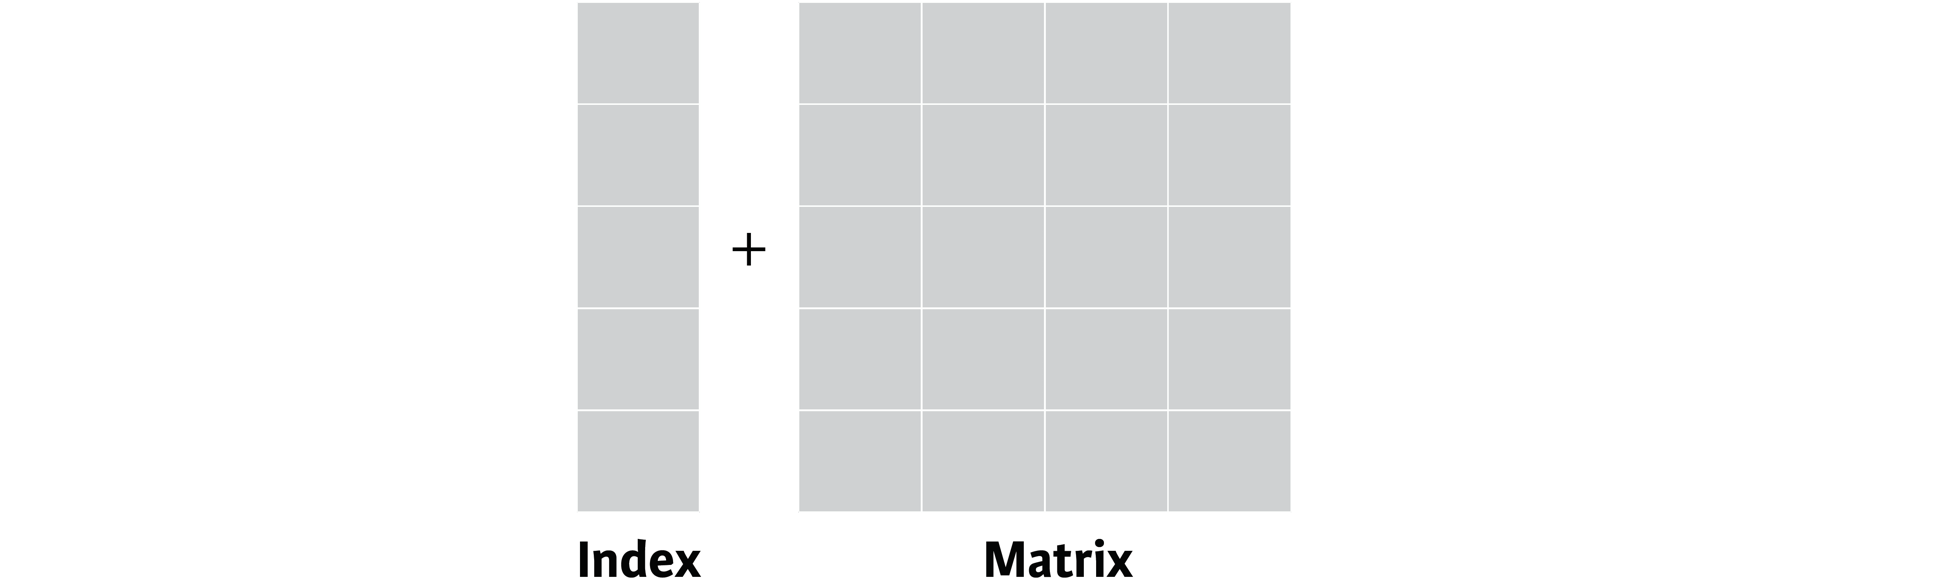
\includegraphics{files/matrixwithindex-wide.png}
\caption{\label{fig:matrix-with-index}Data with Index. \emph{Source}: \href{https://learn.datacamp.com/courses/manipulating-time-series-data-with-xts-and-zoo-in-r}{DataCamp}.}
\end{figure}

The index attached to an \texttt{xts} object is usually a \texttt{Date} or \texttt{POSIXct} vector, maintaining the data in chronological order from earliest to latest. If you wish to sort data (such as stock prices) by another variable (like trade volume), you'll first need to convert the \texttt{xts} object back to a data frame, as \texttt{xts} objects preserve the time order. \texttt{xts} objects are built upon \texttt{zoo} objects (Zeileis' Ordered Observations), another class of time-indexed data structures. \texttt{xts} objects enhance these base structures by providing additional features.

Like \texttt{tibble} and \texttt{data.table}, \texttt{xts} is not included in base R. To use it, you need to install the \texttt{xts} package using \texttt{install.packages("xts")}, then include \texttt{library("xts")} at the start of your script.

To create an \texttt{xts} object, use the \texttt{xts()} function which associates data with a time index (\texttt{order.by\ =\ time\_index}):

\begin{Shaded}
\begin{Highlighting}[]
\CommentTok{\# Load R package}
\FunctionTok{library}\NormalTok{(}\StringTok{"xts"}\NormalTok{)}

\CommentTok{\# Create a new xts object from a matrix:}
\NormalTok{data }\OtherTok{\textless{}{-}} \FunctionTok{matrix}\NormalTok{(}\DecValTok{1}\SpecialCharTok{:}\DecValTok{4}\NormalTok{, }\AttributeTok{ncol =} \DecValTok{2}\NormalTok{, }\AttributeTok{nrow =} \DecValTok{2}\NormalTok{, }\AttributeTok{dimnames =} \FunctionTok{list}\NormalTok{(}\ConstantTok{NULL}\NormalTok{, }\FunctionTok{c}\NormalTok{(}\StringTok{"a"}\NormalTok{, }\StringTok{"b"}\NormalTok{)))}
\NormalTok{data}
\end{Highlighting}
\end{Shaded}

\begin{verbatim}
##      a b
## [1,] 1 3
## [2,] 2 4
\end{verbatim}

\begin{Shaded}
\begin{Highlighting}[]
\NormalTok{time\_index }\OtherTok{\textless{}{-}} \FunctionTok{as.Date}\NormalTok{(}\FunctionTok{c}\NormalTok{(}\StringTok{"2020{-}06{-}01"}\NormalTok{, }\StringTok{"2020{-}07{-}01"}\NormalTok{))}
\NormalTok{time\_index}
\end{Highlighting}
\end{Shaded}

\begin{verbatim}
## [1] "2020-06-01" "2020-07-01"
\end{verbatim}

\begin{Shaded}
\begin{Highlighting}[]
\NormalTok{dxts }\OtherTok{\textless{}{-}} \FunctionTok{xts}\NormalTok{(}\AttributeTok{x =}\NormalTok{ data, }\AttributeTok{order.by =}\NormalTok{ time\_index)}
\NormalTok{dxts}
\end{Highlighting}
\end{Shaded}

\begin{verbatim}
##            a b
## 2020-06-01 1 3
## 2020-07-01 2 4
\end{verbatim}

\begin{Shaded}
\begin{Highlighting}[]
\FunctionTok{class}\NormalTok{(dxts)}
\end{Highlighting}
\end{Shaded}

\begin{verbatim}
## [1] "xts" "zoo"
\end{verbatim}

\begin{Shaded}
\begin{Highlighting}[]
\FunctionTok{tclass}\NormalTok{(dxts)}
\end{Highlighting}
\end{Shaded}

\begin{verbatim}
## [1] "Date"
\end{verbatim}

\begin{Shaded}
\begin{Highlighting}[]
\CommentTok{\# Extract time index}
\FunctionTok{index}\NormalTok{(dxts)}
\end{Highlighting}
\end{Shaded}

\begin{verbatim}
## [1] "2020-06-01" "2020-07-01"
\end{verbatim}

\begin{Shaded}
\begin{Highlighting}[]
\CommentTok{\# Extract data without time index}
\FunctionTok{coredata}\NormalTok{(dxts)}
\end{Highlighting}
\end{Shaded}

\begin{verbatim}
##      a b
## [1,] 1 3
## [2,] 2 4
\end{verbatim}

To delve deeper into \texttt{xts} and \texttt{zoo} objects, consider reading the guides \href{https://rstudio-pubs-static.s3.amazonaws.com/288218_117e183e74964557a5da4fc5902fc671.html}{Manipulating Time Series Data in R with xts \& zoo} and \href{https://rpubs.com/rmariscal/404513}{Time Series in R: Quick Reference}. Additionally, \href{https://learn.datacamp.com/}{DataCamp} provides in-depth courses on these topics:

\begin{itemize}
\tightlist
\item
  \href{https://learn.datacamp.com/courses/manipulating-time-series-data-with-xts-and-zoo-in-r}{Manipulating Time Series Data with xts and zoo in R}
\item
  \href{https://learn.datacamp.com/courses/importing-and-managing-financial-data-in-r}{Importing and Managing Financial Data in R}
\end{itemize}

If you're working within the \texttt{tidyverse} environment, the R package \href{http://www.stats.bris.ac.uk/R/web/packages/tidyquant/vignettes/TQ02-quant-integrations-in-tidyquant.html}{\texttt{tidyquant}} offers seamless integration with \texttt{xts} and \texttt{zoo}. Lastly, this handy \href{https://s3.amazonaws.com/assets.datacamp.com/blog_assets/xts_Cheat_Sheet_R.pdf}{cheat sheet} provides a quick reference on \texttt{xts} and \texttt{zoo} functions.

\hypertarget{importing-data-in-r}{%
\section{Importing Data in R}\label{importing-data-in-r}}

R is a software specialized for data analysis. To analyze data using R, the data must first be imported into the R environment. R offers robust functionality for importing data in a variety of formats. This section explores how to import data from CSV, TSV, and Excel files. Before we dive into specifics, let's ensure RStudio can locate the data stored on your computer.

\hypertarget{working-directory}{%
\subsection{Working Directory}\label{working-directory}}

The working directory in R is the folder where R starts when it's looking for files to read or write. If you're not sure where your current working directory is, you can use the \texttt{getwd()} (get working directory) command in R to find out:

\begin{Shaded}
\begin{Highlighting}[]
\FunctionTok{getwd}\NormalTok{()}
\end{Highlighting}
\end{Shaded}

\begin{verbatim}
## [1] "/Users/julianludwig/Library/CloudStorage/Dropbox/Economics/teaching/4300_2023/module-01"
\end{verbatim}

To change your working directory, use the \texttt{setwd()} (set working directory) function:

\begin{Shaded}
\begin{Highlighting}[]
\FunctionTok{setwd}\NormalTok{(}\StringTok{"your/folder/path"}\NormalTok{)}
\end{Highlighting}
\end{Shaded}

Be sure to replace \texttt{"your/folder/path"} with the actual path to your folder.

When your files are stored in the same directory as your working directory, defined using the \texttt{setwd()} function, you can directly access these files by their names. For instance, \texttt{read\_csv("yieldcurve.csv")} will successfully read the file if ``yieldcurve.csv'' is in the working directory. If the file is located in a subfolder within the working directory, for example a folder named \texttt{files}, you would need to specify the folder in the file path when calling the file: \texttt{read\_csv("files/yieldcurve.csv")}.

To find out the folder path for a specific file or folder on your computer, you can follow these steps:

\hypertarget{for-windows-1}{%
\subsubsection*{For Windows:}\label{for-windows-1}}
\addcontentsline{toc}{subsubsection}{For Windows:}

\begin{enumerate}
\def\labelenumi{\arabic{enumi}.}
\tightlist
\item
  Navigate to the folder using the File Explorer.
\item
  Once you are in the folder, click on the address bar at the top of the File Explorer window. The address bar will now show the full path to the folder. This is the path you can set in R using the \texttt{setwd()} function.
\end{enumerate}

An example of a folder path on Windows might look like this: \texttt{C:/Users/YourName/Documents/R}.

\hypertarget{for-macos-1}{%
\subsubsection*{For MacOS:}\label{for-macos-1}}
\addcontentsline{toc}{subsubsection}{For MacOS:}

\begin{enumerate}
\def\labelenumi{\arabic{enumi}.}
\tightlist
\item
  Open Finder and navigate to the folder.
\item
  Once you are in the folder, Command-click (or right-click and hold, if you have a mouse) on the folder's name at the top of the Finder window. A drop-down menu will appear showing the folder hierarchy.
\item
  Hover over each folder in the hierarchy to show the full path, then copy this path.
\end{enumerate}

An example of a folder path on macOS might look like this: \texttt{/Users/YourName/Documents/R}.

Remember, when setting the working directory in R, you need to use forward slashes (\texttt{/}) in the folder path, even on Windows where the convention is to use backslashes (\texttt{\textbackslash{}}).

\hypertarget{csv-comma-separated-values}{%
\subsection{CSV (Comma Separated Values)}\label{csv-comma-separated-values}}

CSV (Comma Separated Values) is a common file format used to store tabular data. As the name suggests, the values in each row of a CSV file are separated by commas. Here's an example of how data is stored in a CSV file:

\begin{itemize}
\tightlist
\item
  Male,8,100,3
\item
  Female,9,20,3
\end{itemize}

In this section, we'll demonstrate how to import a CSV file using real-world Treasury yield curve rates data.

\hypertarget{import-yield-curve-data-in-csv-format}{%
\subsubsection*{Import Yield Curve Data in CSV Format}\label{import-yield-curve-data-in-csv-format}}
\addcontentsline{toc}{subsubsection}{Import Yield Curve Data in CSV Format}

To obtain the yield curve data, follow these steps:

\begin{enumerate}
\def\labelenumi{\arabic{enumi}.}
\tightlist
\item
  Visit the U.S. Treasury's data center by clicking \href{https://www.treasury.gov/resource-center/data-chart-center}{here}.
\item
  Click on ``Data'' in the menu bar, then select ``Daily Treasury Par Yield Curve Rates.''
\item
  On the data page, select ``Download CSV'' to obtain the yield curve data for the current year.
\item
  To access all the yield curve data since 1990, choose ``All'' under the ``Select Time Period'' option, and click ``Apply.'' Please note that when selecting all periods, the ``Download CSV'' button may not be available.
\item
  To manually save the data as a CSV file, you can copy the data by selecting it and using the Ctrl+C (or Cmd+C) command. Open an Excel file, and use the Ctrl+V (or Cmd+V) command to paste the data into the Excel file.
\item
  Save the Excel file as a CSV file named `yieldcurve.csv' in a location of your choice, ensuring that it is saved in a familiar folder for easy access.
\end{enumerate}

Next, install and load the \texttt{readr} package. Run \texttt{install.packages("readr")} in the console and include the package at the top of your R script. You can then use the \texttt{read\_csv()} or \texttt{read\_delim()} function to import the yield curve data:

\begin{Shaded}
\begin{Highlighting}[]
\CommentTok{\# Load the package}
\FunctionTok{library}\NormalTok{(}\StringTok{"readr"}\NormalTok{)}

\CommentTok{\# Import CSV file}
\NormalTok{yc }\OtherTok{\textless{}{-}} \FunctionTok{read\_csv}\NormalTok{(}\AttributeTok{file =} \StringTok{"files/yieldcurve.csv"}\NormalTok{, }\AttributeTok{col\_names =} \ConstantTok{TRUE}\NormalTok{)}
\end{Highlighting}
\end{Shaded}

\begin{verbatim}
## Warning: One or more parsing issues, call `problems()` on your data frame for details,
## e.g.:
##   dat <- vroom(...)
##   problems(dat)
\end{verbatim}

\begin{verbatim}
## Rows: 8382 Columns: 14
## -- Column specification --------------------------------------------------------
## Delimiter: ","
## chr (6): Date, 1 Mo, 2 Mo, 4 Mo, 20 Yr, 30 Yr
## dbl (8): 3 Mo, 6 Mo, 1 Yr, 2 Yr, 3 Yr, 5 Yr, 7 Yr, 10 Yr
## 
## i Use `spec()` to retrieve the full column specification for this data.
## i Specify the column types or set `show_col_types = FALSE` to quiet this message.
\end{verbatim}

\begin{Shaded}
\begin{Highlighting}[]
\CommentTok{\# Import CSV file using the read\_delim() function}
\NormalTok{yc }\OtherTok{\textless{}{-}} \FunctionTok{read\_delim}\NormalTok{(}\AttributeTok{file =} \StringTok{"files/yieldcurve.csv"}\NormalTok{, }\AttributeTok{col\_names =} \ConstantTok{TRUE}\NormalTok{, }\AttributeTok{delim =} \StringTok{","}\NormalTok{)}
\end{Highlighting}
\end{Shaded}

\begin{verbatim}
## Warning: One or more parsing issues, call `problems()` on your data frame for details,
## e.g.:
##   dat <- vroom(...)
##   problems(dat)
\end{verbatim}

\begin{verbatim}
## Rows: 8382 Columns: 14
## -- Column specification --------------------------------------------------------
## Delimiter: ","
## chr (6): Date, 1 Mo, 2 Mo, 4 Mo, 20 Yr, 30 Yr
## dbl (8): 3 Mo, 6 Mo, 1 Yr, 2 Yr, 3 Yr, 5 Yr, 7 Yr, 10 Yr
## 
## i Use `spec()` to retrieve the full column specification for this data.
## i Specify the column types or set `show_col_types = FALSE` to quiet this message.
\end{verbatim}

In the code snippets above, the \texttt{read\_csv()} and \texttt{read\_delim()} functions from the \texttt{readr} package are used to import a CSV file named ``yieldcurve.csv''. The \texttt{col\_names\ =\ TRUE} argument indicates that the first row of the CSV file contains column names. The \texttt{delim\ =\ ","} argument specifies that the columns are separated by commas, which is the standard delimiter for CSV (\emph{Comma} Separated Values) files. Either one of the two functions can be used to read the CSV file and store the data in the variable \texttt{yc} for further analysis.

To inspect the first few rows of the data, print the \texttt{yc} object in the console. For an overview of the entire dataset, use the \texttt{View()} function, which provides an interface similar to viewing the CSV file in Microsoft Excel:

\begin{Shaded}
\begin{Highlighting}[]
\CommentTok{\# Display the data}
\NormalTok{yc}
\end{Highlighting}
\end{Shaded}

\begin{verbatim}
## # A tibble: 8,382 x 14
##    Date    `1 Mo` `2 Mo` `3 Mo` `4 Mo` `6 Mo` `1 Yr` `2 Yr` `3 Yr` `5 Yr` `7 Yr`
##    <chr>   <chr>  <chr>   <dbl> <chr>   <dbl>  <dbl>  <dbl>  <dbl>  <dbl>  <dbl>
##  1 01/02/~ N/A    N/A      7.83 N/A      7.89   7.81   7.87   7.9    7.87   7.98
##  2 01/03/~ N/A    N/A      7.89 N/A      7.94   7.85   7.94   7.96   7.92   8.04
##  3 01/04/~ N/A    N/A      7.84 N/A      7.9    7.82   7.92   7.93   7.91   8.02
##  4 01/05/~ N/A    N/A      7.79 N/A      7.85   7.79   7.9    7.94   7.92   8.03
##  5 01/08/~ N/A    N/A      7.79 N/A      7.88   7.81   7.9    7.95   7.92   8.05
##  6 01/09/~ N/A    N/A      7.8  N/A      7.82   7.78   7.91   7.94   7.92   8.05
##  7 01/10/~ N/A    N/A      7.75 N/A      7.78   7.77   7.91   7.95   7.92   8   
##  8 01/11/~ N/A    N/A      7.8  N/A      7.8    7.77   7.91   7.95   7.94   8.01
##  9 01/12/~ N/A    N/A      7.74 N/A      7.81   7.76   7.93   7.98   7.99   8.07
## 10 01/16/~ N/A    N/A      7.89 N/A      7.99   7.92   8.1    8.13   8.11   8.18
## # i 8,372 more rows
## # i 3 more variables: `10 Yr` <dbl>, `20 Yr` <chr>, `30 Yr` <chr>
\end{verbatim}

\begin{Shaded}
\begin{Highlighting}[]
\CommentTok{\# Display the data in a spreadsheet{-}like format}
\FunctionTok{View}\NormalTok{(yc)}
\end{Highlighting}
\end{Shaded}

Both the \texttt{read\_csv()} and \texttt{read\_delim()} functions convert the CSV file into a tibble (\texttt{tbl\_df}), a modern version of the R data frame discussed in Section \ref{tibble}. Remember, a data frame stores data in separate columns, each of which must be of the same data type. Use the \texttt{class(yc)} function to check the data type of the entire dataset, and \texttt{sapply(yc,\ class)} to check the data type of each column:

\begin{Shaded}
\begin{Highlighting}[]
\CommentTok{\# Check the data type of the entire dataset}
\FunctionTok{class}\NormalTok{(yc)}
\end{Highlighting}
\end{Shaded}

\begin{verbatim}
## [1] "spec_tbl_df" "tbl_df"      "tbl"         "data.frame"
\end{verbatim}

\begin{Shaded}
\begin{Highlighting}[]
\CommentTok{\# Check the data type of each column}
\FunctionTok{sapply}\NormalTok{(yc, class)}
\end{Highlighting}
\end{Shaded}

\begin{verbatim}
##        Date        1 Mo        2 Mo        3 Mo        4 Mo        6 Mo 
## "character" "character" "character"   "numeric" "character"   "numeric" 
##        1 Yr        2 Yr        3 Yr        5 Yr        7 Yr       10 Yr 
##   "numeric"   "numeric"   "numeric"   "numeric"   "numeric"   "numeric" 
##       20 Yr       30 Yr 
## "character" "character"
\end{verbatim}

When importing data in R, it's possible that R assigns incorrect data types to some columns. For example, the \texttt{Date} column is treated as a character column even though it contains dates, and the \texttt{30\ Yr} column is treated as a character column even though it contains interest rates. To address this issue, you can convert the first column to a date type and the remaining columns to numeric data types using the following three steps:

\begin{enumerate}
\def\labelenumi{\arabic{enumi}.}
\tightlist
\item
  Replace ``N/A'' with \texttt{NA}, which represents missing values in R. This step is necessary because R doesn't recognize ``N/A'', and if a column includes ``N/A'', R will consider it as a character vector instead of a numeric vector.
\end{enumerate}

\begin{Shaded}
\begin{Highlighting}[]
\NormalTok{yc[yc }\SpecialCharTok{==} \StringTok{"N/A"}\NormalTok{] }\OtherTok{\textless{}{-}} \ConstantTok{NA}
\end{Highlighting}
\end{Shaded}

\begin{enumerate}
\def\labelenumi{\arabic{enumi}.}
\setcounter{enumi}{1}
\tightlist
\item
  Convert all yield columns to numeric data types:
\end{enumerate}

\begin{Shaded}
\begin{Highlighting}[]
\NormalTok{yc[, }\SpecialCharTok{{-}}\DecValTok{1}\NormalTok{] }\OtherTok{\textless{}{-}} \FunctionTok{sapply}\NormalTok{(yc[, }\SpecialCharTok{{-}}\DecValTok{1}\NormalTok{], as.numeric)}
\end{Highlighting}
\end{Shaded}

The \texttt{as.numeric()} function converts a data object into a numeric type. In this case, it converts columns with character values like ``3'' and ``4'' into the numeric values 3 and 4. The \texttt{sapply()} function applies the \texttt{as.numeric()} function to each of the selected columns. This converts all the interest rates to numeric data types.

\begin{enumerate}
\def\labelenumi{\arabic{enumi}.}
\setcounter{enumi}{2}
\tightlist
\item
  Convert the date column to a date object, recognizing that the date format is Month/Day/Year or \texttt{\%m/\%d/\%Y}:
\end{enumerate}

\begin{Shaded}
\begin{Highlighting}[]
\CommentTok{\# Check the date format}
\FunctionTok{head}\NormalTok{(yc}\SpecialCharTok{$}\NormalTok{Date)}
\end{Highlighting}
\end{Shaded}

\begin{verbatim}
## [1] "01/02/1990" "01/03/1990" "01/04/1990" "01/05/1990" "01/08/1990"
## [6] "01/09/1990"
\end{verbatim}

\begin{Shaded}
\begin{Highlighting}[]
\CommentTok{\# Convert to date format}
\NormalTok{yc}\SpecialCharTok{$}\NormalTok{Date }\OtherTok{\textless{}{-}} \FunctionTok{as.Date}\NormalTok{(yc}\SpecialCharTok{$}\NormalTok{Date, }\AttributeTok{format =} \StringTok{"\%m/\%d/\%Y"}\NormalTok{)}
\FunctionTok{head}\NormalTok{(yc}\SpecialCharTok{$}\NormalTok{Date)}
\end{Highlighting}
\end{Shaded}

\begin{verbatim}
## [1] "1990-01-02" "1990-01-03" "1990-01-04" "1990-01-05" "1990-01-08"
## [6] "1990-01-09"
\end{verbatim}

Hence, we have successfully imported the yield curve data and performed the necessary conversions to ensure that all columns are in their correct formats:

\begin{Shaded}
\begin{Highlighting}[]
\NormalTok{yc}
\end{Highlighting}
\end{Shaded}

\begin{verbatim}
## # A tibble: 8,382 x 14
##    Date       `1 Mo` `2 Mo` `3 Mo` `4 Mo` `6 Mo` `1 Yr` `2 Yr` `3 Yr` `5 Yr`
##    <date>      <dbl>  <dbl>  <dbl>  <dbl>  <dbl>  <dbl>  <dbl>  <dbl>  <dbl>
##  1 1990-01-02     NA     NA   7.83     NA   7.89   7.81   7.87   7.9    7.87
##  2 1990-01-03     NA     NA   7.89     NA   7.94   7.85   7.94   7.96   7.92
##  3 1990-01-04     NA     NA   7.84     NA   7.9    7.82   7.92   7.93   7.91
##  4 1990-01-05     NA     NA   7.79     NA   7.85   7.79   7.9    7.94   7.92
##  5 1990-01-08     NA     NA   7.79     NA   7.88   7.81   7.9    7.95   7.92
##  6 1990-01-09     NA     NA   7.8      NA   7.82   7.78   7.91   7.94   7.92
##  7 1990-01-10     NA     NA   7.75     NA   7.78   7.77   7.91   7.95   7.92
##  8 1990-01-11     NA     NA   7.8      NA   7.8    7.77   7.91   7.95   7.94
##  9 1990-01-12     NA     NA   7.74     NA   7.81   7.76   7.93   7.98   7.99
## 10 1990-01-16     NA     NA   7.89     NA   7.99   7.92   8.1    8.13   8.11
## # i 8,372 more rows
## # i 4 more variables: `7 Yr` <dbl>, `10 Yr` <dbl>, `20 Yr` <dbl>, `30 Yr` <dbl>
\end{verbatim}

Here, \texttt{\textless{}dbl\textgreater{}} stands for double, which is the R data type for decimal numbers, also known as numeric type. Converting the yield columns to \texttt{dbl} ensures that the values are treated as numeric and can be used for calculations, analysis, and visualization.

\hypertarget{plot-historical-trends-in-treasury-yields}{%
\subsubsection*{Plot Historical Trends in Treasury Yields}\label{plot-historical-trends-in-treasury-yields}}
\addcontentsline{toc}{subsubsection}{Plot Historical Trends in Treasury Yields}

Let's use the \texttt{plot()} function to visualize the imported yield curve data. In this case, we will plot the 3-month Treasury rate over time, using the \texttt{Date} column as the x-axis and the \texttt{3\ Mo} column as the y-axis:

\begin{Shaded}
\begin{Highlighting}[]
\CommentTok{\# Plot the 3{-}month Treasury rate over time}
\FunctionTok{plot}\NormalTok{(}\AttributeTok{x =}\NormalTok{ yc}\SpecialCharTok{$}\NormalTok{Date, }\AttributeTok{y =}\NormalTok{ yc}\SpecialCharTok{$}\StringTok{\textasciigrave{}}\AttributeTok{3 Mo}\StringTok{\textasciigrave{}}\NormalTok{, }\AttributeTok{type =} \StringTok{"l"}\NormalTok{,}
     \AttributeTok{xlab =} \StringTok{"Date"}\NormalTok{, }\AttributeTok{ylab =} \StringTok{"\%"}\NormalTok{, }\AttributeTok{main =} \StringTok{"3{-}Month Treasury Rate"}\NormalTok{)}
\end{Highlighting}
\end{Shaded}

In the code snippet above, \texttt{plot()} is the R function used to create the plot. It takes several arguments to customize the appearance and behavior of the plot:

\begin{itemize}
\tightlist
\item
  \texttt{x} represents the data to be plotted on the x-axis. In this case, it corresponds to the \texttt{Date} column from the yield curve data.
\item
  \texttt{y} represents the data to be plotted on the y-axis. Here, it corresponds to the \texttt{3\ Mo} column, which represents the 3-month Treasury rate.
\item
  \texttt{type\ =\ "l"} specifies the type of plot to create. In this case, we use \texttt{"l"} to create a line plot.
\item
  \texttt{xlab\ =\ "Date"} sets the label for the x-axis to ``Date''.
\item
  \texttt{ylab\ =\ "\%"} sets the label for the y-axis to ``\%''.
\item
  \texttt{main\ =\ "3-Month\ Treasury\ Rate"} sets the title of the plot to ``3-Month Treasury Rate''.
\end{itemize}

\begin{figure}
\centering
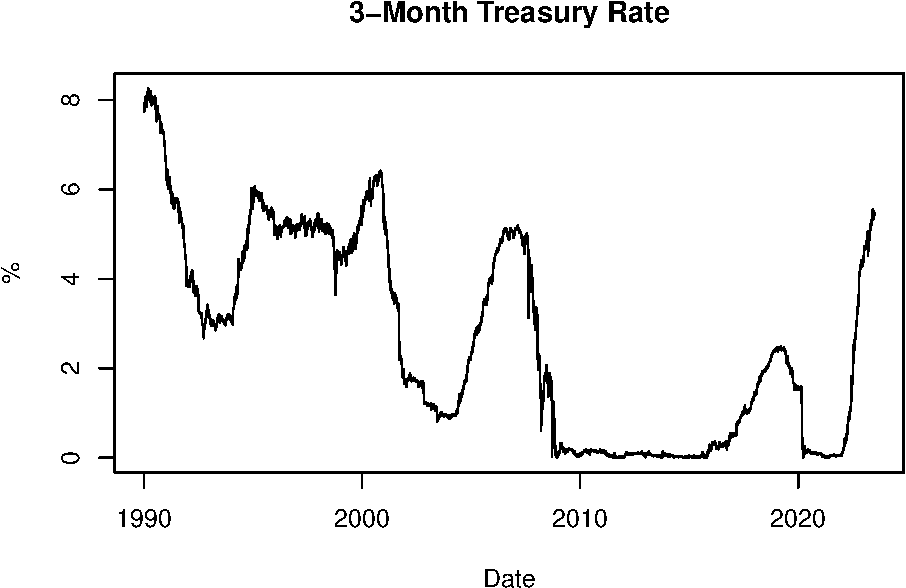
\includegraphics{_main_files/figure-latex/yield-historical-plot-1.pdf}
\caption{\label{fig:yield-historical-plot}3-Month Treasury Rate}
\end{figure}

The resulting plot, shown in Figure \ref{fig:yield-historical-plot}, displays the historical evolution of the 3-month Treasury rate since 1990. It allows us to observe how interest rates have changed over time, with low rates often observed during recessions and high rates during boom periods. Recessions are typically characterized by reduced borrowing and investment activities, leading to decreased demand for credit and lower interest rates. Conversely, boom periods are associated with strong economic growth and increased credit demand, which can drive interest rates upward.

Furthermore, inflation plays a significant role in influencing interest rates through the Fisher effect. When inflation is high, lenders and investors are concerned about the diminishing value of money over time. To compensate for the erosion of purchasing power, lenders typically demand higher interest rates on loans. These higher interest rates reflect the expectation of future inflation and act as a safeguard against the declining value of the money lent. Conversely, when inflation is low, lenders may offer lower interest rates due to reduced concerns about the erosion of purchasing power.

\hypertarget{plot-yield-curve}{%
\subsubsection*{Plot Yield Curve}\label{plot-yield-curve}}
\addcontentsline{toc}{subsubsection}{Plot Yield Curve}

Next, let's plot the yield curve. The yield curve is a graphical representation of the relationship between the interest rates (yields) and the time to maturity of a bond. It provides insights into market expectations regarding future interest rates and economic conditions.

To plot the yield curve, we will select the most recently available data from the dataset, which corresponds to the last row. We will extract the interest rates as a numeric vector and the column names (representing the time to maturity) as labels for the x-axis:

\begin{Shaded}
\begin{Highlighting}[]
\CommentTok{\# Extract the interest rates of the last row}
\NormalTok{yc\_most\_recent\_data }\OtherTok{\textless{}{-}} \FunctionTok{as.numeric}\NormalTok{(}\FunctionTok{last}\NormalTok{(yc[, }\SpecialCharTok{{-}}\DecValTok{1}\NormalTok{]))}
\NormalTok{yc\_most\_recent\_data}
\end{Highlighting}
\end{Shaded}

\begin{verbatim}
##  [1] 5.24 5.39 5.43 5.50 5.47 5.40 4.87 4.49 4.13 3.97 3.81 4.06 3.85
\end{verbatim}

\begin{Shaded}
\begin{Highlighting}[]
\CommentTok{\# Extract the column names of the last row}
\NormalTok{yc\_most\_recent\_labels }\OtherTok{\textless{}{-}} \FunctionTok{colnames}\NormalTok{(}\FunctionTok{last}\NormalTok{(yc[, }\SpecialCharTok{{-}}\DecValTok{1}\NormalTok{]))}
\NormalTok{yc\_most\_recent\_labels}
\end{Highlighting}
\end{Shaded}

\begin{verbatim}
##  [1] "1 Mo"  "2 Mo"  "3 Mo"  "4 Mo"  "6 Mo"  "1 Yr"  "2 Yr"  "3 Yr"  "5 Yr" 
## [10] "7 Yr"  "10 Yr" "20 Yr" "30 Yr"
\end{verbatim}

\begin{Shaded}
\begin{Highlighting}[]
\CommentTok{\# Plot the yield curve}
\FunctionTok{plot}\NormalTok{(}\AttributeTok{x =}\NormalTok{ yc\_most\_recent\_data, }\AttributeTok{xaxt =} \StringTok{\textquotesingle{}n\textquotesingle{}}\NormalTok{, }\AttributeTok{type =} \StringTok{"o"}\NormalTok{, }\AttributeTok{pch =} \DecValTok{19}\NormalTok{,}
     \AttributeTok{xlab =} \StringTok{"Time to Maturity"}\NormalTok{, }\AttributeTok{ylab =} \StringTok{"Treasury Rate in \%"}\NormalTok{,}
     \AttributeTok{main =} \FunctionTok{paste}\NormalTok{(}\StringTok{"Yield Curve on"}\NormalTok{, }\FunctionTok{format}\NormalTok{(}\FunctionTok{last}\NormalTok{(yc}\SpecialCharTok{$}\NormalTok{Date), }\AttributeTok{format =} \StringTok{\textquotesingle{}\%B \%d, \%Y\textquotesingle{}}\NormalTok{)))}
\FunctionTok{axis}\NormalTok{(}\AttributeTok{side =} \DecValTok{1}\NormalTok{, }\AttributeTok{at =} \FunctionTok{seq}\NormalTok{(}\DecValTok{1}\NormalTok{, }\FunctionTok{length}\NormalTok{(yc\_most\_recent\_labels), }\DecValTok{1}\NormalTok{), }
     \AttributeTok{labels =}\NormalTok{ yc\_most\_recent\_labels)}
\end{Highlighting}
\end{Shaded}

In the code snippet above, \texttt{plot()} is the R function used to create the yield curve plot. Here are the key inputs and arguments used in the function:

\begin{itemize}
\tightlist
\item
  \texttt{x\ =\ yc\_most\_recent\_data} represents the interest rates of the most recent yield curve data, which will be plotted on the x-axis.
\item
  \texttt{xaxt\ =\ \textquotesingle{}n\textquotesingle{}} specifies that no x-axis tick labels should be displayed initially. This is useful because we will customize the x-axis tick labels separately using the \texttt{axis()} function.
\item
  \texttt{type\ =\ "o"} specifies that the plot should be created as a line plot with points. This will display the yield curve as a connected line with markers at each data point.
\item
  \texttt{pch\ =\ 19} sets the plot symbol to a solid circle, which will be used as markers for the data points on the yield curve.
\item
  \texttt{xlab\ =\ "Time\ to\ Maturity"} sets the label for the x-axis to ``Time to Maturity'', indicating the variable represented on the x-axis.
\item
  \texttt{ylab\ =\ "Treasury\ Rate\ in\ \%"} sets the label for the y-axis to ``Treasury Rate in \%'', indicating the variable represented on the y-axis.
\item
  \texttt{main\ =\ paste("Yield\ Curve\ on",\ format(last(yc\$Date),\ format\ =\ \textquotesingle{}\%B\ \%d,\ \%Y\textquotesingle{}))} sets the title of the plot to ``Yield Curve on'' followed by the date of the most recent yield curve data.
\end{itemize}

Additionally, the \texttt{axis()} function is used to customize the x-axis tick labels. It sets the tick locations using \texttt{at\ =\ seq(1,\ length(yc\_most\_recent\_labels),\ 1)} to evenly space the ticks along the x-axis. The \texttt{labels\ =\ yc\_most\_recent\_labels} argument assigns the column names of the last row (representing maturities) as the tick labels on the x-axis.

\begin{figure}
\centering
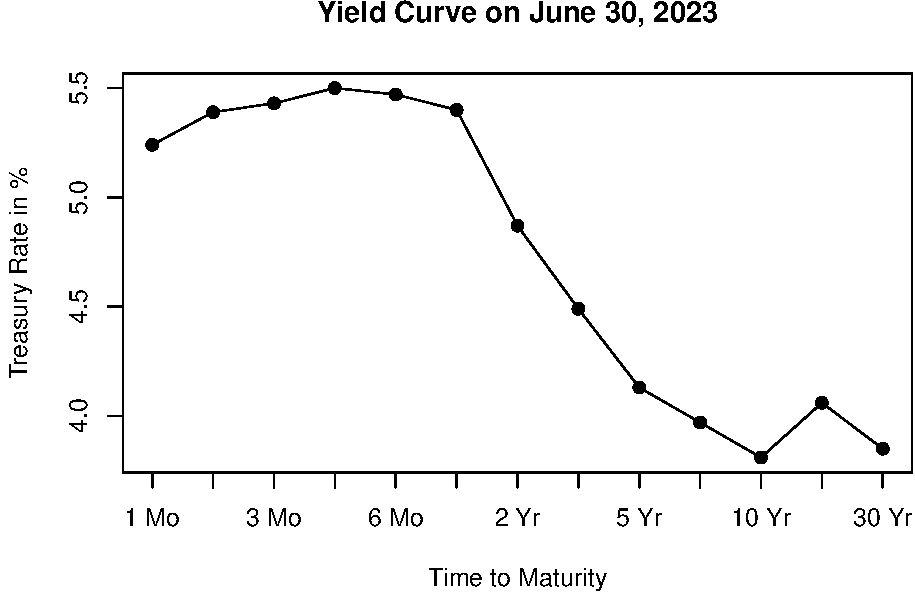
\includegraphics{_main_files/figure-latex/yield-curve-plot-1.pdf}
\caption{\label{fig:yield-curve-plot}Yield Curve on June 30, 2023}
\end{figure}

The resulting plot, shown in Figure \ref{fig:yield-curve-plot}, depicts the yield curve based on the most recent available data, allowing us to visualize the relationship between interest rates and the time to maturity. The x-axis represents the different maturities of the bonds, while the y-axis represents the corresponding treasury rates.

Analyzing the shape of the yield curve can provide insights into market expectations and can be useful for assessing economic conditions and making investment decisions. The yield curve can take different shapes, such as upward-sloping (normal), downward-sloping (inverted), or flat, each indicating different market conditions and expectations for future interest rates.

An upward-sloping yield curve, where longer-term interest rates are higher than shorter-term rates, is often seen during periods of economic expansion. This shape suggests that investors expect higher interest rates in the future as the economy grows and inflationary pressures increase. It reflects an optimistic outlook for economic conditions, as borrowing and lending activity are expected to be robust.

In contrast, a downward-sloping or inverted yield curve, where shorter-term interest rates are higher than longer-term rates, is often considered a predictor of economic slowdown or recession. This shape suggests that investors anticipate lower interest rates in the future as economic growth slows and inflationary pressures decrease. It reflects a more cautious outlook for the economy, as investors seek the safety of longer-term bonds amid expectations of lower returns and potential economic downturn.

Inflation expectations also influence the shape of the yield curve. When there are high inflation expectations for the long term, the yield curve tends to slope upwards. This occurs because lenders demand higher interest rates for longer maturities to compensate for anticipated inflation. However, when there is currently high inflation but expectations are that the central bank will successfully control inflation in the long term, the yield curve may slope downwards. In this case, long-term interest rates are lower than short-term rates, as average inflation over the long term is expected to be lower than in the short term.

\hypertarget{tsv-tab-separated-values}{%
\subsection{TSV (Tab Separated Values)}\label{tsv-tab-separated-values}}

TSV (Tab Separated Values) is a common file format used to store tabular data. As the name suggests, the values in each row of a TSV file are separated by tabs. Here's an example of how data is stored in a TSV file:

\begin{itemize}
\tightlist
\item
  Male~~~~8~~~~100~~~~3
\item
  Female~~~~9~~~~20~~~~3
\end{itemize}

In this section, we'll demonstrate how to import a TSV file using real-world consumer survey data collected by the University of Michigan.

\hypertarget{import-michigan-consumer-survey-data-in-tsv-format}{%
\subsubsection*{Import Michigan Consumer Survey Data in TSV Format}\label{import-michigan-consumer-survey-data-in-tsv-format}}
\addcontentsline{toc}{subsubsection}{Import Michigan Consumer Survey Data in TSV Format}

To obtain the Michigan consumer survey data, follow these steps:

\begin{enumerate}
\def\labelenumi{\arabic{enumi}.}
\tightlist
\item
  Visit the website of University of Michigan's surveys of consumers by clicking \href{https://data.sca.isr.umich.edu/}{here}.
\item
  Click on ``DATA'' in the menu bar, then select ``Time Series.''
\item
  On the data page, under Table, select ``All: All Tables (Tab-delimited or CSV only)'' to obtain the consumer survey data on all topics.
\item
  To access all the consumer survey data since 1978, type ``1978'' under the ``Oldest Year'' option.
\item
  Click on ``Tab-Deliminated (Excel)'' under the ``format'' option.
\item
  Save the TSV file in a location of your choice, ensuring that it is saved in a familiar folder for easy access.
\end{enumerate}

The dataset contains 360 variables with coded column names such as \texttt{ics\_inc31} or \texttt{pago\_dk\_all}. To understand the meaning of these columns, you can visit the same website \href{https://data.sca.isr.umich.edu/}{here} and click on \href{https://data.sca.isr.umich.edu/survey-info.php\#}{SURVEY INFORMATION}. From there, select the \href{https://data.sca.isr.umich.edu/fetchdoc.php?docid=45121}{Time-Series Variable Codebook} which is a PDF document that provides detailed explanations for all the column names. By referring to this codebook, you can gain a better understanding of the variables and their corresponding meanings in the dataset.

Next, to import the consumer survey data, you need to install and load the \texttt{readr} package if you haven't done so already. Once the package is loaded, you can use either the \texttt{read\_tsv()} or \texttt{read\_delim()} function to read the TSV (Tab-Separated Values) file.

\begin{Shaded}
\begin{Highlighting}[]
\CommentTok{\# Load the package}
\FunctionTok{library}\NormalTok{(}\StringTok{"readr"}\NormalTok{)}

\CommentTok{\# Import TSV file}
\NormalTok{cs }\OtherTok{\textless{}{-}} \FunctionTok{read\_tsv}\NormalTok{(}\AttributeTok{file =} \StringTok{"files/sca{-}tableall{-}on{-}2023{-}Jul{-}01.tsv"}\NormalTok{, }\AttributeTok{skip =} \DecValTok{1}\NormalTok{)}
\end{Highlighting}
\end{Shaded}

\begin{verbatim}
## New names:
## Rows: 545 Columns: 360
## -- Column specification
## -------------------------------------------------------- Delimiter: "\t" dbl
## (359): Month, yyyy, ics_all, ics_inc31, ics_inc32, ics_inc33, ics_a1834,... lgl
## (1): ...360
## i Use `spec()` to retrieve the full column specification for this data. i
## Specify the column types or set `show_col_types = FALSE` to quiet this message.
## * `` -> `...360`
\end{verbatim}

\begin{Shaded}
\begin{Highlighting}[]
\CommentTok{\# Import TSV file using the read\_delim() function}
\NormalTok{cs }\OtherTok{\textless{}{-}} \FunctionTok{read\_delim}\NormalTok{(}\AttributeTok{file =} \StringTok{"files/sca{-}tableall{-}on{-}2023{-}Jul{-}01.tsv"}\NormalTok{, }\AttributeTok{skip =} \DecValTok{1}\NormalTok{, }\AttributeTok{col\_names =} \ConstantTok{TRUE}\NormalTok{, }\AttributeTok{delim =} \StringTok{"}\SpecialCharTok{\textbackslash{}t}\StringTok{"}\NormalTok{)}
\end{Highlighting}
\end{Shaded}

\begin{verbatim}
## New names:
## Rows: 545 Columns: 360
## -- Column specification
## -------------------------------------------------------- Delimiter: "\t" dbl
## (359): Month, yyyy, ics_all, ics_inc31, ics_inc32, ics_inc33, ics_a1834,... lgl
## (1): ...360
## i Use `spec()` to retrieve the full column specification for this data. i
## Specify the column types or set `show_col_types = FALSE` to quiet this message.
## * `` -> `...360`
\end{verbatim}

In the provided code snippets, the \texttt{file} input specifies the file path or URL of the TSV file to be imported. The \texttt{skip} input is used to specify the number of rows to skip at the beginning of the file. In this case, \texttt{skip\ =\ 1} indicates that the first line of the TSV file, which contains the title ``All Tables'', should be skipped. The \texttt{col\_names} input is set to \texttt{TRUE} to indicate that the second line of the TSV file (after skipping 1 row) contains the column names. Lastly, the \texttt{delim} input is set to \texttt{"\textbackslash{}t"} to specify that the columns in the TSV file are separated by tabs, which is the standard delimiter for TSV (\emph{Tab} Separated Values) files.

Note that if the file is neither CSV nor TSV, but rather has an exotic format where columns are separated by a different character that is neither a comma nor a tab, such as ``/'', you can use the \texttt{read\_delim()} function with the \texttt{delim\ =\ "/"} argument to specify the custom delimiter.

To inspect the first few rows of the data, print the \texttt{cs} object in the console. For an overview of the entire dataset, execute \texttt{View(cs)}.

\begin{Shaded}
\begin{Highlighting}[]
\CommentTok{\# Display the data}
\NormalTok{cs}
\end{Highlighting}
\end{Shaded}

\begin{verbatim}
## # A tibble: 545 x 360
##    Month  yyyy ics_all ics_inc31 ics_inc32 ics_inc33 ics_a1834 ics_a3554
##    <dbl> <dbl>   <dbl>     <dbl>     <dbl>     <dbl>     <dbl>     <dbl>
##  1     1  1978    83.7        NA        NA        NA      93.7      86.7
##  2     2  1978    84.3        NA        NA        NA      99.7      82.3
##  3     3  1978    78.8        NA        NA        NA      91.7      76.8
##  4     4  1978    81.6        NA        NA        NA      91.8      79.7
##  5     5  1978    82.9        NA        NA        NA      95.1      78.9
##  6     6  1978    80          NA        NA        NA      91.7      75.7
##  7     7  1978    82.4        NA        NA        NA      92.2      78.4
##  8     8  1978    78.4        NA        NA        NA      87.8      77.2
##  9     9  1978    80.4        NA        NA        NA      86.6      83.9
## 10    10  1978    79.3        NA        NA        NA      90.6      76.7
## # i 535 more rows
## # i 352 more variables: ics_a5597 <dbl>, ics_ne <dbl>, ics_nc <dbl>,
## #   ics_s <dbl>, ics_w <dbl>, icc_all <dbl>, ice_all <dbl>, pago_f_all <dbl>,
## #   pago_s_all <dbl>, pago_u_all <dbl>, pago_dk_all <dbl>, pago_r_all <dbl>,
## #   pagorn_hy_all <dbl>, pagorn_ha_all <dbl>, pagorn_ld_all <dbl>,
## #   pagorn_ly_all <dbl>, pagorn_hp_all <dbl>, pagorn_la_all <dbl>,
## #   pagorn_hd_all <dbl>, pagorn_ny_all <dbl>, pagorn_nad_all <dbl>, ...
\end{verbatim}

Use \texttt{sapply(cs,\ class)} to check the data type of each column, to make sure all columns are indeed numeric:

\begin{Shaded}
\begin{Highlighting}[]
\CommentTok{\# Check the data type of each column}
\FunctionTok{table}\NormalTok{(}\FunctionTok{sapply}\NormalTok{(cs, class))}
\end{Highlighting}
\end{Shaded}

\begin{verbatim}
## 
## logical numeric 
##       1     359
\end{verbatim}

Here, since there are 360 columns, the \texttt{summary()} function is applied, which reveals that there are 359 numerical columns, and 1 logical column, which makes sense.

Instead of a date column, the consumer survey has a year (\texttt{yyyy}) and a month (\texttt{Month}) column. To create a date column from the year and month columns, combine them with the \texttt{paste()} function to create a date format of the form Year-Month-Day or \texttt{\%Y-\%m-\%d}:

\begin{Shaded}
\begin{Highlighting}[]
\CommentTok{\# Create date column}
\NormalTok{cs}\SpecialCharTok{$}\NormalTok{Date }\OtherTok{\textless{}{-}} \FunctionTok{as.Date}\NormalTok{(}\FunctionTok{paste}\NormalTok{(cs}\SpecialCharTok{$}\NormalTok{yyyy, cs}\SpecialCharTok{$}\NormalTok{Month, }\StringTok{"01"}\NormalTok{, }\AttributeTok{sep =} \StringTok{"{-}"}\NormalTok{))}
\FunctionTok{head}\NormalTok{(cs}\SpecialCharTok{$}\NormalTok{Date)}
\end{Highlighting}
\end{Shaded}

\begin{verbatim}
## [1] "1978-01-01" "1978-02-01" "1978-03-01" "1978-04-01" "1978-05-01"
## [6] "1978-06-01"
\end{verbatim}

\hypertarget{plot-consumer-indices}{%
\subsubsection*{Plot Consumer Indices}\label{plot-consumer-indices}}
\addcontentsline{toc}{subsubsection}{Plot Consumer Indices}

The Michigan Consumer Survey consists of a wide range of survey responses from a sample of households collected every month. These survey responses are gathered to produce indices about how consumers feel each period. The University of Michigan produces three main indices: the Index of Consumer Confidence (ICC), the Index of Current Economic Conditions (ICE), and the Index of Consumer Sentiment (ICS). These indices are designed to measure different aspects of consumer attitudes and perceptions regarding the economy.

\begin{enumerate}
\def\labelenumi{\arabic{enumi}.}
\item
  \textbf{Index of Consumer Confidence (ICC)}: The ICC reflects consumers' expectations about future economic conditions and their overall optimism or pessimism. It is based on consumers' assessments of their future financial prospects, job availability, and economic outlook. A higher ICC value indicates greater consumer confidence and positive expectations for the economy.
\item
  \textbf{Index of Current Economic Conditions (ICE)}: The ICE assesses consumers' perceptions of the current economic environment. It reflects their evaluations of their personal financial situation, job security, and their perception of whether it is a good time to make major purchases. The ICE provides insights into the current economic conditions as perceived by consumers.
\item
  \textbf{Index of Consumer Sentiment (ICS)}: The ICS combines both the ICC and ICE to provide an overall measure of consumer sentiment. It takes into account consumers' expectations for the future as well as their assessment of the present economic conditions. The ICS is often used as an indicator of consumer behavior and their likelihood of making purchases and engaging in economic activities.
\end{enumerate}

These indices are calculated based on survey responses from a sample of households, and they serve as important indicators of consumer sentiment and economic trends. They are widely followed by economists, policymakers, and financial markets as they provide valuable insights into consumers' attitudes and perceptions, which can impact their spending behavior and overall economic activity.

Let's use the \texttt{plot()} function to visualize the imported Michigan consumer survey data. In this case, we will plot the three key indices: ICC, ICE, and ICS over time, using the Date column as the x-axis and the three indices as the y-axis:

\begin{Shaded}
\begin{Highlighting}[]
\CommentTok{\# Plot ICC, ICE, and ICS over time}
\FunctionTok{plot}\NormalTok{(}\AttributeTok{x =}\NormalTok{ cs}\SpecialCharTok{$}\NormalTok{Date, }\AttributeTok{y =}\NormalTok{ cs}\SpecialCharTok{$}\NormalTok{icc\_all, }\AttributeTok{type =} \StringTok{"l"}\NormalTok{, }\AttributeTok{col =} \DecValTok{5}\NormalTok{, }\AttributeTok{lwd =} \DecValTok{3}\NormalTok{, }\AttributeTok{ylim =} \FunctionTok{c}\NormalTok{(}\DecValTok{40}\NormalTok{, }\DecValTok{140}\NormalTok{),}
     \AttributeTok{xlab =} \StringTok{"Date"}\NormalTok{, }\AttributeTok{ylab =} \StringTok{"Index"}\NormalTok{, }\AttributeTok{main =} \StringTok{"Key Indices of the Michigan Consumer Survey"}\NormalTok{)}
\FunctionTok{lines}\NormalTok{(}\AttributeTok{x =}\NormalTok{ cs}\SpecialCharTok{$}\NormalTok{Date, }\AttributeTok{y =}\NormalTok{ cs}\SpecialCharTok{$}\NormalTok{ice\_all, }\AttributeTok{col =} \DecValTok{2}\NormalTok{, }\AttributeTok{lwd =} \DecValTok{2}\NormalTok{)}
\FunctionTok{lines}\NormalTok{(}\AttributeTok{x =}\NormalTok{ cs}\SpecialCharTok{$}\NormalTok{Date, }\AttributeTok{y =}\NormalTok{ cs}\SpecialCharTok{$}\NormalTok{ics\_all, }\AttributeTok{col =} \DecValTok{1}\NormalTok{, }\AttributeTok{lwd =} \FloatTok{1.5}\NormalTok{)}
\FunctionTok{legend}\NormalTok{(}\AttributeTok{x =} \StringTok{"topleft"}\NormalTok{, }\AttributeTok{legend =} \FunctionTok{c}\NormalTok{(}\StringTok{"ICC"}\NormalTok{, }\StringTok{"ICE"}\NormalTok{, }\StringTok{"ICS"}\NormalTok{), }
       \AttributeTok{col =} \FunctionTok{c}\NormalTok{(}\DecValTok{5}\NormalTok{, }\DecValTok{2}\NormalTok{, }\DecValTok{1}\NormalTok{), }\AttributeTok{lwd =} \FunctionTok{c}\NormalTok{(}\DecValTok{3}\NormalTok{, }\DecValTok{2}\NormalTok{, }\FloatTok{1.5}\NormalTok{), }\AttributeTok{horiz =} \ConstantTok{TRUE}\NormalTok{)}
\end{Highlighting}
\end{Shaded}

In the code snippet provided, the appearance and behavior of the plot are customized using several functions and arguments:

\begin{itemize}
\tightlist
\item
  \texttt{x}: This argument specifies the data to be used for the x-axis of the plot. In this case, it is \texttt{cs\$Date}, indicating the ``Date'' column of the Michigan consumer survey data.
\item
  \texttt{y}: This argument specifies the data to be used for the y-axis of the plot. In this case, it is \texttt{cs\$icc\_all}, \texttt{cs\$ice\_all}, and \texttt{cs\$ics\_all}, representing the ICC, ICE, and ICS indices from the Michigan consumer survey data.
\item
  \texttt{type}: This argument determines the type of plot to be created. In this case, it is set to \texttt{"l"}, which stands for ``line plot''. This will create a line plot of the data points.
\item
  \texttt{col}: This argument specifies the color of the lines in the plot. In the code snippet, different colors are used for each index: \texttt{5} for ICC, \texttt{2} for ICE, and \texttt{1} for ICS.
\item
  \texttt{lwd}: This argument controls the line width of the plot. It is set to \texttt{3} for ICC, \texttt{2} for ICE, and \texttt{1.5} for ICS, indicating different line widths for each index.
\item
  \texttt{ylim}: This argument sets the limits of the y-axis. In this case, it is set to \texttt{c(40,\ 140)}, which defines the range of the y-axis from 40 to 140.
\item
  \texttt{xlab}: This argument specifies the label for the x-axis of the plot. In the code snippet, it is set to \texttt{"Date"}.
\item
  \texttt{ylab}: This argument specifies the label for the y-axis of the plot. In the code snippet, it is set to \texttt{"Index"}.
\item
  \texttt{main}: This argument specifies the main title of the plot. In the code snippet, it is set to \texttt{"Key\ Indices\ of\ the\ Michigan\ Consumer\ Survey"}.
\item
  \texttt{lines}: This function is used to add additional lines to the plot.
\item
  \texttt{legend}: This function adds a legend to the plot. It is used to create a legend in the top-left corner (\texttt{x\ =\ "topleft"}) with labels corresponding to each index (\texttt{"ICC"}, \texttt{"ICE"}, \texttt{"ICS"}) and their respective line colors and widths.
\end{itemize}

\begin{figure}
\centering
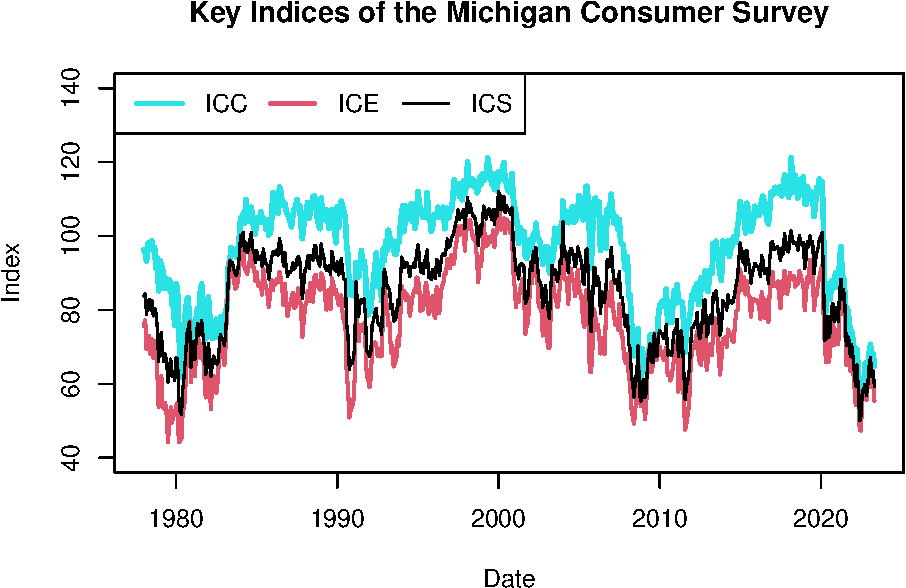
\includegraphics{_main_files/figure-latex/icc-ice-ics-plot-1.pdf}
\caption{\label{fig:icc-ice-ics-plot}Key Indices of the Michigan Consumer Survey}
\end{figure}

The resulting plot, shown in Figure \ref{fig:icc-ice-ics-plot}, displays the historical evolution of the three Michigan consumer survey indices: ICC, ICE, and ICS. These indices are considered leading indicators because they provide early signals about changes in consumer sentiment and economic conditions. They often reflect consumers' expectations and attitudes before these changes are fully manifested in traditional economic indicators, such as unemployment rates or GDP growth.

Consumer sentiment plays a crucial role in shaping consumer behavior, including spending patterns, saving habits, and investment decisions. When consumer confidence is high, individuals are more likely to spend and invest, stimulating economic growth. Conversely, low consumer confidence can lead to reduced spending and investment, potentially dampening economic activity. Hence, these indices can serve as an early warning system for potential shifts in economic activity.

By incorporating the consumer survey indices alongside traditional economic indicators, policymakers and analysts can gain a more comprehensive understanding of the economic landscape. While traditional indicators like unemployment rates provide objective measures of economic conditions, the consumer survey indices offer a subjective perspective, reflecting consumers' beliefs, expectations, and intentions. This subjective insight can provide additional context and help anticipate changes in consumer behavior and overall economic activity.

Therefore, by monitoring both traditional economic indicators and the Michigan consumer survey indices, policymakers and analysts can obtain a more holistic view of the economy, enabling them to make more informed decisions and implement timely interventions to support economic stability and growth.

\hypertarget{excel-file}{%
\subsection{Excel File}\label{excel-file}}

CSV (Comma Separated Values) is a common file format used to store tabular data. As the name suggests, the values in each row of a CSV file are separated by commas. Here's an example of how data is stored in a CSV file:

\begin{itemize}
\tightlist
\item
  Male,8,100,3
\item
  Female,9,20,3
\end{itemize}

In this section, we'll demonstrate how to import a CSV file using real-world Treasury yield curve rates data.

\hypertarget{import-yield-curve-data-in-csv-format-1}{%
\subsubsection*{Import Yield Curve Data in CSV Format}\label{import-yield-curve-data-in-csv-format-1}}
\addcontentsline{toc}{subsubsection}{Import Yield Curve Data in CSV Format}

To obtain the yield curve data, follow these steps:

\begin{enumerate}
\def\labelenumi{\arabic{enumi}.}
\tightlist
\item
  Visit the U.S. Treasury's data center by clicking \href{https://www.treasury.gov/resource-center/data-chart-center}{here}.
\item
  Click on ``Data'' in the menu bar, then select ``Daily Treasury Par Yield Curve Rates.''
\item
  On the data page, select ``Download CSV'' to obtain the yield curve data for the current year.
\item
  To access all the yield curve data since 1990, choose ``All'' under the ``Select Time Period'' option, and click ``Apply.'' Please note that when selecting all periods, the ``Download CSV'' button may not be available.
\item
  To manually save the data as a CSV file, you can copy the data by selecting it and using the Ctrl+C (or Cmd+C) command. Open an Excel file, and use the Ctrl+V (or Cmd+V) command to paste the data into the Excel file.
\item
  Save the Excel file as a CSV file named `yieldcurve.csv' in a location of your choice, ensuring that it is saved in a familiar folder for easy access.
\end{enumerate}

Next, install and load the \texttt{readr} package. Run \texttt{install.packages("readr")} in the console and include the package at the top of your R script. You can then use the \texttt{read\_csv()} or \texttt{read\_delim()} function to import the yield curve data:

\begin{Shaded}
\begin{Highlighting}[]
\CommentTok{\# Load the package}
\FunctionTok{library}\NormalTok{(}\StringTok{"readr"}\NormalTok{)}

\CommentTok{\# Import CSV file}
\NormalTok{yc }\OtherTok{\textless{}{-}} \FunctionTok{read\_csv}\NormalTok{(}\AttributeTok{file =} \StringTok{"files/yieldcurve.csv"}\NormalTok{, }\AttributeTok{col\_names =} \ConstantTok{TRUE}\NormalTok{)}
\end{Highlighting}
\end{Shaded}

\begin{verbatim}
## Warning: One or more parsing issues, call `problems()` on your data frame for details,
## e.g.:
##   dat <- vroom(...)
##   problems(dat)
\end{verbatim}

\begin{verbatim}
## Rows: 8382 Columns: 14
## -- Column specification --------------------------------------------------------
## Delimiter: ","
## chr (6): Date, 1 Mo, 2 Mo, 4 Mo, 20 Yr, 30 Yr
## dbl (8): 3 Mo, 6 Mo, 1 Yr, 2 Yr, 3 Yr, 5 Yr, 7 Yr, 10 Yr
## 
## i Use `spec()` to retrieve the full column specification for this data.
## i Specify the column types or set `show_col_types = FALSE` to quiet this message.
\end{verbatim}

\begin{Shaded}
\begin{Highlighting}[]
\CommentTok{\# Import CSV file using the read\_delim() function}
\NormalTok{yc }\OtherTok{\textless{}{-}} \FunctionTok{read\_delim}\NormalTok{(}\AttributeTok{file =} \StringTok{"files/yieldcurve.csv"}\NormalTok{, }\AttributeTok{col\_names =} \ConstantTok{TRUE}\NormalTok{, }\AttributeTok{delim =} \StringTok{","}\NormalTok{)}
\end{Highlighting}
\end{Shaded}

\begin{verbatim}
## Warning: One or more parsing issues, call `problems()` on your data frame for details,
## e.g.:
##   dat <- vroom(...)
##   problems(dat)
\end{verbatim}

\begin{verbatim}
## Rows: 8382 Columns: 14
## -- Column specification --------------------------------------------------------
## Delimiter: ","
## chr (6): Date, 1 Mo, 2 Mo, 4 Mo, 20 Yr, 30 Yr
## dbl (8): 3 Mo, 6 Mo, 1 Yr, 2 Yr, 3 Yr, 5 Yr, 7 Yr, 10 Yr
## 
## i Use `spec()` to retrieve the full column specification for this data.
## i Specify the column types or set `show_col_types = FALSE` to quiet this message.
\end{verbatim}

In the code snippets above, the \texttt{read\_csv()} and \texttt{read\_delim()} functions from the \texttt{readr} package are used to import a CSV file named ``yieldcurve.csv''. The \texttt{col\_names\ =\ TRUE} argument indicates that the first row of the CSV file contains column names. The \texttt{delim\ =\ ","} argument specifies that the columns are separated by commas, which is the standard delimiter for CSV (\emph{Comma} Separated Values) files. Either one of the two functions can be used to read the CSV file and store the data in the variable \texttt{yc} for further analysis.

To import Excel files, we use the \texttt{readxl} package. To import an Excel file, execute \texttt{install.packages("readxl")} in the console, and then load the package at the start of your R script.

\begin{Shaded}
\begin{Highlighting}[]
\CommentTok{\# Load the package}
\FunctionTok{library}\NormalTok{(}\StringTok{"readxl"}\NormalTok{)}

\CommentTok{\# Print names of all worksheets}
\CommentTok{\# Replace \textquotesingle{}path\textquotesingle{} with your Excel file path}
\CommentTok{\# excel\_sheets(path="car.xlsx")}

\CommentTok{\# Import the sheet you want}
\CommentTok{\# Replace \textquotesingle{}path\textquotesingle{} and \textquotesingle{}sheet\textquotesingle{} with your Excel file path and sheet name}
\CommentTok{\# car \textless{}{-} read\_excel(path="car.xlsx",sheet="Statistics\_A",col\_names=TRUE)}

\CommentTok{\# Import all sheets}
\CommentTok{\# Replace \textquotesingle{}path\textquotesingle{} with your Excel file path}
\CommentTok{\# car\_list \textless{}{-} lapply(excel\_sheets(path="car.xlsx"),read\_excel, path="car.xlsx",col\_names=TRUE)}
\end{Highlighting}
\end{Shaded}

\hypertarget{saving-data}{%
\subsection{Saving Data}\label{saving-data}}

Once the data has been imported and possibly manipulated, it can be saved in various formats.

\begin{Shaded}
\begin{Highlighting}[]
\CommentTok{\# Save data in different formats}
\FunctionTok{save}\NormalTok{(yc, }\AttributeTok{file=}\StringTok{"yieldcurve.RData"}\NormalTok{)}
\FunctionTok{write\_csv}\NormalTok{(}\AttributeTok{x=}\NormalTok{yc, }\AttributeTok{path=}\StringTok{"yieldcurve.csv"}\NormalTok{, }\AttributeTok{na=}\StringTok{"NA"}\NormalTok{)}
\end{Highlighting}
\end{Shaded}

\begin{verbatim}
## Warning: The `path` argument of `write_csv()` is deprecated as of readr 1.4.0.
## i Please use the `file` argument instead.
## This warning is displayed once every 8 hours.
## Call `lifecycle::last_lifecycle_warnings()` to see where this warning was
## generated.
\end{verbatim}

\begin{Shaded}
\begin{Highlighting}[]
\CommentTok{\# Other formats can be used by replacing \textquotesingle{}yieldcurve\textquotesingle{} with your data and \textquotesingle{}path\textquotesingle{} with your desired file name and format}
\end{Highlighting}
\end{Shaded}

For more information on importing data in R, consider taking DataCamp's \href{https://learn.datacamp.com/courses/introduction-to-importing-data-in-r}{Introduction to Importing Data in R} course.

\hypertarget{datacamp}{%
\chapter{DataCamp}\label{datacamp}}

To learn more about R Markdown, consider reading \href{https://bookdown.org/yihui/rmarkdown/}{R Markdown: The Definitive Guide}.

\begin{itemize}
\item
  Create an account on \href{https://www.datacamp.com}{www.datacamp.com} with the free student license you receive by email
\item
  Take \href{https://learn.datacamp.com/courses/introduction-to-r-for-finance}{Introduction to R for Finance} on \href{https://www.datacamp.com}{DataCamp}
\item
  Then take additional courses and explore some of the exciting things you can do with R (and Python)
\item
  For Economics and Business students I recommend

  \begin{itemize}
  \tightlist
  \item
    The entire skill track \href{https://learn.datacamp.com/skill-tracks/finance-fundamentals-in-r}{Finance Fundamentals in R}
  \item
    The entire skill track \href{https://learn.datacamp.com/skill-tracks/applied-finance-in-r}{Applied Finance in R}
  \item
    The entire skill track \href{https://learn.datacamp.com/skill-tracks/importing-cleaning-data-with-r}{Importing \& Cleaning Data with R}
  \item
    The entire skill track \href{https://learn.datacamp.com/skill-tracks/data-visualization-with-r}{Data Visualization with R}
  \item
    The entire skill track \href{https://learn.datacamp.com/skill-tracks/interactive-data-visualization-in-r}{Interactive Data Visualization in R}
  \item
    The entire career track \href{https://learn.datacamp.com/career-tracks/quantitative-analyst-with-r}{Quantitative Analyst with R}
  \item
    \href{https://learn.datacamp.com/courses/reporting-with-rmarkdown}{Reporting with R Markdown} to learn how to write reports
  \item
    \href{https://learn.datacamp.com/skill-tracks/spreadsheet-fundamentals}{Spreadsheet Fundamentals} to learn Excel
  \end{itemize}
\end{itemize}

\hypertarget{assignment}{%
\chapter{Assignment}\label{assignment}}

\begin{enumerate}
\def\labelenumi{\arabic{enumi}.}
\item
  Work through all chapters of Module 1: Introduction to R.
\item
  DataCamp courses:

  \begin{itemize}
  \tightlist
  \item
    A
  \item
    B
  \end{itemize}
\item
  Create
\end{enumerate}

  \bibliography{book.bib,packages.bib}

\end{document}
